\errorcontextlines=9999
\documentclass[
   aspectratio=169, % default is 43
   10pt, % font size, default is 11pt
   % nosectionframes,
   uniqueslidenumber,
   % handout,
   professionalfonts
]{beamer}

\usepackage[T1]{fontenc}
\usepackage[utf8]{inputenc}
\usepackage[sfdefault]{FiraSans}

\usepackage{stmaryrd}
\usepackage[vvarbb]{notomath}
\usepackage{FiraMono}
\usepackage{tikz,forest}
\usepackage{fontawesome}
\usepackage{csquotes}
\usepackage{relsize}
\usepackage{simplebnf}
\usepackage{tabularx,array,makecell,booktabs}
\usepackage{../abstract-interpretation-ltx/absint}
\makeatletter
\def\absint@reflab#1#2{#2}% we do not need labels here
\usetikzlibrary{arrows.meta,decorations.pathmorphing,fit,decorations.pathreplacing,backgrounds,matrix,shadows}
\pgfdeclarelayer{foreground}
\usepackage[glows]{tikzpingus}
\pgfsetlayers{very-background,background,main,middle,foreground}
\def\sbseries{\fontseries{sb}\selectfont}
\def\textsb#1{{\sbseries#1}}
\usepackage[normalem]{ulem}
\usepackage[outline]{contour}
\makeatletter

\DeclareRobustCommand*\xfancyul[2][white]{%
   \def\fancyul@background{#1}%
   \def\ULdepth{1pt}%
   \def\ULthickness{.1ex}%
   \contourlength{.35pt}%
   \mbox{{\color{lightgray}\uline{\phantom{#2}}}\llap{\contour\fancyul@background{#2}}}%
}
\def\link#1#2{\href{#1}{\xfancyul{#2}}}
\tikzset{bottom note/.style={font=\tiny,color=gray}}
\usepackage{../slide-template-uulm/fancybeamer} % use the fancy beamer package
\usepackage{../slide-template-uulm/fancyuulm}
\setpaths{{../slide-template-uulm/}{../slide-template-uulm/logos/}{../slide-template-uulm/empty-slides/}{../xlistings/}}

\usepackage{../code-animation/code-animation}
\def\ca@Strut{\vphantom{\ttfamily\strut}}
\newcounter{NumberOfToolRows}
\providecommand\NumberOfToolRows{0}
\AtEndDocument{
   \immediate\write\@auxout{\string\gdef\string\NumberOfToolRows{\the\value{NumberOfToolRows}}}
}
\def\LeftArrow{\text{\BeginAccSupp{method=escape,ActualText={<-}}\(\leftarrow\)\EndAccSupp{}}}
\def\RightArrow{\text{\BeginAccSupp{method=escape,ActualText={<-}}\(\rightarrow\)\EndAccSupp{}}}
\def\DoubleLeftArrow{\text{\BeginAccSupp{method=escape,ActualText={<<-}}\(\twoheadleftarrow\)\EndAccSupp{}}}
\def\DoubleRightArrow{\text{\BeginAccSupp{method=escape,ActualText={<<-}}\(\twoheadrightarrow\)\EndAccSupp{}}}

\usepackage[fakeminted,print]{../xlistings/xlistings}
\usepackage{multirow}
\xlstsetmintedstyle{plain}
\LoadLanguages{R,Java}
\lstcolorlet{keywordA}{black!70!red}%
\lstcolorlet{keywordB}{black!70!red}%
\lstcolorlet{keywordC}{black!70!red}%
\lstcolorlet{numbers}{black!70!yellow}%
\lstcolorlet{literals}{black!70!purple}%
\def\absintstyle#1{#1}
\urlstyle{same}
\def\AbstractInfo#1{\ensuremath{\mathcolor{gray}{\Lbag}\,#1\,\mathcolor{gray}{\Rbag}}}
\def\Set#1{\ensuremath{\{#1\kern1pt\}}}
\def\IntCC#1#2{\ensuremath{[#1\,..\,#2]}}
\def\IntOC#1#2{\ensuremath{(#1\,..\,#2]}}
\def\IntCO#1#2{\ensuremath{[#1\,..\,#2)}}
\def\IntOO#1#2{\ensuremath{(#1\,..\,#2)}}
\def\S#1{\savebox\TestBox{\footnotesize\absexpr{\Set{#1}}}\ifdim\ht\TestBox>5mm\makebox[5mm][c]{\usebox\TestBox}\else\usebox\TestBox\fi}%
\def\I#1#2{\footnotesize\absexpr{\IntCC{#1}{#2}}}

\colorlet{@}{black}
\usepackage{forest}
\let\RectAtBegin\strut
\tikzset{
   Soft/.style={line join=round,line cap=round},
   All Soft/.style={every path/.append style={Soft}},
   Blob/.style={
      draw=@,
      circle,
      outer sep=2pt,
      minimum size=1.8em
   },
   Blobs/.style={
      every node/.append style={Blob}
   },
   Use/.style={Blob},
   RectRounding/.style={rounded corners=3pt},
   RawRect/.style={
      draw=@,
      rectangle,
      RectRounding,
      % outer sep=2pt,
      minimum size=1.8em,
      inner sep=5pt,
      fill=white,
      execute at begin node={\RectAtBegin},
   },
   RectShadow/.style={
      drop shadow={fill=lightgray!42},
   },
   Rect/.style={
      RawRect,
      RectShadow
   },
   Def/.style={Rect},
   Rects/.style={
      every node/.append style={Rect,minimum width=#1}
   },
   Rects/.default={1.5em},
   Link/.style={
      draw,
      RectRounding,
      Soft,
      -Kite
   },
   Links/.style={
      every path/.append style={Link}
   },
   % for dataflow graphs
   comm/.style={rectangle,draw=gray,text width=9mm,align=center,minimum height=5mm,font=\ttfamily,fill=white,fill opacity=1,drop shadow={fill=lightgray!42}},
   d/.style={comm,rounded corners=2pt}, % variable def
   u/.style={comm,rounded corners=2.5mm}, % variable use % rounded rectangle breaks anchors
   e/.style={comm,rounded corners=2.5mm,densely dotted,thick,fill=white}, % exit point
   F/.style={comm,draw=gray,rounded corners=2pt,fill=white,inner xsep=.5em},
   fc/.style={comm,double,rounded corners=2pt},
   w-back/.style={fill=white,inner sep=1pt},
   T/.style={font=\footnotesize\ttfamily,text=gray},
   code/.style={font=\ttfamily},
   dfidn/.style={
      circle,darkgray,fill opacity=.925,xshift=-1mm,yshift=.15mm,fill=white,draw,minimum size=1.8em,scale=.8,inner sep=-1pt
   },
   olabel/.style={midway,fill=white,rounded corners=2pt,inner sep=2pt,font=\scriptsize\sffamily},
   pos at/.style={above #1=-.5mm,yshift=-.4\baselineskip},
	Line-Of-Text/.style={
      fill=#1,
      draw=none,
      rounded corners=1.5pt,
      inner sep=1pt,
      minimum width=1cm,
      minimum height=6.5pt
   },
   % code sub-styles
   A/.style={Line-Of-Text=SoftTextGray!93!black},
   B/.style={},
   C/.style={Line-Of-Text=SoftGray!93!black},
	ActiveBlob/.style={
      Blob,
      draw=BaseGray, fill=BaseGray
   }
}
\definecolor{BaseGray}{RGB}{66,66,66} % rgb(66,66,66)

\colorlet{SoftGray}{BaseGray!60}
\colorlet{BackGray}{BaseGray!2}
\colorlet{SoftTextGray}{BackGray!60!SoftGray}

\forestset{T/.style={for tree={font=\ttfamily,align=center,l sep=0pt,l sep-=5mm,child anchor=north}}}
\newsavebox\ArchitectureBox
\setbox\ArchitectureBox=\hbox{\tikz[baseline={([yshift=-2mm]current bounding box.center)},scale=1.35]{\draw[rounded corners=.5mm,fill=white,opacity=.8]
(0,0) -| ++(-6mm,8mm) -- ++(4mm,0) |- ++(2mm,-2mm) coordinate (@) -- cycle
([yshift=-1mm]@) -- ++(0,1mm) -- ++(-2mm,2mm) -- ++(-1mm,0);}}
\newsavebox\Parsing
\setbox\Parsing=\hbox{\scalebox{.5}{
\begin{tikzpicture}
   \foreach[count=\i from 0] \Code in {
         {1/C,2/A,3/A},
         {.5/B,1/A,2/A,1/A,1/A},
         {.5/B,2/A,3/A},
         {1/A},
         {},
         {1/A,2/A,6/A},
         {1.5/A,1/A,2/A,.5/B,1/A},
      } {
         \def\XShift{5}
         \foreach \CW/\Style in \Code {
            \ifstrequal{\Style}{B}{\def\RandomSuffix{0}}{\def\RandomSuffix{(rand*0.4mm+0.75mm)}}
            \pgfmathsetmacro\w{3*\CW mm+\RandomSuffix}
            \path[\Style] ([yshift=-2.5mm-1cm,xshift=3.25mm+\XShift pt]0,-\i*0.28*10mm+1mm) rectangle ++(\w pt,-1.75mm);

            \pgfmathsetmacro{\XShift}{\XShift+\w pt+1mm}
            \xdef\XShift{\XShift}
         }
      }
\end{tikzpicture}}}

\errorcontextlines9999

\newsavebox\FirstAst
\setbox\FirstAst=\hbox{\resizebox*!{1.25cm}{\begin{forest}
   for tree={Blob,edge={Soft,-}}
   [[[][,phantom]][[[][,phantom]][]]]
\end{forest}}}
\newsavebox\DataFlow
\setbox\DataFlow=\hbox{\resizebox*!{1.25cm}{\color{lightgray!80!BaseGray}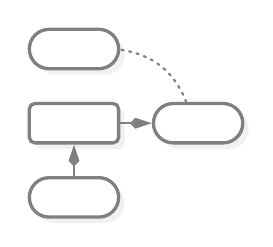
\begin{tikzpicture}[Link/.style={draw,line cap=round,gray,thick},comm/.append style={very thick}]
   \node[d] (0) at (0,0) {};
   \node[u,right=4mm] (1) at (0.east) {};
   \node[u,above=4mm] (2) at (0.north) {};
   \node[u,below=4mm] (3) at (0.south) {};
   \draw[Link,-Kite] (3) -- (0);
   \draw[Link,-Kite] (0) -- (1);
   \draw[Link,dotted] (1) to[bend right] (2);
\end{tikzpicture}}}
\newsavebox\Slicing
\setbox\Slicing=\hbox{\resizebox*!{1.25cm}{\color{lightgray!80!BaseGray}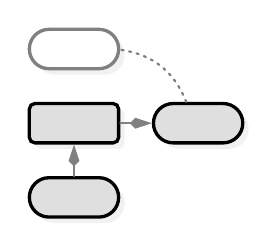
\begin{tikzpicture}[Link/.style={draw,line cap=round,gray,thick},m/.style={draw=black,very thick,fill=lightgray!50!white},comm/.append style={very thick}]
   \node[d,m] (0) at (0,0) {};
   \node[u,m,right=4mm] (1) at (0.east) {};
   \node[u,above=4mm] (2) at (0.north) {};
   \node[u,m,below=4mm] (3) at (0.south) {};
   \draw[Link,-Kite] (3) -- (0);
   \draw[Link,-Kite] (0) -- (1);
   \draw[Link,dotted] (1) to[bend right] (2);
\end{tikzpicture}}}
\newsavebox\Reconstruct
\setbox\Reconstruct=\hbox{\scalebox{.5}{
\begin{tikzpicture}
   \foreach[count=\i from 0] \Code in {
         {1/C,2/A,3/A},
         {.5/B,2/A,3/A},
         {1/A},
         {},
         {1/A,2/A,4/A},
      } {
         \def\XShift{5}
         \foreach \CW/\Style in \Code {
            \ifstrequal{\Style}{B}{\def\RandomSuffix{0}}{\def\RandomSuffix{(rand*0.4mm+0.75mm)}}
            \pgfmathsetmacro\w{3*\CW mm+\RandomSuffix}
            \path[\Style] ([yshift=-2.5mm-1cm,xshift=3.25mm+\XShift pt]0,-\i*0.28*10mm+1mm) rectangle ++(\w pt,-1.75mm);

            \pgfmathsetmacro{\XShift}{\XShift+\w pt+1mm}
            \xdef\XShift{\XShift}
         }
      }
\end{tikzpicture}}}

\tikzset{br/.style={fill=white,draw=black,drop shadow={fill=lightgray!42},minimum width=2.5cm,minimum height=1.5cm,signal,signal from=west,signal to=east,signal pointer angle=125,rounded corners=2pt}}

\newif\ifoverviewParse \overviewParsetrue
\newif\ifoverviewNormalize \overviewNormalizetrue
\newif\ifoverviewDataflow \overviewDataflowtrue
\newif\ifoverviewSlice \overviewSlicetrue
\newif\ifoverviewReconstruct \overviewReconstructtrue

\newsavebox\Overview
\def\StoreOverview#1{%
\setbox\Overview=\hbox{\begin{tikzpicture}[All Soft,k/.style={below,font=\footnotesize,xshift=-.33mm,color=darkgray},m/.style={above,font=\scriptsize,xshift=-.33mm,color=gray},BaseGray,Link/.style={
   draw=SoftGray,
   line width=1.5pt,
   line cap=round,
   line join=round,
   -%
},base/.style={opacity=.35},a/.style={base},b/.style={base},c/.style={base},d/.style={base},e/.style={base},f/.style={base},#1]
   \ifoverviewParse
   \scope[transparency group,b]
   \node[br,right=3mm] (@) at (@.east) {};
   \node (r-conv) at (@) {\usebox\Parsing};
   \node[k] at (@.south) {Parse};
   \endscope
   \fi

   \ifoverviewNormalize
   \scope[transparency group,c]
   \node[br,right=3mm] (@) at (@.east) {};
   \node (first-ast) at (@) {\usebox\FirstAst};
   \node[k] at (@.south) {Normalize};
   \endscope
   \fi
   \ifoverviewDataflow
   \scope[transparency group,d]
   \node[br,right=3mm] (@) at (@.east) {};
   \node (dataflow) at (@) {\usebox\DataFlow};
   \node[k] at (@.south) {Dataflow};
   \endscope
   \fi
   \ifoverviewSlice
   \scope[transparency group,e]
   \node[br,right=3mm] (@) at (@.east) {};
   \node (slicing) at (@) {\usebox\Slicing};
   \node[k] at (@.south) {Slice};
   \endscope
   \fi
   \ifoverviewReconstruct
   \scope[transparency group,f]
   \node[br,right=3mm] (@) at (@.east) {};
   \node (reconstruct) at (@) {\usebox\Reconstruct};
   \node[k] at (@.south) {Reconstruct};
   \endscope
   \fi
\end{tikzpicture}}}

\def\ShowOverview{\node[below left=3.25mm,scale=.6] at(current page.north east) {\usebox\Overview};}

\setcounter{tocdepth}{1}

% bib
\usepackage[style=alphabetic,backend=biber]{biblatex}
\addbibresource{./references.bib}
\addbibresource{./analyzers.bib}

\title{Static Analysis in the Real World}
\subtitle[SQA]{Software Quality Assurance - Static Code Analysis, III}
\author[F. Sihler]{Florian Sihler}
\date{\today} % use a particular date here if needed

\fancylogos{sp,uulm} % define logos that are spread evenly across the bottom of the title slide

\usepackage{../beamer-latex-pdfpc-notes}

\begin{document}

\maketitle[titleimage/title][40]

\mode
<handout>

\begin{frame}{\strut Outline}
% \begin{multicols}{2}
\tableofcontents[hideallsubsections]
% \end{multicols}
\end{frame}

\mode
<all>

\section{Introduction}

\newsavebox\abstractionbox
\begin{lrbox}{\abstractionbox}
\begin{tikzpicture}[line cap=round]
   \pgfonlayer{foreground}
   \draw[Kite-Kite,very thick] (0,3.5) node[below right,yshift=1mm] {\(x(t)\)} |- (8,0) node[above left] {\(t\)}; % time vs. x at tat time
   \endpgfonlayer
   \colorlet{@}{gray}
   \draw[very thick,@] (0,1) plot [smooth] coordinates {(0,1) (1,2) (2,1) (3,2) (4,1) (5,2) (6,1) (7,2) (8,1)}; % x(t)
   \draw[very thick,@] (0,0) plot [smooth] coordinates {(0,0) (1,1) (2,2) (3,2) (4,2.5) (5,2.5) (6,.5) (7,.6) (8,.6)}; % x(t)
   \draw[very thick,@] (0,1.5) plot [smooth] coordinates {(0,1.5) (1,2) (2,2.5) (3,2) (4,2) (5,2.5) (6,2.5) (7,2) (8,2.5)}; % x(t)
      \foreach \i in {0,...,5} {
         \pgfmathsetmacro{\randA}{rnd*0.33}
         \pgfmathsetmacro{\randB}{rand*0.5}
         \pgfmathsetmacro{\randC}{rand*0.4}
         \draw[gray] (0,1.5+\randA) plot [smooth] coordinates {(0,1.5+\randA) (1,2-\randB) (2,2.5-\randA) (3,2-\randB) (4,2+\randA) (5,2.5) (6,2.5+\randA) (7,2-\randA) (8,2.5+\randB)} node[inner sep=0pt] (a-\i) {};
         \draw[gray] (0,0+\randA) plot [smooth] coordinates {(0,0+\randA) (1,1-\randB) (2,2-\randB) (3,2+\randC) (4,2.5-\randA) (5,2.5-\randB) (6,.5+\randC) (7,.6+\randB) (8,.6+\randC)} node[inner sep=0pt] (b-\i) {};
         \draw[gray] (0,1+\randB) plot [smooth] coordinates {(0,1-\randC) (1,2-\randB) (2,1+\randB) (3,2-\randA) (4,1+\randA) (5,2-\randB) (6,1) (7,2-\randC) (8,1+\randA)} node[inner sep=0pt] (c-\i) {};
      }
   % fit to all nodes to get the bounding box
   \node[fit=(a-0) (a-1) (a-2) (a-3) (a-4) (a-5) (b-0) (b-1) (b-2) (b-3) (b-4) (b-5) (c-0) (c-1) (c-2) (c-3) (c-4) (c-5),inner sep=0pt] (big-ghost) {~};
      % \draw[decorate,thick,decoration={brace,amplitude=5pt,raise=2pt},gray] (big-ghost.north east) -- (big-ghost.south east);
   \pgfonlayer{background}
   \pgfinterruptboundingbox
   \fill[red,opacity=.175,even odd rule] plot [smooth] coordinates {(0,0) (1,0.4) (2,0.5) (3,1) (4,.8) (5,1) (6,.1) (7,0.2) (8.03,.2) (8.03,3) (7,2.8) (6,3) (5,2.95) (4,2.85) (3,2.75) (2,2.65) (1,2.5) (0,2) } -- cycle (6,1.85) circle[radius=4mm]; 
   \endpgfinterruptboundingbox
      \node (@b1) at (6,1.85) {\small\faBug};
      \node (@b2) at (3,.35) {\small\faBug};
      \node (@b3) at (7,2.5) {\small\faBug};
      \node[above left=-1mm,green] at(@b2.south east) {\scriptsize\faCheck};
      \node[above left=-1mm,green] at(@b1.south east) {\scriptsize\faCheck};
      \node[above left=-1mm,yshift=1pt,orange] at(@b3.south east) {\scriptsize\faQuestion};
   \endpgfonlayer
   \path[use as bounding box] (0,0) rectangle (8,3.5);
\end{tikzpicture}
\end{lrbox}

\begin{frame}{What we have\ldots}
\frametitle<-8>{\strut What we have\ldots}%
\frametitle<9->{\strut\textcolor{gray}{What we have\ldots~}Theory}%
\pgfmathsetseed{42}%
\begin{uncoverenv}<2->  
\begin{tikzpicture}[baseline={([yshift=-.5ex]current bounding box.center)},line cap=round]
   \tikzset{@/.style={opacity=1}}
   \def\scaler{1}
   \only<4->{\def\scaler{0.5}\tikzset{@/.style={opacity=.5,scale=.5,every node/.style={transform shape}}}}
   \scope[transparency group, @]
   \node (@) at (0,0) {\usebox\abstractionbox};
   \onslide<3>{
   \draw[decorate,thick,decoration={brace,amplitude=8pt*\scaler,raise=2pt},line width=0.5pt*\scaler] (@.north east) to[edge node={node [right=3.5mm] {Abstractions}}] (@.south east);
   }
   \onslide<4->{%
      \node[below] at(@.south) {Abstractions};
   }
   \endscope
\end{tikzpicture}
\begin{uncoverenv}<5->
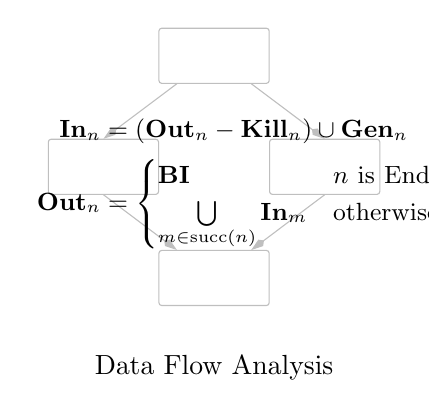
\begin{tikzpicture}[r/.style={rectangle,draw,minimum width=2cm,minimum height=1cm,rounded corners=1pt},baseline={([yshift=-.5ex]current bounding box.center)},line cap=round]
   \tikzset{@/.style={opacity=1}}
   \def\scaler{1}
   \only<7->{\def\scaler{0.5}\tikzset{@/.style={opacity=.5,scale=.5,every node/.style={transform shape}}}}
   \scope[@]
   \scope[black!25!white,scale=.7,every node/.style={transform shape}]
   \node[r] (@) at(0,0) {};
   \node[r, below left=1cm] (@a) at(@.south) {};
   \node[r, below right=1cm] (@b) at(@.south) {};
   \node[r,below=1cm] (@c) at(current bounding box.south) {};
   \draw[-Kite] (@) -- (@a.north);
   \draw[-Kite] (@) -- (@b.north);
   \draw[-Kite] (@a.south) -- (@c);
   \draw[-Kite] (@b.south) -- (@c);
   \endscope
   \node[align=center,text width=4.5cm] at(current bounding box.center) {\small%
\begin{align*}
   \mathbf{In}_n &= (\mathbf{Out}_n - \mathbf{Kill}_n) \cup \mathbf{Gen}_n \\
   \mathbf{Out}_n &= \begin{cases}
      \mathbf{BI} & n \text{~is End} \\
      \bigcup\limits_{m \in \text{succ}(n)} \mathbf{In}_m & \text{otherwise}
   \end{cases}
\end{align*}
   };
   \onslide<6->{
      \node[below=5mm] at(current bounding box.south) {Data Flow Analysis};
   }
   \endscope
\end{tikzpicture}
\end{uncoverenv}
\hspace*{4.5em}\onslide<8->{\large\ldots}
\end{uncoverenv}
\end{frame}

\newsavebox\CodeFile
\begin{lrbox}{\CodeFile}
\scalebox{1.45}{%

\begin{tikzpicture}
   \draw[rounded corners=1.5pt,fill=white] (0,0) |- ++(.6,-.8) [sharp corners] -- ++(0,.6) -- ++(-.2,.2) coordinate (@rl) [rounded corners=2pt] -- cycle (@rl) |- ++(.2,-.2);
   \draw[thick,line cap=round,lightgray] (.1,-.1) -- ++(.2,0)
      % for what have I written random code generation? :C 
      (.1,-.15) -- ++(.1,0) ++(.05,0) -- ++(.1,0)
      (.125,-.2) -- ++(.15,0)++(.05,0)--++(.025,0)
      (.1,-.25) -- ++(.3,0)
      (.125,-.3) --++(.2,0)++(.05,0)--++(.05,0)
      (.125,-.35) --++(.15,0)++(.05,0)--++(.1,0)
      (.15,-.4)--++(.2,0)
      (.15,-.4)--++(.1,0)++(.05,0)--++(.05,0)
      (.125,-.45)--++(.05,0)
      (.1,-.5)--++(.066,0)++(.05,0)--++(.15,0)
      (.1,-.6)--++(.15,0)++(.05,0)--++(.15,0)
      (.1,-.65)--++(.2,0)
      (.1,-.7)--++(.1,0)++(.05,0)--++(.15,0)
   ;
\end{tikzpicture}}
\end{lrbox}
\newsavebox\MagicPenguin
\savebox\MagicPenguin{\tikz{\pingu[witch hat,eyes wink,wings wave,bee,blush,santa beard]}}
\newsavebox\MagicPenguinTwo
\savebox\MagicPenguinTwo{\tikz{\pingu[witch hat,eyes shiny,bee,santa beard]}}
\begin{frame}{What we want\ldots}
   \frametitle<1>{\strut What we want\ldots~}%
   \frametitle<2->{\strut\textcolor{gray}{What we want\ldots~}Tools}%
   \centering\kern1.345em
   \begin{uncoverenv}<3->
   \begin{tikzpicture}[o/.style={outer sep=0pt,inner sep=0pt},line cap=round,Rect/.style={draw,rectangle,rounded corners=3pt,inner sep=4pt,outer sep=1mm},draw=gray,every path/.append style={thick}]
      \node[o] (@) at (0,0) {\usebox\CodeFile};
      \pgfonlayer{background}
      \scope[transparency group,opacity=.4]
      \node[o,rotate around={-30:(@.south east)},anchor=south east] at(@.south east) {\usebox\CodeFile};
      \node[o,rotate around={-12:(@.south east)},anchor=south east] at(@.south east) {\usebox\CodeFile};
      \endscope
      \endpgfonlayer
      \node[below] at(@.south) {\small Project};
      \onslide<3->{
         \node[right=1.33cm,Rect,minimum width=4.5em] (@magic) at(@.east) {~\vphantom{Magic}{\only<8->{\only<9->{\color{gray!34}}\clap{Magic}}}\only<9->{\clap{\kern-.8pt\textbf{Tools}}}~\null};
         \draw[-Kite] ([xshift=5mm]@.east) -- (@magic.west);
      }
      % and how can we achieve that?... magic :sparkles: but as there is no magic, we need tools... and algorithms
      \onslide<8->{
         \node[above right,xshift=1.3mm] at(@magic.north west) {\scalebox{.45}{\only<-8|handout:0>{\kern-8.5pt\usebox\MagicPenguin}\only<9->{\usebox\MagicPenguinTwo}}};
      }
      \coordinate (@) at(@magic.east);
      \foreach[count=\i] \usecase/\targeti in {Security/4, Maintenance/5, Comprehension/6, Optimization/7, Usability/7, \ldots/7} {
      \pgfmathsetmacro\rot{-11*\i+38.75}
         \onslide<\targeti->{
            \node[right=1cm,Rect,rotate around={\rot:([xshift=-9mm]@.east)},minimum width=8em,fill=white] (@uc-\i) at (@.east) {\strut\usecase};
            \draw[-Kite,sharp corners] (@.east) -- ++(4.2mm,0) [rounded corners=1pt] arc (0:\rot:9mm) -- (@uc-\i.west);
         }
      }
      \onslide<11->{
         \scope[gray]
         \node[right] at (@uc-1.east) {\small injections, leaks,~\ldots};
         \node[right] at (@uc-2.east) {\small code clones, deprecation,~\ldots};
         \node[right] at (@uc-3.east) {\small documentation, structure,~\ldots};
         \node[right] at (@uc-4.east) {\small better algorithms, memoization,~\ldots};
         \node[right] at (@uc-5.east) {\small color deficiency, size,~\ldots};
         \node[right] at (@uc-6.east) {\small \only<-11|handout:0>{\ldots}\only<12->{architecture recovery, refactoring,~\ldots}};
         \endscope
      }
      \onslide<13->{
         \draw[Kite-] (@magic.south) -- ++(0,-.66) node[below,align=center,font=\footnotesize] {SonarQube\rlap{\textsuperscript{1}}, Teamscale\rlap{\textsuperscript{2}},\\lintr\rlap{\textsuperscript{3}}, CodeQL\rlap{\textsuperscript{4}}, \ldots};
      }
   \end{tikzpicture}

   \begin{tikzpicture}[overlay,remember picture]
      \onslide<10->{%
         \node[above=9mm,lightgray] at(current page.south) {\footnotesize\enquote{Any sufficiently advanced technology is indistinguishable from magic.} --- Arthur C. Clarke};% 3rd law
      }
      \only<13->{\node[bottom note,above right,yshift=5mm] at(current page.south west) {%
         \textsuperscript{1}\,\href{https://www.sonarsource.com/}{sonarsource.com}, \textsuperscript{2}\,\href{https://teamscale.com/}{teamscale.com}, \textsuperscript{3}\,\href{https://lintr.r-lib.org/}{lintr.r-lib.org}, \textsuperscript{4}\,\href{https://codeql.github.com/}{codeql.github.com}%
      };}
   \end{tikzpicture}
   % TODO: tool examples
   % rather list concrete problems than tools
\end{uncoverenv}
\end{frame}

\usetikzlibrary{backgrounds,graphs,arrows.meta,decorations.pathreplacing}

\definecolor{BaseGray}{RGB}{66,66,66} % rgb(66,66,66)

\colorlet{SoftGray}{BaseGray!40}
\colorlet{BackGray}{BaseGray!5}
\colorlet{SoftTextGray}{BackGray!60!SoftGray}


\tikzset{
   FunctionDef/.style={
      draw=BaseGray,
      fill=BaseGray,
      minimum width=1.55cm,
      minimum height=1cm,
      text=white,
      font=\bfseries,
      text centered,
      inner sep=0pt,
      rounded corners=1mm,
      outer sep=2pt
   },
   Blob/.style={
      draw=SoftGray,
      fill=SoftGray,
      minimum size=4mm,
      text=white,
      circle,
      font=\bfseries,
      text centered,
      inner sep=0pt,
      outer sep=2pt
   },
   Def/.style={
      Blob,
      rectangle, rounded corners=1mm
   },
   ActiveBlob/.style={
      Blob,
      draw=BaseGray!80!white, fill=BaseGray!80!white
   },
   FunctionBack/.style={
      fill=BackGray,
      % draw=SoftGray,
      rounded corners=2mm,
      rectangle
   },
   Link/.style={
      draw=SoftGray,
      line width=1.5pt,
      line cap=round,
      line join=round,
      -%
   },
   FuncLink/.style={
      Link,
      draw=SoftGray,
      dotted
   },
   Cursor/.style={
      fill=BackGray,
      draw=BaseGray,
      line join=round,
      line cap=round
   },
   Hover-Over/.style={
      fill=BackGray,
      draw=SoftGray,
      opacity=.5,
      draw opacity=1,
      rounded corners=1mm,
      line join=round,
      line cap=round
   },
   Line-Of-Text/.style={
      fill=#1,
      draw=none,
      rounded corners=1.5pt,
      inner sep=1pt,
      minimum width=1cm,
      minimum height=6.5pt
   },
   Input-Base/.style={
      fill=BackGray,
      draw=SoftGray,
      rounded corners=1mm,
      inner sep=1pt,
      minimum width=2cm,
      minimum height=12pt
   },
   % code sub-styles
   A/.style={Line-Of-Text=SoftTextGray},
   B/.style={},
   C/.style={Line-Of-Text=SoftGray},
   path image shift/.style={},
   path image/.style 2 args={path picture={\node at ([path image shift]path picture bounding box.center) {\includegraphics[width=#2]{#1}};}},
}


\newcommand\Back[4][]{
   \pgfonlayer{background}
   \fill[FunctionBack,#1] ([xshift=-2mm,yshift=-2mm]#2.south west) rectangle ([xshift=2mm,yshift=2mm]#3.north east);
   \coordinate (#4@north) at([yshift=2mm]0,0|-#3.north);
   \coordinate (#4@west) at([xshift=-2.5mm]0,0-|#2.west);
\endpgfonlayer
}
\newsavebox\UiBox
\begin{lrbox}{\UiBox}
\begin{tikzpicture}
   \node[FunctionDef] (F) at (0,0) {};

   \scope[shift={(F.south)},yshift=-1.5cm]
      \node[Def] (a1) at (-1,0) {};
      \node[Blob] (b1) at (.5,-.25) {};
      \node[ActiveBlob] (c1) at (1.55,-1.35) {};
      \node[Blob] (d1) at (-0.5,-1.6) {};
      \node[Blob] (e1) at (1.8,.25) {};
      \node[Blob] (f1) at (-2.2,-1.5) {};

      \graph[edges={Link}] {
         (a1) -> { (b1), (c1) } -> (d1) -> (e1) -> (a1),
         (f1) -> { (a1), (d1) }
      };

      \Back{f1}{e1}{f1}

      \draw[FuncLink] (f1@north) -- (F.south);
   \endscope

   \node[Blob] (a) at (2.5,0) {};
   \node[Blob] (b) at (1.5,1) {};
   \node[Blob] (c) at (3,2) {};
   \node[Blob] (d) at (-2.5,0.5) {};
   \node[Def] (e) at (-2.5,1.5) {};
   \node[Blob] (f) at (-3,2.5) {};
   \node[Blob] (g) at (-3.5,-1) {};
   \node[Blob] (h) at (-3,-2.5) {};

   \node[FunctionDef] (F2) at(5,-.5) {};
   \node[Blob] (u) at(5.5,1) {};

   \scope[shift={(F2.east)},xshift=1.5cm]

      \node[Blob] (a2) at (0,1.15) {};
      \node[Def] (b2) at (.75,1.85) {};
      \node[Blob] (c2) at (-.5,-.85) {};

      \node[Blob] (d2) at (1.33,0.25) {};
      \node[FunctionDef] (e2) at (2,-.75) {};

      \node[Blob] (f2) at (3.75,1.5) {};
      \node[Blob] (g2) at (2.75,2.5) {};

      \scope[shift=(e2.south), yshift=-1cm]
         \node[ActiveBlob] (a3) at (-1,0) {};
         \node[Blob] (b3) at (1,0) {};
         \draw[Link] (a3) -- (b3);
         \Back[white]{a3}{b3}{a3} % for coordinate
      \endscope

      \coordinate (ll) at ([yshift=-2mm]a3.south west-|c2.west);
      \coordinate (ur) at (f2.north east|-g2.north);

      \Back{ll}{ur}{e2}
      \draw[FuncLink] (e2@west) -- (F2.east);

      % draw inner later
      \Back[white]{a3}{b3}{xx} % for the overlay :D
      \draw[FuncLink] (a3@north) -- (e2.south);

      \graph[edges={Link}] {
         (a2) -> (b2) -> { (c2) , (d2) },
         (d2) -> { (e2), (f2) },
         (f2) -> (g2),
         (c2) -> (a3)
      };
   \endscope

   \graph[edges={Link}] {
      (F) -> { (a), (b) },
      (a) -> (e1),
      (b) -> (c) -> (b2),
      (b) -> (d) -> { (F), (e) },
      (e) -> (f) -> (c),
      (d) -> (g) -> (h) -> (f1),
      (u) -> (F2)
   };

   \coordinate (cursor-pos) at ([xshift=-1.65mm,yshift=2mm]F2.south east);
   \draw[Cursor,rotate around={28:(cursor-pos)}]  [rounded corners=2.25pt] (cursor-pos)  [rounded corners=2.25pt] -- ++(4pt,-9.5pt) [rounded corners=2pt] -- ++(-4pt,3pt) [rounded corners=2.25pt]-- ++(-4pt,-3pt) -- cycle;
   \node[below left,xshift=-1mm,yshift=1.15mm,Hover-Over,minimum width=1.25cm,minimum height=6mm] (hoverover) at(cursor-pos) {%
      %
   };
   % \scope[opacity=.95,transparency group]
      \fill[Line-Of-Text=SoftGray] ([shift={(2pt,-2pt)}]hoverover.north west) rectangle ++(7.5mm,-4pt);
      \fill[Line-Of-Text=SoftTextGray] ([shift={(2pt,-7.5pt)}]hoverover.north west) rectangle ++(11mm,-3pt);
      \fill[Line-Of-Text=SoftTextGray] ([shift={(2pt,-7.5pt-4.5pt)}]hoverover.north west) rectangle ++(8mm,-3pt);
   % \endscope

   % TODO: outsource window?
   \coordinate (wul) at ([shift={(-5mm,6mm)}]current bounding box.north west);
   \coordinate (wur) at ([shift={(5mm,6mm)}]current bounding box.north east);
   \draw[thin,rounded corners=3pt,SoftGray] ([shift={(-5mm,-5mm)}]current bounding box.south west) rectangle (wur);
   % just "overlay" the top :D
   \filldraw[SoftGray] ([yshift=-1mm]wul) coordinate (@) -- (wur|-@) [rounded corners] |- ([yshift=2.5mm]wul) [sharp corners] -- cycle;

   \fill[Line-Of-Text=BackGray] ([yshift=1.35mm,xshift=4pt]wul) rectangle ++(2cm,-1.27mm);
   \node[above left,BackGray] at([yshift=-1.33mm,xshift=-1mm]wur) {\smash{\scalebox{.9}{\scriptsize\faAngleDown~~\faAngleUp~~\faTimesCircle}}};

   \coordinate (root control window) at(current bounding box.south west);

   \scope[shift={(current bounding box.south east)},shift={(-7cm,4.5mm)}]
      \coordinate (wul) at (0,0);
      \coordinate (wur) at (8.5,0);

      \draw[thin,rounded corners=3pt,SoftGray,fill=white] (0,-5) rectangle (wur);

      % code line
      \draw[thin,BackGray] ([xshift=1cm,yshift=-1mm]wul) coordinate (@) -- (@|-0,-5);
      % line numbers and code
      \foreach[count=\i from 0] \Code in {
         {1/A,0.5/A,5/C,2/A},
         {1.5/B,3/A,0.5/A,2/A},
         {},
         {1.5/B,0.5/A,3/A},
         {1/A},
         {},
         {5/A,0.5/A,2/A},%
         {0.5/A,5/A,3/A,0.5/A,2/A,5.5/A},
         {},
         {1/C,0.5/A,1/A,0.5/A,1/A,0.5/A,0.15/B,0.5/A},
         {1.5/B,3/A,0.5/A,1/C,2/A,1.5/A,1/C,1.5/A},
         {1.5/B,0.75/A,0.5/A,1.5/A,0.5/A,1/A},
         {1.5/B,3/A,0.5/A,2/A},
         {1.5/B,2/A,0.5/A,2/A},
         {1/A}%
      } {
         \ifnum\i<6 \def\Width{4mm} \else \def\Width{6mm} \fi
         \fill[Line-Of-Text=BackGray] ([yshift=-1mm,xshift=8mm]wul|-0,-\i*0.33*10mm+1mm) rectangle ++(-\Width,-2mm);
         \def\XShift{5}
         \foreach \CW/\Style in \Code {
            \ifstrequal{\Style}{B}{\def\RandomSuffix{0}}{\def\RandomSuffix{(rand*0.4mm+0.75mm)}}
            \pgfmathsetmacro\w{3*\CW mm+\RandomSuffix}
            \path[\Style] ([yshift=-1mm,xshift=1cm+\XShift pt]wul|-0,-\i*0.33*10mm+1mm) rectangle ++(\w pt,-2mm);

            \pgfmathsetmacro{\XShift}{\XShift+\w pt+1.5mm}
            \xdef\XShift{\XShift}
         }
      }

      % slider
      \draw[Line-Of-Text=SoftTextGray,rounded corners=.325mm] ([yshift=-4cm+5mm,xshift=-1mm]wur) rectangle ++(-.75mm,-1cm);

      % just redraw the frame :D
      \draw[thin,rounded corners=3pt,SoftGray] (0,-5) rectangle (wur);

      \filldraw[SoftGray] ([yshift=-1mm]wul) coordinate (@) -- (wur|-@) [rounded corners] |- ([yshift=2.5mm]wul) [sharp corners] -- cycle;

      \fill[Line-Of-Text=BackGray] ([yshift=1.35mm,xshift=4pt]wul) rectangle ++(1.66cm,-1.27mm);
      \node[above left,BackGray] at([yshift=-1.33mm,xshift=-1mm]wur) {\smash{\scalebox{.9}{\scriptsize\faAngleDown~~\faAngleUp~~\faTimesCircle}}};

   \endscope

   % window for controls
   \scope[shift={(root control window)},shift={(-1cm,-5mm)}]
      \draw[thin,rounded corners=3pt,SoftGray,fill=white] (0,-4) rectangle ++(8.33cm,4cm);
      \coordinate (wul) at (0,0);
      \coordinate (wur) at (8.33,0);

      \node[Input-Base,minimum width=6cm,below right=3mm] (slice-criterion-input) at (wul) {};
      \fill[Line-Of-Text=SoftTextGray] ([yshift=1mm,xshift=4pt]slice-criterion-input.west) rectangle ++(1.25cm,-2mm);
      \fill[Line-Of-Text=SoftTextGray] ([yshift=1mm,xshift=4pt+1.25cm+2mm]slice-criterion-input.west) rectangle ++(1cm,-2mm);

      % frame stuff
      \filldraw[SoftGray] ([yshift=-1mm]wul) coordinate (@) -- (wur|-@) [rounded corners] |- ([yshift=2.5mm]wul) [sharp corners] -- cycle;
      \node[right=1mm,SoftGray,] at(slice-criterion-input.east) {\tiny\faChevronRight~~~~~\faPieChart~~\faUpload~~\faDownload};

      % logging window
      \draw[rounded corners=3pt,BackGray,fill=white] ([xshift=3mm,yshift=-1cm]wul) rectangle ([xshift=-3mm,yshift=-3.7cm]wur);

      % log
      \foreach[count=\i from 0] \Code in {
         {1/A,2/A,6/A,1/B,3/A},
         {1.5/B,3/A,2/A,2/A,1/A},
         {1.5/B,2/A,3/A,1/A,2/A,3/A,1/A},
         {1.5/B,4/A,1/A},
         {1.5/B,3/A,2/A,2/A,1/A},
         {1.5/B,3/A,1/A,4/A,1/A},
         {},
         {1/A,2/A,6/A},
         {1/A,2/A,3/A,1.5/A,2.5/A},
      } {
         \def\XShift{5}
         \foreach \CW/\Style in \Code {
            \ifstrequal{\Style}{B}{\def\RandomSuffix{0}}{\def\RandomSuffix{(rand*0.4mm+0.75mm)}}
            \pgfmathsetmacro\w{3*\CW mm+\RandomSuffix}
            \path[\Style] ([yshift=-2.5mm-1cm,xshift=3.25mm+\XShift pt]wul|-0,-\i*0.28*10mm+1mm) rectangle ++(\w pt,-1.75mm);

            \pgfmathsetmacro{\XShift}{\XShift+\w pt+1mm}
            \xdef\XShift{\XShift}
         }
      }

      % slider
      \draw[Line-Of-Text=SoftTextGray,rounded corners=.325mm] ([yshift=-2cm+3mm,xshift=-4mm]wur) rectangle ++(-.75mm,-1cm);

      % head
      \fill[Line-Of-Text=BackGray] ([yshift=1.35mm,xshift=4pt]wul) rectangle ++(5mm,-1.27mm);
      \fill[Line-Of-Text=BackGray] ([yshift=1.35mm,xshift=4pt+6.5mm]wul) rectangle ++(1cm,-1.27mm);
      \node[above left,BackGray] at([yshift=-1.33mm,xshift=-1mm]wur) {\smash{\scalebox{.9}{\scriptsize\faAngleDown~~\faAngleUp~~\faTimesCircle}}};
   \endscope
\end{tikzpicture}
\end{lrbox}


\begin{frame}{\strut What do they\ldots~do?}
% they take input, textual, syntactical, semantic (call graphs, pdg, ...), metadata, historical information, requirements, annotations (types, contracts), ...
\hspace*{-3.5mm}
\begin{tikzpicture}[o/.style={outer sep=0pt,inner sep=0pt}]
   \onslide<2->{%
      \node[o] (@) at (0,0) {\usebox\CodeFile};
      \node[above=2.5mm,xshift=1.15mm,gray] at(@.north) {\tiny They take \textbf{\normalsize Input}};
   }
   \pgfonlayer{background}
   \onslide<2->{%
   \scope[transparency group,opacity=.4]
   \node[o,rotate around={-30:(@.south east)},anchor=south east] at(@.south east) {\usebox\CodeFile};
   \node[o,rotate around={-12:(@.south east)},anchor=south east] at(@.south east) {\usebox\CodeFile};
   \endscope}
   \endpgfonlayer
   \begin{uncoverenv}<3->
   \coordinate (@) at(@.east);
   \foreach[count=\i] \usecase/\targeti in {{\raisebox{1pt}{Textual}}/4,Syntactical/5, Semantical/6, Historical/7, Annotated/8, {\only<-9|handout:0>{\ldots}\only<10->{\raisebox{-3pt}{Metadata,~\ldots}}}/9} { % program spectra, hardware, contexts, ...
   \pgfmathsetmacro\rot{-24*\i+66}
      \onslide<\targeti->{
         \path ([xshift=.5mm]@.east)++(\rot+10:1mm) coordinate (@a);
         \fill[opacity=.18,gray] (@a.east) -- ++(\rot:1.5cm) arc (\rot:\rot+20:1.5cm) -- cycle;
         \draw[thick,gray] (@a.east)++(\rot:1.5cm) arc (\rot:\rot+20:1.5cm);
         \path (@a.east) -- ++(1.05*\rot+10:1.6cm) node[right,font=\small,darkgray] (@uc-\i) {\vphantom{a}\smash{\usecase}};
      }
   }
   \node[above=1.65mm,xshift=1mm,gray] at(current bounding box.north) {\tiny And use \textbf{\normalsize Perspectives} \rlap{(often combined)}};
   \end{uncoverenv}
   \onslide<11->{%
      \draw[Kite-,gray] ([xshift=6.25mm,yshift=-1mm]current bounding box.south) to[out=-90,in=0] ++(-4.5mm,-5mm) node[below left,yshift=.42\baselineskip,align=right,text width=2.5cm,font=\tiny] {Some of those are the result of other static or dynamic analyses};
   }
   \begin{uncoverenv}<12->
      \node[right,yshift=-2mm,xshift=1cm,align=left,font=\small,darkgray,text width=3.25cm] (@techn) at(current bounding box.east){{\onslide<13->{\subnode{tc-search}{Text/Code Search}\strut}}~\\[4mm]\strut{\onslide<14->{\subnode{clustering}{Clustering}}}~\\[4mm]\strut{\onslide<15->{\subnode{ai}{Abstract Domains}}}~\\[4mm]\strut{\onslide<16->{\subnode{df-constraints}{Dataflow Constraints}}}~\\[1mm]\strut{\onslide<16->{\centerline{\footnotesize\(\vdots\)}}}};
      \onslide<12->{
         \node[above=2.5mm,gray,xshift=-4.5mm] at(@techn.north) {\tiny To apply \textbf{\normalsize Theory}};
      }
   \end{uncoverenv}
   \scope[gray,line cap=round]
   \only<17->{
      \draw ([yshift=1.5pt]@uc-1.east) -- ([yshift=-2.5mm]@techn.north west);
      \draw ([yshift=1.5pt]@uc-2.east) -- ([yshift=-2.5mm]@techn.north west);
      \draw[densely dotted] ([yshift=1.5pt]@uc-3.east) -- ([yshift=-2.5mm]@techn.north west);
   }
   \only<18->{
      \draw ([yshift=1.5pt]@uc-1.east) -- ([yshift=-10.5mm]@techn.north west);
      \draw ([yshift=0pt]@uc-2.east) -- ([yshift=-10.5mm]@techn.north west);
      \draw ([yshift=1.5pt]@uc-4.east) -- ([yshift=-10.5mm]@techn.north west);
      
      \draw ([yshift=-1pt]@uc-2.east) -- ([yshift=-18.5mm]@techn.north west);
      \draw ([yshift=-1pt]@uc-3.east) -- ([yshift=-18.5mm]@techn.north west);
      \draw ([yshift=1.5pt]@uc-5.east) -- ([yshift=-18.5mm]@techn.north west);
      
      \draw ([yshift=-1pt]@uc-2.east) -- ([yshift=-26mm]@techn.north west);
      \draw ([yshift=-1pt]@uc-3.east) -- ([yshift=-26mm]@techn.north west);
   }
   \endscope
   \begin{uncoverenv}<19->
      
      \onslide<20->{\node[right=7.5mm] (@) at(current bounding box.east) {\resizebox*!{2.85cm}{\usebox\UiBox}};
      \scope[transparency group,opacity=.5,every path/.append style={line cap=round,line width=.5pt}]
         \draw[-Kite,gray] ([yshift=-2.5mm,xshift=-6.5mm]@techn.north east) to[out=0,in=180] ([xshift=1.5mm,yshift=-6.35mm]@.west);
         \draw[-Kite,gray] ([yshift=-10.5mm,xshift=-18.5mm]@techn.north east) to[out=0,in=180] ([xshift=7.15mm,yshift=-1.35mm]@.west);
         \draw[-Kite,gray] ([yshift=-18.5mm,xshift=-6.25mm]@techn.north east) to[out=0,in=180] ([xshift=26.15mm,yshift=-9.35mm]@.west);
         \draw[-Kite,gray] ([yshift=-26mm,xshift=-2.5mm]@techn.north east) to[out=0,in=180] ([xshift=26.15mm,yshift=-9.35mm]@.west);
      \endscope
      }
      \node[above, gray] at(@.north) {\tiny And \textbf{\normalsize Communicate} or \textbf{\normalsize Use} results};
   \end{uncoverenv}
\end{tikzpicture}
\end{frame}


\section{Real-World Static Analyzers}

% #1 url #2 name
\newcommand*\Logo[3][3cm]{\href{#2}{\includegraphics[height=#1,width=
#1,keepaspectratio]{logos/#3.png}}}
\def\mark{\bfseries\large}
\definecolor{infercolor}{RGB}{123, 40, 227}
\def\getsecond#1#2{#2}
\begin{frame}<-16|handout:1,2>[label=tool-slide]{Let's Look at Tools}
\vspace*{-2.95\baselineskip}%
\only<16-|handout:2->{\let\href\getsecond}% avoid behind links on these slides
\begin{tikzpicture}[remember picture]
   \tikzset{@/.style={}}
   \only<2->{\tikzset{@/.style={opacity=0}}}
   \node[@] (sec) at (-2,0) {\bfseries Security};
   \node[@] (mai) at (7,-3) {\bfseries Maintenance};
   \node[@] (com) at (6,2) {\bfseries Comprehension};
   \node[@] (opt) at (9,-1) {\bfseries Optimization};
   \node[@] (sec) at (1.5,-1.75) {\bfseries Usability};
   % TODO: block of compilers; language servers
   \onslide<3->{
      \node[xshift=-2.5mm,yshift=2mm] (sonar) at (current bounding box.center) {\Logo{https://www.sonarsource.com/}{sonar}};
   }
   \onslide<4->{
      \node[xshift=-15mm,yshift=12mm] (teamscale) at (current bounding box.center) {\Logo{https://teamscale.com/}{teamscale}};
   }
   \onslide<5->{
      \node[xshift=20mm,yshift=11mm] (fbinfer) at (current bounding box.center) {\raisebox{-.25\height}{\Logo[8mm]{https://fbinfer.com/}{fb-infer}}~{\color{infercolor}\large\textsb{Infer}}};
      \node[xshift=32mm,yshift=-19mm] (frama-c) at (current bounding box.center) {\Logo{https://frama-c.com/}{frama-c}};
      \node[xshift=-22mm,yshift=-10mm] (eslint) at (current bounding box.center) {\Logo[1.25cm]{https://eslint.org/}{eslint}};
      \node[xshift=56.5mm,yshift=8mm] (lisa) at (current bounding box.center) {\Logo[2cm]{https://github.com/lisa-analyzer/lisa}{lisa}};
      \node[xshift=-42.5mm,yshift=1mm] (codeql) at (current bounding box.center) {\raisebox{-.25\height}{\Logo[6.25mm]{https://github.com/lisa-analyzer/lisa}{codeql}}~\textsb{CodeQL}};
      \node[xshift=0mm,yshift=22mm] (astree) at (current bounding box.center) {\raisebox{-.25\height}{\Logo[26.25mm]{https://www.absint.com/astree/index.htm}{astree}}};
      \node[xshift=7mm,yshift=-16mm] (mopsa) at (current bounding box.center) {\raisebox{-.25\height}{\Logo[16mm]{https://mopsa.lip6.fr/}{mopsa}}};
      \node[xshift=-38.5mm,yshift=20mm] (liquidhs) at (current bounding box.center) {\raisebox{-.25\height}{\Logo[25mm]{https://ucsd-progsys.github.io/liquidhaskell/}{liquidhaskell}}};
      \node[xshift=12.5mm,yshift=38mm] (sootup) at (current bounding box.center) {\Logo[22.5mm]{https://github.com/soot-oss/sootup}{sootup}};
      \node[xshift=40.5mm,yshift=22mm] (flowr) at (current bounding box.center) {\Logo[2.1cm]{https://github.com/flowr-analysis/flowr}{flowR}};
      \node[xshift=55.5mm,yshift=11mm] (lintr) at (current bounding box.center) {\Logo[1.4cm]{https://github.com/r-lib/lintr}{lintr}};
   }
   \onslide<6->{
      \node[xshift=42.5mm,yshift=-9mm] (llvm) at (current bounding box.center) {\raisebox{-.25\height}{\Logo[1.25cm]{https://llvm.org}{llvm}}~\textsb{Clang}};
      \node[xshift=-40.5mm,yshift=-22mm] (gcc) at (current bounding box.center) {\Logo[1.65cm]{https://gcc.gnu.org/}{gcc}};
   }
   \coordinate (ll) at (current bounding box.south west);
   \coordinate[xshift=.5mm] (ul) at (astree.north west);
   \coordinate (ur) at (current bounding box.north east);
\end{tikzpicture}
\begin{tikzpicture}[overlay,remember picture]
   \onslide<2->{\node[bottom note,above left,yshift=4mm] at(current page.south east) {\link{https://github.com/analysis-tools-dev/static-analysis}{github.com/analysis-tools-dev/static-analysis}}; }
   \onslide<7->{
      \node[above=6.5mm] at(current page.south) {\textsb{There are countless\ldots}};
   }
   \only<8-|handout:2->{
      \fill[white,fill opacity=.85] (ll) -| (ur) -| (ul) -| cycle;
      \node[text width=7.5cm] at (current page.center) {%
      \begin{multicols}{2}         
            \begin{itemize}
               \itemsep8pt
               \item<9->  \only<16|handout:2>{\mark\hypertarget{sonarlint}{}}\strut\smash{\mbox{\strut\hyperlink{sonarlint}{SonarLint}}}
               \item<10-> \only<17|handout:3>{\mark\hypertarget{astree}{}}\strut\smash{\mbox{\strut\hyperlink{astree}{Astrée}} \onslide<11->{\mbox{\strut\footnotesize\hyperlink{astree}{(sound!)}}}}
               \item<12-> \only<18|handout:4>{\mark\hypertarget{lisa}{}}\strut\smash{\mbox{\strut\hyperlink{lisa}{LiSA}}}
               \item<13-> \only<19|handout:5>{\mark\hypertarget{java-language-server}{}}\strut\smash{\mbox{\strut\hyperlink{java-language-server}{Java~}}\rlap{\strut\hyperlink{java-language-server}{Language Server}}}
               \item<14-> \only<20|handout:6>{\mark\hypertarget{lintr}{}}\strut\smash{\mbox{\strut\hyperlink{lintr}{lintr}}}
               \item<15-> \only<21|handout:7>{\mark\hypertarget{flowr}{}}\strut\smash{\mbox{\strut\hyperlink{flowr}{flowR}}}
            \end{itemize} % TODO: layout
      \end{multicols}
      };
   }
\end{tikzpicture}
\end{frame}

% \begin{frame}
%    Wir hatten Abstraktionen, Theorie, jetzt mal mehr wie das abläuft
%    ~> Programm rein, CFG, Basic Blocks, AST, analysis passes, completeness vs. soundness
% \end{frame}

% \begin{frame}
%    Tabelle mit astree, sonar lint cube, lintr, .. aber eben auch nicht fehlerfinden sondern z.b. globals, renaming, etc.
% \end{frame}

\subsection{SonarLint}
\newsavebox\ExampleCodeCfG
\begin{lrbox}{\ExampleCodeCfG}
\lstfs{8}
\begin{minted}[escapeinside=||,lineskip=3pt]{java}
var x = 0;
var r = Math.random();
if(r > .5) {
   x = 1;
} else {
   x = 2;
}
System.out.print(x);
\end{minted}
\end{lrbox}

\newsavebox\ExampleCFGofCode
\newsavebox\ExampleLivenessofCode
\newsavebox\SonarLintShow
\begin{frame}[t]{SonarLint}
   \begin{lrbox}{\ExampleCFGofCode}
\lstfs{8}
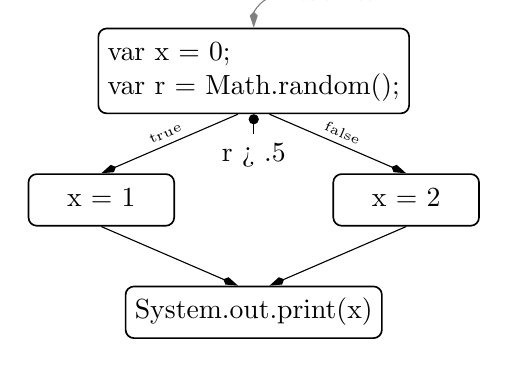
\begin{tikzpicture}[rect/.style={draw,rounded corners=3pt,semithick,rectangle,minimum width=1.85cm}]
   \node[rect,align=left] (bb1) at (0,0) {%
\strut\bjava{var x = 0;}\\
\bjava{var r = Math.random();}\strut
   };
   \node[below=2.5mm] (@bb1) at(bb1.south) {\bjava{r > .5}};
   \draw[-Circle] (@bb1) -- (bb1.south);
   \node[below left=7.5mm,xshift=-2.5mm,rect,align=left] (bb2) at(bb1.south) {
      \strut\bjava{x = 1}\strut
   };
   \node[below right=7.5mm,xshift=2.5mm,rect,align=left] (bb3) at(bb1.south) {
      \strut\bjava{x = 2}\strut
   };
   \node[below=7.5mm,rect,align=left] (bb4) at(current bounding box.south) {
      \strut\bjava{System.out.print(x)}\strut
   };
   \draw[-Kite] ([xshift=-2mm]bb1.south) to[edge node={node[above=-.35mm,sloped] {\tiny true}}] (bb2.north);
   \draw[-Kite] ([xshift=2mm]bb1.south) to[edge node={node[above=-.35mm,sloped] {\tiny false}}] (bb3.north);
   \draw[-Kite] (bb2.south) -- ([xshift=-2mm]bb4.north);
   \draw[-Kite] (bb3.south) -- ([xshift=2mm]bb4.north);
   \pgfinterruptboundingbox
   \onslide<22->{%
      \draw[Kite-,gray] (bb1.north) to[out=90,in=180] ++(3mm,4mm) node[bottom note,right] {Basic Block};
   }
   \endpgfinterruptboundingbox
\end{tikzpicture}
\end{lrbox}
\begin{lrbox}{\ExampleLivenessofCode}% beispiel wann es noch verwendet wird, unterschied zu scope was es live hält solange es sichtbar ist
\lstfs{8}
\begin{tikzpicture}[rect/.style={draw,rounded corners=3pt,semithick,rectangle,minimum width=1.85cm}]
   \node[rect,align=left] (bb1) at (0,0) {%
\strut\bjava{var x = 0;}\\
\bjava{var r = Math.random();}\strut
   };
   \node[below=2.5mm] (@bb1) at(bb1.south) {\bjava{r > .5}};
   \draw[-Circle] (@bb1) -- (bb1.south);
   \node[below left=7.5mm,xshift=-2.5mm,rect,align=left] (bb2) at(bb1.south) {
      \strut\bjava{x = 1}\strut
   };
   \node[below right=7.5mm,xshift=2.5mm,rect,align=left] (bb3) at(bb1.south) {
      \strut\bjava{x = 2}\strut
   };
   \node[below=7.5mm,rect,align=left] (bb4) at(current bounding box.south) {
      \strut\bjava{System.out.print(x)}\strut
   };
   \draw[-Kite] ([xshift=-2mm]bb1.south) to[edge node={node[above=-.35mm,sloped] {\tiny true}}] (bb2.north);
   \draw[-Kite] ([xshift=2mm]bb1.south) to[edge node={node[above=-.35mm,sloped] {\tiny false}}] (bb3.north);
   \draw[-Kite] (bb2.south) -- ([xshift=-2mm]bb4.north);
   \draw[-Kite] (bb3.south) -- ([xshift=2mm]bb4.north);
   \pgfinterruptboundingbox
   \foreach \i in {1,2,3,4} {
      \node[above left,yshift=-1mm,xshift=1.5pt] at(bb\i.north east) {\scriptsize b\i};
   }
   \endpgfinterruptboundingbox
   \onslide<25->{
      \fill[draw=black,thick,rounded corners=3pt,fill=white,fill opacity=.9,font=\small] (bb4.south west) rectangle (bb4.north east) node[midway,centered] {\(in_{b4} = \{\,x, \mathcolor{gray}{System.out.print}\,\}\)};
   }
   \onslide<26->{
      \fill[draw=black,thick,rounded corners=3pt,fill=white,fill opacity=.9,font=\small] (bb3.south west) rectangle (bb3.north east) node[midway,centered] {\(out_{b3} = \{\,x\,\}\)};
   }
   \onslide<27->{
      \fill[draw=black,thick,rounded corners=3pt,fill=white,fill opacity=.9,font=\small] (bb2.south west) rectangle (bb2.north east) node[midway,centered] {\(out_{b2} = \{\,x\,\}\)};
   }
   \onslide<28->{
      \fill[draw=black,thick,rounded corners=3pt,fill=white,fill opacity=.9,font=\small] (bb1.south west) rectangle (bb1.north east) node[midway,centered,align=center,text width=3cm] {\vspace*{-3.4mm}\begin{align*}
         in_{b1} &= \{\,\,\} \onslide<29->{~~\text{\scalebox{.75}{\color{gray}\faExclamationTriangle~see formula}}}\\
         out_{b1} &= \{\,\,\}
      \end{align*}}; % x, \;r not in out as they are not used afterward
   }
\end{tikzpicture}
\end{lrbox}
\begin{itemize}
   \itemsep4pt
   \item<2-> Support for multiple languages (15+)\medskip \begin{itemize}
      \itemsep4pt
      \item<3-> Widely varying \tikzmarknode{sonar-support}{support} and rules
      \item<5-> We focus on \tikzmarknode{sonar-java}{\href{https://github.com/SonarSource/sonar-java}{\textsb{sonar-java}}}\vspace*{-.55\baselineskip}
   \end{itemize}
   % use CFG, Ast visitor, own parser
   % TODO: extra features like magic comments as annotations etc. 
   \begin{tikzpicture}[overlay,remember picture]
      \onslide<4->{
         \draw[Kite-,gray] (sonar-support.south east) to[out=-20,in=180] ++(8mm,-1mm) node[right,bottom note] {Separate frontends and analyzers per language!};
      }
      \onslide<6->{
         \draw[Kite-,gray] ([yshift=1mm]sonar-java.south east) to[out=-30,in=180] ++(5mm,-1.33mm) node[right,bottom note] {704 rules!};
      }
   \end{tikzpicture}
\end{itemize}
\noindent
\begin{uncoverenv}<7->
\begin{lrbox}{\SonarLintShow}
\begin{tikzpicture}[o/.style={outer sep=0pt,inner sep=0pt},remember picture]
   \node[o] (@) at (0,0) {\usebox\CodeFile} coordinate (@code-file);
   \node[above=2.5mm,xshift=1.15mm,gray] at(@.north) {\textsb{\normalsize Input}};
\pgfonlayer{background}
\scope[transparency group,opacity=.4]
\node[o,rotate around={-30:(@.south east)},anchor=south east] at(@.south east) {\usebox\CodeFile};
\node[o,rotate around={-12:(@.south east)},anchor=south east] at(@.south east) {\usebox\CodeFile};
\endscope
\endpgfonlayer
\coordinate (@) at(@.east);
\foreach[count=\i] \usecase/\targeti in {{\raisebox{1pt}{Textual}}/1,Syntactical/0, Semantical/0, Historical/1, Annotated/0, {\raisebox{-3pt}{Metadata,~\ldots}}/1} { % program spectra, hardware, contexts, ...
\pgfmathsetmacro\rot{-24*\i+66}
      \path ([xshift=.5mm]@.east)++(\rot+10:1mm) coordinate (@a);
      \fill[opacity=.18,gray] (@a.east) -- ++(\rot:1.5cm) arc (\rot:\rot+20:1.5cm) -- cycle;
      \draw[thick,gray] (@a.east)++(\rot:1.5cm) arc (\rot:\rot+20:1.5cm);
      \tikzset{@/.style={}}
      \ifnum\targeti=1relax
         \only<9->{
            \tikzset{@/.style={opacity=.2}}
         }
      \fi
      \path (@a.east) -- ++(1.05*\rot+10:1.6cm) node[right,font=\small,darkgray,@] (@uc-\i) {\vphantom{a}\smash{\usecase}};
}
\coordinate (@east) at (current bounding box.east);
\onslide<10->{%
   \draw[decoration={brace},decorate,gray] ([yshift=.5mm]@uc-2.north east-|@uc-3.north east) -- ([yshift=-.5mm]@uc-3.south east) node[midway,right=1mm,font=\footnotesize,align=left] (jbc) {Read\,\&\,Process\\Java Bytecode}; % using java byte code is rather common
}
\node[above=1.65mm,xshift=1mm,gray] (persp) at(current bounding box.north) {\textsb{\normalsize Perspectives}};
\begin{onlyenv}<-7|handout:0>
\node[right,yshift=-7mm,xshift=1cm,align=left,font=\small,darkgray,text width=3.25cm] (@techn) at(@east){{{\subnode{tc-search}{Text/Code Search}\strut}}~\\[4mm]\strut{{\subnode{clustering}{Clustering}}}~\\[4mm]\strut{{\subnode{ai}{Abstract Domains}}}~\\[4mm]\strut{{\subnode{df-constraints}{Dataflow Constraints}}}~\\[1mm]\strut{{\centerline{\footnotesize\(\vdots\)}}}};
\node[above=1.5mm,gray,xshift=-4.5mm] at(@techn.north) {\textsb{\normalsize Theory}};
\scope[gray,line cap=round]
   \draw ([yshift=1.5pt]@uc-1.east) -- ([yshift=-2.5mm]@techn.north west);
   \draw ([yshift=1.5pt]@uc-2.east) -- ([yshift=-2.5mm]@techn.north west);
   \draw[densely dotted] ([yshift=1.5pt]@uc-3.east) -- ([yshift=-2.5mm]@techn.north west);
   \draw ([yshift=1.5pt]@uc-1.east) -- ([yshift=-10.5mm]@techn.north west);
   \draw ([yshift=0pt]@uc-2.east) -- ([yshift=-10.5mm]@techn.north west);
   \draw ([yshift=1.5pt]@uc-4.east) -- ([yshift=-10.5mm]@techn.north west);
   
   \draw ([yshift=-1pt]@uc-2.east) -- ([yshift=-18.5mm]@techn.north west);
   \draw ([yshift=-1pt]@uc-3.east) -- ([yshift=-18.5mm]@techn.north west);
   \draw ([yshift=1.5pt]@uc-5.east) -- ([yshift=-18.5mm]@techn.north west);
   
   \draw ([yshift=-1pt]@uc-2.east) -- ([yshift=-26mm]@techn.north west);
   \draw ([yshift=-1pt]@uc-3.east) -- ([yshift=-26mm]@techn.north west);
\endscope
   
   \node[right=7.5mm] (@) at(current bounding box.east) {\resizebox*!{2.85cm}{\usebox\UiBox}};
   \scope[transparency group,opacity=.5,every path/.append style={line cap=round,line width=.5pt}]
      \draw[-Kite,gray] ([yshift=-2.5mm,xshift=-6.5mm]@techn.north east) to[out=0,in=180] ([xshift=1.5mm,yshift=-6.35mm]@.west);
      \draw[-Kite,gray] ([yshift=-10.5mm,xshift=-18.5mm]@techn.north east) to[out=0,in=180] ([xshift=7.15mm,yshift=-1.35mm]@.west);
      \draw[-Kite,gray] ([yshift=-18.5mm,xshift=-6.25mm]@techn.north east) to[out=0,in=180] ([xshift=26.15mm,yshift=-9.35mm]@.west);
      \draw[-Kite,gray] ([yshift=-26mm,xshift=-2.5mm]@techn.north east) to[out=0,in=180] ([xshift=26.15mm,yshift=-9.35mm]@.west);
   \endscope
   \node[above, gray] at(@.north) {\tiny \textsb{\normalsize Communicate} or \textsb{\normalsize Use}};
\end{onlyenv}
\onslide<11->{%
   \draw[gray,-Kite] (@uc-5.east) to[out=0,in=180] ++(6.5mm,2mm) node[right,font=\footnotesize] {Ignore warnings,~\ldots};
}
\onslide<12->{%
   \draw[gray,Kite-] (jbc) to[out=80,in=260] ++(2mm,9mm) node[above,bottom note,align=center] {Java Compiler\\(Maven, Gradle,~\ldots)};
}
\onslide<13->{%
   \draw[gray,-Kite] ([xshift=-4.25mm]jbc.south) to[out=-80,in=180] ++(6mm,-3mm) node[right,bottom note,align=center] (dfg-cfg-note) {Calculate \subnode{cfg-analysis}{\link{https://github.com/SonarSource/sonar-java/blob/50b7d48e5764545a78a7ef2bf84b8a5ff1f30b3e/java-frontend/src/main/java/org/sonar/java/cfg/CFG.java\#L494}{CFG}}, \subnode{liveness-analysis}{\link{https://github.com/SonarSource/sonar-java/blob/50b7d48e5764545a78a7ef2bf84b8a5ff1f30b3e/java-frontend/src/main/java/org/sonar/java/cfg/LiveVariables.java\#L73}{Liveness}},~\ldots};
}
\onslide<14->{
   \node[above=3.5mm,gray,xshift=8.15mm] (theory) at(@techn.north) {\textsb{\normalsize Theory}};
}
\onslide<15->{
   \node[below=1mm] (dfg-constraints) at(theory.south) {\small Dataflow Constraints};
}
\onslide<16->{
   \draw[gray,-Kite] ([yshift=2mm,xshift=1.5mm]pic cs:cfg-analysis) to[out=90,in=250] ([xshift=-2mm]dfg-constraints.south);
}
\onslide<17->{
   \draw[gray,-Kite] ([xshift=2mm,xshift=1.5mm]dfg-constraints.south) to[out=290,in=80] ([yshift=2mm,xshift=1.5mm]pic cs:liveness-analysis);
}
\begin{uncoverenv}<31->
   \node[right=15.5mm,yshift=-.5mm,gray] (communicate) at(theory.east) {\textsb{\normalsize Communicate}};
   \node[below=1mm,draw=lightgray,thick,inner sep=0pt,opacity=.9] (sonar-com) at(communicate.south) {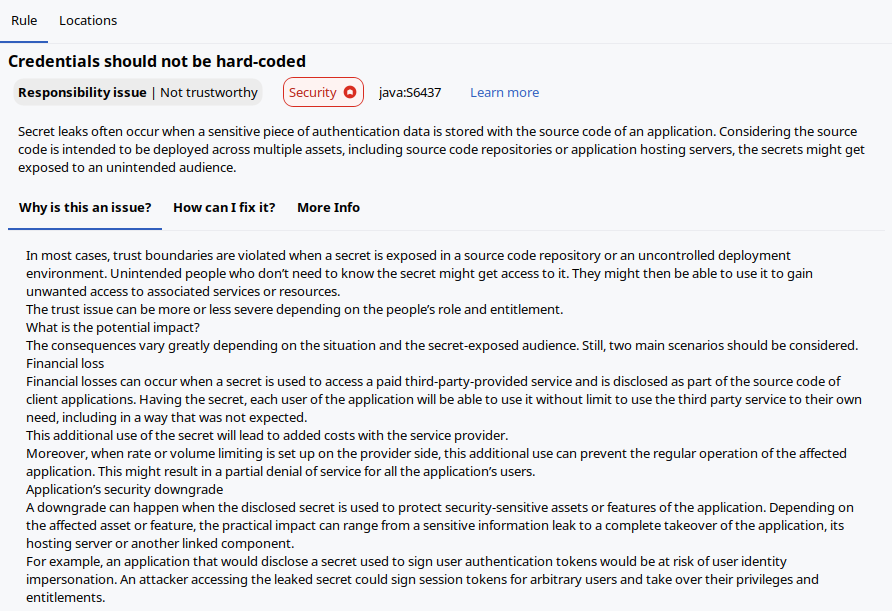
\includegraphics[width=3cm]{img/sonarlint-report.png}};
   \draw[gray,-Kite] ([xshift=6mm]dfg-constraints.south) to[out=-40,in=180] (sonar-com.west);
\end{uncoverenv}
\begin{onlyenv}<18-29|handout:2>
\onslide<18->{
   \pgfinterruptboundingbox
   \fill[white,fill opacity=.85] ([yshift=6mm]current page.south west) rectangle (current page.east|-persp.north);
   \endpgfinterruptboundingbox
   \node[draw=darkgray,fill=white,minimum width=4.2cm,minimum height=4.5cm,fill opacity=.93,rounded corners=3.45pt,thick,align=center,right] (@1) at ([xshift=-5mm,yshift=4mm]@code-file.west) {~\\[-5mm]{\onslide<19->{\usebox\ExampleCodeCfG}}};
   \node[above] at(@1.south) {\textsb{Code}};
}
\onslide<20->{
   \node[draw=darkgray,fill=white,minimum width=4cm,minimum height=4.5cm,fill opacity=.93,rounded corners=3.45pt,thick,right=7mm,align=center] (@2) at (@1.east) {%
   ~\\[-5mm]{\onslide<21->{\resizebox{4cm}!{\usebox\ExampleCFGofCode}}}%
   };
   \node[above] at(@2.south) {\textsb{Control Flow Graph}};
}
\onslide<23->{
   \node[draw=darkgray,fill=white,minimum width=4cm,minimum height=4.5cm,fill opacity=.93,rounded corners=3.45pt,thick,right=7mm,align=center] (@3) at (@2.east) {~\\[-5mm]{\onslide<24->{\resizebox{4cm}!{\usebox\ExampleLivenessofCode}}}};
   \pgfinterruptboundingbox
   \node[xshift=-12mm,yshift=4.2mm,draw=darkgray,fill=white,fill opacity=.93,rounded corners=3.45pt,thick,align=center,text width=4.5cm,scale=.65,font=\footnotesize,inner sep=1pt] at(@3.north east) {%
   \begin{align*}
      \mathbf{In}_n &= (\mathbf{Out}_n - \mathbf{Kill}_n) \cup \mathbf{Gen}_n \\
      \mathbf{Out}_n &= \begin{cases}
         \mathbf{BI} & n \text{~is End} \\
         \bigcup\limits_{m \in \text{succ}(n)} \mathbf{In}_m & \text{otherwise}
      \end{cases}
   \end{align*}
   With fixpoint iteration
   };
   \endpgfinterruptboundingbox
   \node[above] at(@3.south) {\textsb{Liveness}\textsuperscript{\smaller[2]\cite[p.\,26]{10.5555/1592955}}};
}
\end{onlyenv}
% by default iterated until reach fixpoint
\end{tikzpicture}
\end{lrbox}
\global\setbox\SonarLintShow=\copy\SonarLintShow
\begin{tikzpicture}[overlay,remember picture]
   \node[above=-1mm,xshift=.33mm] at(current page.south) {\usebox\SonarLintShow};
\end{tikzpicture}
\end{uncoverenv}
\begin{tikzpicture}[overlay,remember picture]
   \node[below left=4mm] at(current page.north east) {\Logo[2.5cm]{https://www.sonarsource.com/products/sonarlint/}{sonar}};
   \node[above right,yshift=4mm,bottom note] at(current page.south west) {\link{https://github.com/SonarSource}{github.com/SonarSource/sonar-java}};
   \only<23-|handout:2>{
      \node[above left,bottom note,yshift=4mm] at(current page.south east) {\cite{10.5555/1592955}~\citetitle{10.5555/1592955} (\citeauthor{10.5555/1592955})};
   }
\end{tikzpicture}
\end{frame}

\lstfs{11}
\begin{frame}[t,fragile]{\textcolor{gray}{SonarLint ---~}Unused Assignments}
\begin{itemize}
   \itemsep9pt
   \item<2-> Analyze \enquote{Dead Stores} {\onslide<3->{\smaller[2]\textcolor{gray}{(in 311\,loc\,/\,259\,cloc)}:}}
\begin{minted}[escapeinside=||]{java}
|\onslide<4->|int x = 0;
x = 42;|\onslide<1->|
\end{minted}
   \item<5-> Use \link{https://github.com/SonarSource/sonar-java/blob/50b7d48e5764545a78a7ef2bf84b8a5ff1f30b3e/java-frontend/src/main/java/org/sonar/java/cfg/LiveVariables.java\#L73}{liveness analysis} to obtain \(out_n\) of each basic block in the CFG
   \item<6-> Check if assignments (\bjava{x =}, \bjava{x++},~\ldots) are in \(out_n\) and resolved
   \item<7-> Check overwrites in the same basic block
   \item<8-> Minor special handling for \bjava{try-finally} blocks,~\ldots
\end{itemize}
\begin{tikzpicture}[overlay,remember picture]
   \node[below left=4mm] at(current page.north east) {\Logo[2.5cm]{https://www.sonarsource.com/products/sonarlint/}{sonar}};
   \node[above right,bottom note, yshift=4mm] at(current page.south west) {\link{https://github.com/SonarSource/sonar-java/blob/50b7d48e5764545a78a7ef2bf84b8a5ff1f30b3e/java-checks/src/main/java/org/sonar/java/checks/DeadStoreCheck.java\#L52}{Implementation of Rule S1854}};
   \begin{uncoverenv}<9-|handout:2>
      \xlstsetmintedstyle{plain number}
      \node[above left=2mm,yshift=5.5mm,text width=.75\paperwidth,fill=white,draw,rounded corners=3pt,inner ysep=0pt,fill opacity=.95,drop shadow={fill=lightgray!50}] at(current page.south east) {\lstfs{8}%
\begin{minted}[firstnumber=77,morekeywords={[3]{CFG,Block,LiveVariables}},xleftmargin=7mm,prebreak={}]{java}
LiveVariables liveVariables = LiveVariables.analyze(cfg);
// Liveness analysis provides information only for block boundaries, so we should do analysis between elements within blocks
for(CFG.Block block : cfg.blocks()) {
   checkElements(block, liveVariables.getOut(block), methodSymbol);
}
\end{minted}
      };
   \end{uncoverenv}
\end{tikzpicture}
\end{frame}


\begin{frame}[t,fragile]{\textcolor{gray}{SonarLint ---~}Hardcoded Credentials}
\begin{itemize}
   \itemsep8pt
   \item<2-> It does not always have to be that heavy! {\onslide<3->{\smaller[2]\textcolor{gray}{(116\,loc\,/\,87\,cloc may suffice)}}}
   \item<4-> For example, to identify hardcoded credentials:
{%
\lstfs{9}
\begin{minted}[escapeinside=||]{java}
|\onslide<5->|new PasswordAuthentication("password", "secret".toCharArray());|\onslide<1->|
\end{minted}
}\vspace*{-.85\baselineskip}
   \item<6-> Traverse the Abstract Syntax Tree~(AST)
   \item<7-> Check calls against a long \link{https://github.com/SonarSource/sonar-java/blob/3e2cb4478100a5ea082dde30004067579eef58a4/java-checks-aws/src/main/resources/org/sonar/java/checks/security/S6437-methods.json}{list of signatures} (currently 7664) with problematic indices
   \item<8-> Check if the arguments are \enquote{constant}\\
   \onslide<9->{\textcolor{gray}{visiting the dataflow links and checking for predefined \enquote{plain text}}}
\end{itemize}
\begin{tikzpicture}[overlay,remember picture]
   \node[below left=4mm] at(current page.north east) {\Logo[2.5cm]{https://www.sonarsource.com/products/sonarlint/}{sonar}};
   \node[above right,bottom note, yshift=4mm] at(current page.south west) {\link{https://github.com/SonarSource/sonar-java/blob/50b7d48e5764545a78a7ef2bf84b8a5ff1f30b3e/java-checks-aws/src/main/java/org/sonar/java/checks/security/HardCodedCredentialsShouldNotBeUsedCheck.java\#L43}{Implementation of Rule S6437}};
   % TODO: mark heuristics: list of signatures and constant check
   \begin{uncoverenv}<10-|handout:2>
      \xlstsetmintedstyle{plain number}
      % \xlstblacklistlinenumbers{111}
      \node[above left=2mm,yshift=5.5mm,text width=.9\paperwidth,fill=white,draw,rounded corners=3pt,inner ysep=0pt,fill opacity=.95,drop shadow={fill=lightgray!50}] at(current page.south east) {\lstfs{8}%
\begin{minted}[firstnumber=107,morekeywords={[3]{ExpressionTree,JavaFileScannerContext,Location,ISSUE_MESSAGE}},xleftmargin=7mm,prebreak={}]{java}
for (int targetArgumentIndex : method.indices) {
   ExpressionTree argument = arguments.get(targetArgumentIndex);
   var secondaryLocations = new ArrayList<JavaFileScannerContext.Location>();
   if (isExpressionDerivedFromPlainText(argument, secondaryLocations, new HashSet<>())) {
      reportIssue(argument, ISSUE_MESSAGE, secondaryLocations, null);
   }
}
\end{minted}
      };
   \end{uncoverenv}
\end{tikzpicture}
\end{frame}


\subsection{Astrée}
\againframe<0,7,17|handout:3>{tool-slide}
\begin{frame}{Astrée}
   \begin{itemize}
      \itemsep4.5pt
      \item<2-> \textit{Analyseur statique de logiciels temps-réel embarqués}\\\textcolor{gray}{Static analyzer for real-time embedded software}
      \item<3-> Proprietary, sound\only<4->{\textcolor{gray}{\textit{y}}} static analyzer for \tikzmarknode{astree-features}{C/C++}
      \item<6-> Uses abstract domains for timing validation, buffer overflows,~\ldots
   \end{itemize}
\begin{uncoverenv}<7->
\begin{tikzpicture}[o/.style={outer sep=0pt,inner sep=0pt},remember picture]
   \node[o] (@) at (0,0) {\usebox\CodeFile};
   \node[above=2.5mm,xshift=1.15mm,gray] at(@.north) {\textsb{\normalsize Input}};
\pgfonlayer{background}
\scope[transparency group,opacity=.4]
\node[o,rotate around={-30:(@.south east)},anchor=south east] at(@.south east) {\usebox\CodeFile};
\node[o,rotate around={-12:(@.south east)},anchor=south east] at(@.south east) {\usebox\CodeFile};
\endscope
\endpgfonlayer
\coordinate (@) at(@.east);
\foreach[count=\i] \usecase/\targeti in {{\raisebox{1pt}{Textual}}/0,Syntactical/0, Semantical/0, Historical/1, Annotated/0, {\raisebox{-3pt}{Metadata,~\ldots}}/1} { % program spectra, hardware, contexts, ...
\pgfmathsetmacro\rot{-24*\i+66}
      \path ([xshift=.5mm]@.east)++(\rot+10:1mm) coordinate (@a);
      \fill[opacity=.18,gray] (@a.east) -- ++(\rot:1.5cm) arc (\rot:\rot+20:1.5cm) -- cycle;
      \draw[thick,gray] (@a.east)++(\rot:1.5cm) arc (\rot:\rot+20:1.5cm);
      \tikzset{@/.style={}}
      \ifnum\targeti=1relax
         \only<9->{
            \tikzset{@/.style={opacity=.2}}
         }
      \fi
      \path (@a.east) -- ++(1.05*\rot+10:1.6cm) node[right,font=\small,darkgray,@] (@uc-\i) {\vphantom{a}\smash{\usecase}};
}
\coordinate (@east) at (current bounding box.east);
\onslide<10->{%
   \draw[decoration={brace},decorate,gray] ([yshift=.5mm]@uc-1.north east-|@uc-3.north east) -- ([yshift=-.5mm]@uc-3.south east) node[midway,right=1mm,font=\footnotesize,align=left] (jbc) {Build abstractions\\handle undef. behavior}; % using java byte code is rather common
}
\node[above=1.65mm,xshift=1mm,gray] at(current bounding box.north) {\textsb{\normalsize Perspectives}};
\begin{onlyenv}<-7|handout:0>
\node[right,yshift=-7mm,xshift=1cm,align=left,font=\small,darkgray,text width=3.25cm] (@techn) at(@east){{{{Text/Code Search}\strut}}~\\[4mm]\strut{{{Clustering}}}~\\[4mm]\strut{{{Abstract Domains}}}~\\[4mm]\strut{{{Dataflow Constraints}}}~\\[1mm]\strut{{\centerline{\footnotesize\(\vdots\)}}}};
\node[above=1.5mm,gray,xshift=-4.5mm] at(@techn.north) {\textsb{\normalsize Theory}};
\scope[gray,line cap=round]
   \draw ([yshift=1.5pt]@uc-1.east) -- ([yshift=-2.5mm]@techn.north west);
   \draw ([yshift=1.5pt]@uc-2.east) -- ([yshift=-2.5mm]@techn.north west);
   \draw[densely dotted] ([yshift=1.5pt]@uc-3.east) -- ([yshift=-2.5mm]@techn.north west);
   \draw ([yshift=1.5pt]@uc-1.east) -- ([yshift=-10.5mm]@techn.north west);
   \draw ([yshift=0pt]@uc-2.east) -- ([yshift=-10.5mm]@techn.north west);
   \draw ([yshift=1.5pt]@uc-4.east) -- ([yshift=-10.5mm]@techn.north west);
   
   \draw ([yshift=-1pt]@uc-2.east) -- ([yshift=-18.5mm]@techn.north west);
   \draw ([yshift=-1pt]@uc-3.east) -- ([yshift=-18.5mm]@techn.north west);
   \draw ([yshift=1.5pt]@uc-5.east) -- ([yshift=-18.5mm]@techn.north west);
   
   \draw ([yshift=-1pt]@uc-2.east) -- ([yshift=-26mm]@techn.north west);
   \draw ([yshift=-1pt]@uc-3.east) -- ([yshift=-26mm]@techn.north west);
\endscope
   
   \node[right=7.5mm] (@) at(current bounding box.east) {\resizebox*!{2.85cm}{\usebox\UiBox}};
   \scope[transparency group,opacity=.5,every path/.append style={line cap=round,line width=.5pt}]
      \draw[-Kite,gray] ([yshift=-2.5mm,xshift=-6.5mm]@techn.north east) to[out=0,in=180] ([xshift=1.5mm,yshift=-6.35mm]@.west);
      \draw[-Kite,gray] ([yshift=-10.5mm,xshift=-18.5mm]@techn.north east) to[out=0,in=180] ([xshift=7.15mm,yshift=-1.35mm]@.west);
      \draw[-Kite,gray] ([yshift=-18.5mm,xshift=-6.25mm]@techn.north east) to[out=0,in=180] ([xshift=26.15mm,yshift=-9.35mm]@.west);
      \draw[-Kite,gray] ([yshift=-26mm,xshift=-2.5mm]@techn.north east) to[out=0,in=180] ([xshift=26.15mm,yshift=-9.35mm]@.west);
   \endscope
   \node[above, gray] at(@.north) {\tiny \textsb{\normalsize Communicate} or \textsb{\normalsize Use}};
\end{onlyenv}
\onslide<11->{%
   \draw[gray,-Kite] (@uc-5.east) to[out=0,in=180] ++(6.5mm,2mm) node[below right,font=\footnotesize,yshift=.7\baselineskip,align=left] {Specifications, Configuration,~\ldots\\for widening, assumptions,~\ldots};
}
\onslide<12->{%
   \draw[gray,Kite-] (jbc) to[out=80,in=260] ++(2mm,9mm) node[above,bottom note,align=center] {C/C++ Project};
}
\onslide<13->{%
   \draw[gray,-Kite] ([xshift=-4.25mm]jbc.south) to[out=-80,in=180] ++(6mm,-3mm) node[right,bottom note,align=center] (cfg-dr-note) {CFG, Data Races,~\ldots};
}
\onslide<14->{
   \node[above=3.5mm,gray,xshift=20.5mm] (theory) at(@techn.north) {\textsb{\normalsize Theory}};
}
\onslide<15->{
   \node[below=1mm,align=right] (a-domains) at(theory.south) {\small Abstract Domains\\[-1mm]\footnotesize\textcolor{gray}{\(\approx30\)}}; % many parameterized
}
\onslide<16->{
   \draw[gray,Kite-Kite] ([yshift=4mm]a-domains.south) to[bend left] (cfg-dr-note.east);
}
\begin{uncoverenv}<17->
   \node[right=17.5mm,yshift=-.5mm,gray] (communicate) at(theory.east) {\textsb{\normalsize Communicate}};
   \node[below=1mm,draw=lightgray,thick,inner sep=0pt,opacity=.9] (astree-com) at(communicate.south) {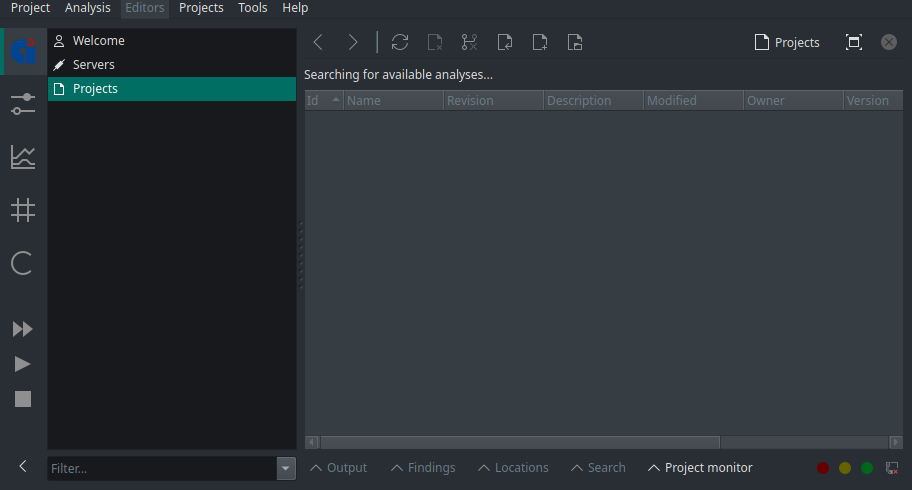
\includegraphics[width=3cm]{img/astree-report.png}};
   \draw[gray,-Kite] ([yshift=3.8mm,xshift=1mm]a-domains.south) to[out=-40,in=180] (astree-com.west);
\end{uncoverenv}
\end{tikzpicture}
\end{uncoverenv}
   \begin{tikzpicture}[overlay,remember picture]
      \node[below left=4mm] at(current page.north east) {\Logo[26.25mm]{https://www.absint.com/astree/index.htm}{astree}};
      \onslide<5->{
         % 100+ directives and intrinsics, 140+ options
         \draw[-Kite,gray] (astree-features.east) to[out=20,in=180] ++(6mm,2mm) node[right,bottom note,align=left] {100+ directives and intrinsics, 140+ options\\250\,kloc of Ocaml, 240\,kloc C/C++};
      }
      \onslide<18->{
         \node[above left,yshift=5mm,xshift=-2mm,align=center] (antime) at(current page.south east) {Analysis Time\\[-.5mm]\color{gray}\scriptsize from couple of hours to days};
      }
      \onslide<19->{
         \draw[gray,Kite-] ([xshift=4mm,yshift=-2mm]antime.north west) to[out=110,in=-20] ++(-5.65mm,4mm) node[left,bottom note] {Local precision tuning};
      }
      \onslide<20->{
         \draw[gray,Kite-] ([xshift=4mm,yshift=.5mm]antime.north) to[out=120,in=-20] ++(-5.65mm,4mm) node[left,bottom note] {Semantic Loop Unrolling}; % based on relevance, ...
      }
      \onslide<21->{
         \draw[gray,Kite-] ([xshift=2mm,yshift=.5mm]antime.west) to[out=150,in=-10] ++(-5.65mm,2mm) node[left,bottom note] {Interleaving Semantics}; % parallel code, ...
      }
   \end{tikzpicture}
\end{frame}

\newsavebox\pinguLook
\savebox\pinguLook{\scalebox{.65}{\tikz{\pingu[left eye wink,right wing wave,magnifier right,small,tie,deer hat]}}} 

\subsection{LiSA}
\againframe<7,18|handout:4>{tool-slide}
\begin{frame}{LiSA}
\begin{itemize}
   \itemsep6.5pt
   \item<2-> \textcolor{gray}{(Largely)} Language Independent \underline{Li}brary for \underline{S}tatic \tikzmarknode{lisa-alts}{\underline{A}nalysis}
   \item<4-> Custom frontends for Rust, Go, Python, EVM,~\ldots
\end{itemize}
\begin{tikzpicture}[overlay,remember picture]
   \node[below left=4mm] at(current page.north east) {\Logo[2cm]{https://github.com/lisa-analyzer/lisa}{lisa}};
   \node[above right,yshift=4mm,bottom note] at(current page.south west) {\link{https://github.com/lisa-analyzer/lisa}{github.com/lisa-analyzer/lisa}};
   \onslide<3->{%
      \draw[-Kite,gray] ([xshift=1.5mm]lisa-alts.east) to[out=0,in=180] ++(6mm,2mm) node[right,bottom note,align=left] {Similar to \link{https://mopsa.lip6.fr/}{Mopsa} or \link{https://github.com/antoinemine/apron}{Apron}};
   }
\end{tikzpicture}
\begin{uncoverenv}<5->
\begin{tikzpicture}[o/.style={outer sep=0pt,inner sep=0pt},remember picture]
   \node[o] (@) at (0,0) {\usebox\CodeFile};
   \node[above=2.5mm,xshift=1.15mm,gray] at(@.north) {\textsb{\normalsize Input}};
\pgfonlayer{background}
\scope[transparency group,opacity=.4]
\node[o,rotate around={-30:(@.south east)},anchor=south east] at(@.south east) {\usebox\CodeFile};
\node[o,rotate around={-12:(@.south east)},anchor=south east] at(@.south east) {\usebox\CodeFile};
\endscope
\endpgfonlayer
\coordinate (@) at(@.east);
\foreach[count=\i] \usecase/\targeti in {{\raisebox{1pt}{Textual}}/1,Syntactical/0, Semantical/0, Historical/1, Annotated/0, {\raisebox{-3pt}{Metadata,~\ldots}}/1} { % program spectra, hardware, contexts, ...
\pgfmathsetmacro\rot{-24*\i+66}
      \path ([xshift=.5mm]@.east)++(\rot+10:1mm) coordinate (@a);
      \fill[opacity=.18,gray] (@a.east) -- ++(\rot:1.5cm) arc (\rot:\rot+20:1.5cm) -- cycle;
      \draw[thick,gray] (@a.east)++(\rot:1.5cm) arc (\rot:\rot+20:1.5cm);
      \tikzset{@/.style={}}
      \ifnum\targeti=1relax
         \only<7->{
            \tikzset{@/.style={opacity=.2}}
         }
      \fi
      \path (@a.east) -- ++(1.05*\rot+10:1.6cm) node[right,font=\small,darkgray,@] (@uc-\i) {\vphantom{a}\smash{\usecase}};
}
\coordinate (@east) at (current bounding box.east);
\onslide<8->{%
   \draw[decoration={brace},decorate,gray] ([yshift=.5mm]@uc-2.north east-|@uc-3.north east) -- ([yshift=-.5mm]@uc-3.south east) node[midway,right=1mm,font=\footnotesize,align=left] (jbc) {Construct CFG}; % using java byte code is rather common
}
\node[above=1.65mm,xshift=1mm,gray] at(current bounding box.north) {\textsb{\normalsize Perspectives}};
\begin{onlyenv}<-5|handout:0>
\node[right,yshift=-7mm,xshift=1cm,align=left,font=\small,darkgray,text width=3.25cm] (@techn) at(@east){{{{Text/Code Search}\strut}}~\\[4mm]\strut{{{Clustering}}}~\\[4mm]\strut{{{Abstract Domains}}}~\\[4mm]\strut{{{Dataflow Constraints}}}~\\[1mm]\strut{{\centerline{\footnotesize\(\vdots\)}}}};
\node[above=1.5mm,gray,xshift=-4.5mm] at(@techn.north) {\textsb{\normalsize Theory}};
\scope[gray,line cap=round]
   \draw ([yshift=1.5pt]@uc-1.east) -- ([yshift=-2.5mm]@techn.north west);
   \draw ([yshift=1.5pt]@uc-2.east) -- ([yshift=-2.5mm]@techn.north west);
   \draw[densely dotted] ([yshift=1.5pt]@uc-3.east) -- ([yshift=-2.5mm]@techn.north west);
   \draw ([yshift=1.5pt]@uc-1.east) -- ([yshift=-10.5mm]@techn.north west);
   \draw ([yshift=0pt]@uc-2.east) -- ([yshift=-10.5mm]@techn.north west);
   \draw ([yshift=1.5pt]@uc-4.east) -- ([yshift=-10.5mm]@techn.north west);
   
   \draw ([yshift=-1pt]@uc-2.east) -- ([yshift=-18.5mm]@techn.north west);
   \draw ([yshift=-1pt]@uc-3.east) -- ([yshift=-18.5mm]@techn.north west);
   \draw ([yshift=1.5pt]@uc-5.east) -- ([yshift=-18.5mm]@techn.north west);
   
   \draw ([yshift=-1pt]@uc-2.east) -- ([yshift=-26mm]@techn.north west);
   \draw ([yshift=-1pt]@uc-3.east) -- ([yshift=-26mm]@techn.north west);
\endscope
   
   \node[right=7.5mm] (@) at(current bounding box.east) {\resizebox*!{2.85cm}{\usebox\UiBox}};
   \scope[transparency group,opacity=.5,every path/.append style={line cap=round,line width=.5pt}]
      \draw[-Kite,gray] ([yshift=-2.5mm,xshift=-6.5mm]@techn.north east) to[out=0,in=180] ([xshift=1.5mm,yshift=-6.35mm]@.west);
      \draw[-Kite,gray] ([yshift=-10.5mm,xshift=-18.5mm]@techn.north east) to[out=0,in=180] ([xshift=7.15mm,yshift=-1.35mm]@.west);
      \draw[-Kite,gray] ([yshift=-18.5mm,xshift=-6.25mm]@techn.north east) to[out=0,in=180] ([xshift=26.15mm,yshift=-9.35mm]@.west);
      \draw[-Kite,gray] ([yshift=-26mm,xshift=-2.5mm]@techn.north east) to[out=0,in=180] ([xshift=26.15mm,yshift=-9.35mm]@.west);
   \endscope
   \node[above, gray] at(@.north) {\tiny \textsb{\normalsize Communicate} or \textsb{\normalsize Use}};
\end{onlyenv}
\onslide<9->{%
   \draw[gray,-Kite] (@uc-5.east) to[out=0,in=180] ++(6.5mm,2mm) node[below right,font=\footnotesize,yshift=.7\baselineskip,align=left] {(Depends on Frontend)};
}
\onslide<10->{%
   \draw[gray,Kite-] (jbc) to[out=80,in=260] ++(2mm,7.5mm) node[above,bottom note,align=center] {Language-Specific\\Frontends};
}
\onslide<11->{%
   \draw[gray,-Kite] ([xshift=-4.25mm]jbc.south) to[out=-80,in=180] ++(6mm,-3mm) node[right,bottom note,align=center] (cfg-dr-note) {\link{https://github.com/lisa-analyzer/lisa/blob/2543b47cfdb0a968a064d16f000fa0ad1d823125/lisa/lisa-analyses/src/main/java/it/unive/lisa/analysis/dataflow/Liveness.java\#L25}{Liveness}, \link{https://github.com/lisa-analyzer/lisa/blob/cd351110a5c47f69a16f0ca025058ad5a53976cb/lisa/lisa-analyses/src/main/java/it/unive/lisa/analysis/numeric/Pentagon.java\#L47}{Pentagons},~\ldots};
}
\onslide<12->{
   \node[above=3.5mm,gray,xshift=20.5mm] (theory) at(@techn.north) {\textsb{\normalsize Theory}};
}
\onslide<13->{
   \node[below=1mm,align=right] (a-domains) at(theory.south) {\small Abstract Domains}; % many parameterized
}
\onslide<14->{
   \draw[gray,Kite-Kite] (a-domains.south) to[bend left] (cfg-dr-note.east);
}
\begin{uncoverenv}<15->
   \node[right=20.5mm,yshift=-.5mm,gray] (communicate) at(theory.east) {\textsb{\normalsize Use}};
   \node[below=1mm,thick,inner sep=0pt,align=center,font=\small] (lisa-use) at(communicate.south) {Extension Interfaces\\Fixpoint Iterations,\\\ldots};
   \draw[gray,-Kite] ([xshift=1mm]a-domains.south) to[out=-40,in=180] (lisa-use.west);
\end{uncoverenv}
\onslide<16->{%
   \node[above left=2mm,yshift=3mm] (@ping) at(current page.south east) {\usebox\pinguLook};
   \node[left,gray,align=right] at(@ping.west) {Let's have a\\closer look!};
}
\end{tikzpicture}
\end{uncoverenv}
\end{frame}

\newsavebox\IntervalLattice
\begin{lrbox}{\IntervalLattice}
\scriptsize
\begin{tikzpicture}[line cap=round,x=6.5mm,y=6.5mm,gray]
   \matrix (A) [matrix of nodes, row sep=2.5mm, column sep=-2mm]
   {
       & &  & \I{-1}{\infty} & & & \\
       & & \I{-1}{1} & \ldots & \I{0}{2} & & \\
      & \I{-1}{0} & \ldots & \I01 & \ldots & \I{1}{2} & \\
      \I{-1}{-1} & \ldots & \I00 & \ldots & \I11 & \ldots & \I22 \\
      & & & \absexpr{\bot} & & & \\
   };
   \scope[line cap=round]
   \draw (A-2-3) -- (A-3-2) -- (A-4-1) -- (A-5-4);
   \draw (A-3-6) -- (A-4-7) -- (A-5-4);
   \draw (A-3-2) -- (A-4-3) -- (A-3-4) (A-3-4) -- (A-4-5) -- (A-3-6);
   \draw (A-2-3) -- (A-3-4) (A-3-4) -- (A-2-5) -- (A-3-6);
   \draw (A-4-3) -- (A-5-4) -- (A-4-5);
   \draw[densely dotted] (A-2-5) -- (A-1-4) -- (A-2-3);
   \draw[densely dotted] (A-5-4) -- ++(-1,0.05)  (A-5-4) -- ++(1,0.05);
   \foreach[count=\y] \i in {4,3,2,1} {
      \draw[densely dotted] (A-\y-\i.north west) -- ++(-.4,0.14);
      \node[left=3.5mm] at(A-\y-\i.west) {\footnotesize\ldots};
      \pgfmathsetmacro\other{int(8-\i)}
      \draw[densely dotted] (A-\y-\other.north east) -- ++(.4,0.14);
      \node[right=3.5mm] at(A-\y-\other.east) {\footnotesize\ldots};
   }
   \node[above=3.5mm] (pz) at(A-1-4.north) {\absexpr{\top}};
   \draw[densely dotted] (pz) -- ++(-1.25,-0.1) (pz) -- ++(1.25,-0.1);
   \endscope
\end{tikzpicture}
\end{lrbox}

\makeatletter
% https://github.com/lisa-analyzer/lisa/blob/bd00779ab87e1cd31ed01b97d9b0e71b922f5bcf/lisa/lisa-analyses/src/main/java/it/unive/lisa/analysis/numeric/Interval.java#L47
\def\FakeLineNumber#1{\llap{\xlstGetStyle{linenumbers}\href{https://github.com/lisa-analyzer/lisa/blob/bd00779ab87e1cd31ed01b97d9b0e71b922f5bcf/lisa/lisa-analyses/src/main/java/it/unive/lisa/analysis/numeric/Interval.java\#L#1}{\underline{\xlst@lst@num@consume{#1}}}~~~}}

\begin{frame}[fragile]{\textcolor{gray}{LiSA ---~}Interval Analysis\textsuperscript{\color{gray}\smaller[2]\cite[p.\,389]{cousout2021principles}}}
\lstfs{8}
\begin{uncoverenv}<7->
{\scriptsize\color{gray}\link{https://github.com/lisa-analyzer/lisa/blob/bd00779ab87e1cd31ed01b97d9b0e71b922f5bcf/lisa/lisa-analyses/src/main/java/it/unive/lisa/analysis/numeric/Interval.java}{\hbox{\faFileCodeO~}lisa-analyses/src/main/java/it/unive/lisa/analysis/numeric/Interval.java} (simplified)}
\AnimateCode{onslide={o1:{2},-,o3:{4,...,7},o8:{9,...,13},-,0,-},first slide=7,handout=12/1}
\begin{minted}[morekeywords={Interval,IntInterval,Constant,ProgramPoint,SemanticOracle,SemanticException},escapeinside=||]{java}
|\FakeLineNumber{57}|Interval TOP = new Interval(IntInterval.INFINITY);
|\onslide<8->{\FakeLineNumber{62}}\onslide<8->|Interval BOTTOM = new Interval(null);|\medskip|
|\onslide<9->{\FakeLineNumber{273}}\onslide<9->|public Interval lubAux(Interval other) {
|\onslide<9->{\FakeLineNumber{276}}\onslide<9->|   var newL = getLow().min(other.getLow());
|\onslide<9->{\FakeLineNumber{277}}\onslide<9->|   var newH = getHigh().max(other.getHigh());
|\onslide<9->{\FakeLineNumber{278}}\onslide<9->|   return new Interval(newLow, newHigh);
|\onslide<9->{\FakeLineNumber{279}}\onslide<9->|}|\medskip\onslide<1->|
|\onslide<10->{\FakeLineNumber{282}}\onslide<10->|public Interval glbAux(Interval other) {
|\onslide<10->{\FakeLineNumber{284}}\onslide<10->|   var newL = getLow().max(other.getLow());
|\onslide<10->{\FakeLineNumber{285}}\onslide<10->|   var newH = getHigh().min(other.getHigh());|\onslide<1->|
|\onslide<10->{\FakeLineNumber{287}}\onslide<11->|   if(newLow.compareTo(newHigh) > 0) return bottom();
|\onslide<11->{\FakeLineNumber{289}}\onslide<10->|   return new Interval(newLow, newHigh);
|\onslide<10->{\FakeLineNumber{290}}\onslide<10->|}|\vspace*{-5mm}\onslide<1->|
\end{minted}
\endAnimateCode
\onslide<12->{\footnotesize\textit{Widening, Narrowing, Assume, Satisfies,~\ldots}}
\end{uncoverenv}
\begin{tikzpicture}[overlay,remember picture]
   \node[above right,yshift=4mm,bottom note] at(current page.south west) {\cite{cousout2021principles}~\citetitle{cousout2021principles} (\citeauthor{cousout2021principles})};
   \onslide<2->{\node[above left,yshift=5mm,scale=.8] (int-latt) at(current page.south east) {\usebox\IntervalLattice};}
   \onslide<3->{%
      \node[above,text width=5cm,font=\scriptsize] at(int-latt.north) {%
         \begin{align*}
            \top &= \I{-\infty}{\infty} \tag*{Top}\\
            \onslide<4->{\bot} &\onslide<4->{{}= \absexpr{\emptyset} \only<4->{\tag*{Bottom}}} \\
            \onslide<5->{\absexpr{\Lub_{k}} \I{\ell_k}{h_k}} &\onslide<5->{{}=\I{\min(\ell_k)}{\max(h_k)} \only<5->{\tag*{Join}}} \\
            \onslide<6->{\absexpr{\Glb_{k}} \I{\ell_k}{h_k}} &\onslide<6->{{}=\I{\max(\ell_k)}{\min(h_k)} \only<6->{\tag*{Meet}}}
            % hidden for now
            % \I{\ell_l}{h_l} \absexpr{\widen} \I{\ell_r}{h_r} &= \I{\ell_l > \ell_r ? -\infty : \ell_l}{h_l < h_r ? \infty : h_l} \tag*{Widening}
         \end{align*}
      };
   }
\end{tikzpicture}
\end{frame}

\begin{frame}[fragile]{\textcolor{gray}{LiSA ---~}Interval Analysis\textsuperscript{\color{gray}\smaller[2]\cite[p.\,389]{cousout2021principles}}\hfill Semantics}
\lstfs{8}
\onslide<2->{When to create which interval?}\\*
\begin{uncoverenv}<3->
{\scriptsize\color{gray}\link{https://github.com/lisa-analyzer/lisa/blob/bd00779ab87e1cd31ed01b97d9b0e71b922f5bcf/lisa/lisa-analyses/src/main/java/it/unive/lisa/analysis/numeric/Interval.java}{\hbox{\faFileCodeO~}lisa-analyses/src/main/java/it/unive/lisa/analysis/numeric/Interval.java} (simplified)}
\AnimateCode{onslide={o1:{3,...,8},-,-,o9:{10},o11:{12},o1:{3,...,12},-},first slide=3,handout=8/1}
\preto\ldots{\color{lightgray}}% hijack the literate
\begin{minted}[morekeywords={Interval,IntInterval,Constant,ProgramPoint,SemanticOracle,SemanticException},escapeinside=||]{java}
|\onslide<3->{\FakeLineNumber{144}}\onslide<3->|public Interval evalNonNullConstant(Constant constant,
|\onslide<3->{\FakeLineNumber{146}}\onslide<3->|      ProgramPoint pp, SemanticOracle oracle) {
|\onslide<4->{\FakeLineNumber{148}}\onslide<4->|   if(constant.getValue() instanceof Integer) {
|\onslide<4->{\FakeLineNumber{149}}\onslide<4->|      var i = (Integer) constant.getValue();
|\onslide<4->{\FakeLineNumber{150}}\onslide<4->|      return new Interval(i, i);
|\onslide<4->{\FakeLineNumber{151}}\onslide<4->|   }
|\onslide<5->{\FakeLineNumber{152}}\onslide<5->|   return top();|\onslide<1->|
|\onslide<3->{\FakeLineNumber{153}}\onslide<3->|}|\medskip\onslide<1->|
|\onslide<6->{\FakeLineNumber{157}}\onslide<6->|public Interval evalUnaryExpression(UnaryOperator op,
|\onslide<6->{\FakeLineNumber{158}}|    Interval arg, :ldots:) { :ldots: }|\onslide<1->|
|\onslide<7->{\FakeLineNumber{188}}\onslide<7->|public Interval evalBinaryExpression(BinaryOperator op,
|\onslide<7->{\FakeLineNumber{189}}|    Interval left, |\tikzmarknode{fold-like-marker}{\strut}|Interval right, :ldots:) { :ldots: }|\onslide<1->|
\end{minted}
\endAnimateCode
\end{uncoverenv}
\begin{tikzpicture}[overlay,remember picture]
   \node[above right,yshift=4mm,bottom note] at(current page.south west) {\cite{cousout2021principles}~\citetitle{cousout2021principles} (\citeauthor{cousout2021principles})};
   \node[above left,yshift=5mm,scale=.8] (int-latt) at(current page.south east) {\usebox\IntervalLattice};
   \onslide<9->{%
      \coordinate (@) at(fold-like-marker);
      \draw[Kite-,gray] ([xshift=5mm,yshift=-1mm]@) to[out=280,in=180] ++(3mm,-4mm) node[right,bottom note] {Fold-like Evaluation};
   }
\end{tikzpicture}
\end{frame}

\subsection{Java Language Server}
\againframe<7,19|handout:5>{tool-slide}
% https://github.com/redhat-developer/vscode-java
\begin{frame}{Java Language Server}
   \begin{itemize}
      \itemsep8pt
      \item<2-> Uses the \link{https://microsoft.github.io/language-server-protocol/}{Language Server Protocol} to provide static analysis for Java\only<-6|handout:1>{\medskip\\ % and somewhat kotlin, html, json, ...
      \begin{tikzpicture}
         \onslide<3-6|handout:1>{
            \node[draw,lightgray,inner sep=0pt] (@) at(0,0) {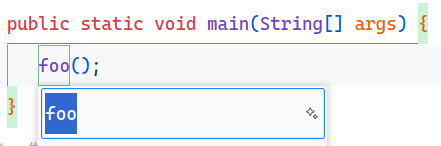
\includegraphics[width=4cm]{img/java-rename.png}};
            \node[below left] at(@.south east) {\scriptsize\textit{Rename Refactoring}};
         }
         \onslide<4-6|handout:1>{
            \node[draw,lightgray,inner sep=0pt,right=9.5mm] (@) at(@.east) {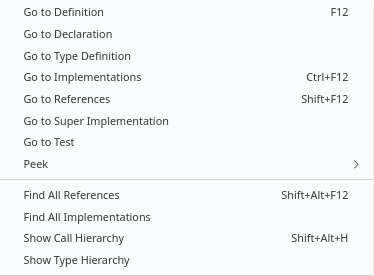
\includegraphics[width=4cm]{img/java-actions.png}};
            \node[below left] at(@.north west) {\scriptsize\textit{Code Actions}};
         }
         \onslide<5-6|handout:1>{%
            \node[right=4mm] at(current bounding box.east) {\ldots}; % types for typescript, ...
         }
      \end{tikzpicture}}\only<7-|handout:2>{~\\\color{gray}Renaming, Code Actions,~\ldots}
      \item<6-> Relies on the \link{https://github.com/eclipse/eclipse.jdt.ls}{Eclipse JDT Language Server}
   \end{itemize}
   
\begin{uncoverenv}<8-|handout:2>
\begin{tikzpicture}[o/.style={outer sep=0pt,inner sep=0pt},remember picture]
   \node[o] (@) at (0,0) {\usebox\CodeFile};
   \node[above=2.5mm,xshift=1.15mm,gray] at(@.north) {\textsb{\normalsize Input}};
\pgfonlayer{background}
\scope[transparency group,opacity=.4]
\node[o,rotate around={-30:(@.south east)},anchor=south east] at(@.south east) {\usebox\CodeFile};
\node[o,rotate around={-12:(@.south east)},anchor=south east] at(@.south east) {\usebox\CodeFile};
\endscope
\endpgfonlayer
\coordinate (@) at(@.east);
\foreach[count=\i] \usecase/\targeti in {{\raisebox{1pt}{Textual}}/0,Syntactical/0, Semantical/0, Historical/1, Annotated/0, {\raisebox{-3pt}{Metadata,~\ldots}}/0} { % program spectra, hardware, contexts, ...
\pgfmathsetmacro\rot{-24*\i+66}
      \path ([xshift=.5mm]@.east)++(\rot+10:1mm) coordinate (@a);
      \fill[opacity=.18,gray] (@a.east) -- ++(\rot:1.5cm) arc (\rot:\rot+20:1.5cm) -- cycle;
      \draw[thick,gray] (@a.east)++(\rot:1.5cm) arc (\rot:\rot+20:1.5cm);
      \tikzset{@/.style={}}
      \ifnum\targeti=1relax
         \only<9->{
            \tikzset{@/.style={opacity=.2}}
         }
      \fi
      \path (@a.east) -- ++(1.05*\rot+10:1.6cm) node[right,font=\small,darkgray,@] (@uc-\i) {\vphantom{a}\smash{\usecase}};
}
\coordinate (@east) at (current bounding box.east);
\onslide<10->{%
   \draw[decoration={brace},decorate,gray] ([yshift=.5mm]@uc-2.north east-|@uc-3.north east) -- ([yshift=-.5mm]@uc-3.south east) node[midway,right=1mm,font=\footnotesize,align=left] (jbc) {Mostly traverses\\the AST}; % using java byte code is rather common
}
\node[above=1.65mm,xshift=1mm,gray] at(current bounding box.north) {\textsb{\normalsize Perspectives}};
\begin{onlyenv}<-7|handout:0>
\node[right,yshift=-7mm,xshift=1cm,align=left,font=\small,darkgray,text width=3.25cm] (@techn) at(@east){{{{Text/Code Search}\strut}}~\\[4mm]\strut{{{Clustering}}}~\\[4mm]\strut{{{Abstract Domains}}}~\\[4mm]\strut{{{Dataflow Constraints}}}~\\[1mm]\strut{{\centerline{\footnotesize\(\vdots\)}}}};
\node[above=1.5mm,gray,xshift=-4.5mm] at(@techn.north) {\textsb{\normalsize Theory}};
\scope[gray,line cap=round]
   \draw ([yshift=1.5pt]@uc-1.east) -- ([yshift=-2.5mm]@techn.north west);
   \draw ([yshift=1.5pt]@uc-2.east) -- ([yshift=-2.5mm]@techn.north west);
   \draw[densely dotted] ([yshift=1.5pt]@uc-3.east) -- ([yshift=-2.5mm]@techn.north west);
   \draw ([yshift=1.5pt]@uc-1.east) -- ([yshift=-10.5mm]@techn.north west);
   \draw ([yshift=0pt]@uc-2.east) -- ([yshift=-10.5mm]@techn.north west);
   \draw ([yshift=1.5pt]@uc-4.east) -- ([yshift=-10.5mm]@techn.north west);
   
   \draw ([yshift=-1pt]@uc-2.east) -- ([yshift=-18.5mm]@techn.north west);
   \draw ([yshift=-1pt]@uc-3.east) -- ([yshift=-18.5mm]@techn.north west);
   \draw ([yshift=1.5pt]@uc-5.east) -- ([yshift=-18.5mm]@techn.north west);
   
   \draw ([yshift=-1pt]@uc-2.east) -- ([yshift=-26mm]@techn.north west);
   \draw ([yshift=-1pt]@uc-3.east) -- ([yshift=-26mm]@techn.north west);
\endscope
   
   \node[right=7.5mm] (@) at(current bounding box.east) {\resizebox*!{2.85cm}{\usebox\UiBox}};
   \scope[transparency group,opacity=.5,every path/.append style={line cap=round,line width=.5pt}]
      \draw[-Kite,gray] ([yshift=-2.5mm,xshift=-6.5mm]@techn.north east) to[out=0,in=180] ([xshift=1.5mm,yshift=-6.35mm]@.west);
      \draw[-Kite,gray] ([yshift=-10.5mm,xshift=-18.5mm]@techn.north east) to[out=0,in=180] ([xshift=7.15mm,yshift=-1.35mm]@.west);
      \draw[-Kite,gray] ([yshift=-18.5mm,xshift=-6.25mm]@techn.north east) to[out=0,in=180] ([xshift=26.15mm,yshift=-9.35mm]@.west);
      \draw[-Kite,gray] ([yshift=-26mm,xshift=-2.5mm]@techn.north east) to[out=0,in=180] ([xshift=26.15mm,yshift=-9.35mm]@.west);
   \endscope
   \node[above, gray] at(@.north) {\tiny \textsb{\normalsize Communicate} or \textsb{\normalsize Use}};
\end{onlyenv}
\onslide<11->{%
   \draw[gray,-Kite] (@uc-1.east) to[out=0,in=180] ++(6mm,2.5mm) node[right,font=\footnotesize,align=left] {Text Search,~\ldots};
}
\onslide<12->{%
   \draw[gray,-Kite] (@uc-5.east) to[out=0,in=180] ++(6.5mm,2mm) node[below right,font=\footnotesize,yshift=.7\baselineskip,align=left] {Annotation support,~\ldots};
}
\onslide<13->{%
   \draw[gray,-Kite] (@uc-6.east) to[out=0,in=180] ++(6.5mm,2mm) node[below right,font=\footnotesize,yshift=.7\baselineskip,align=left] {How to build the project,~\ldots};
}
\onslide<14->{
   \node[above=3.5mm,gray,xshift=17.5mm] (theory) at(@techn.north) {\textsb{\normalsize Theory}};
}
\onslide<15->{
   \node[below=1mm,align=right,align=center,font=\footnotesize] (a-domains) at(theory.south) {\small A lot of\ldots\\AST Traversal}; %
   \draw[gray,-Kite] (jbc.east) to[out=40,in=180] (a-domains.west);
}

\begin{uncoverenv}<16->
   \node[right=17.5mm,yshift=-.5mm,gray] (communicate) at(theory.east) {\textsb{\normalsize Communicate}};
   \node[below=1mm,thick,inner sep=0pt,align=center,font=\small] (jav-com) at(communicate.south) {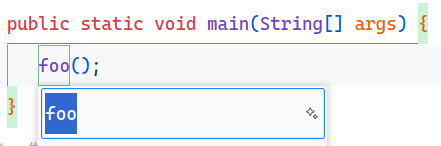
\includegraphics[width=3cm]{img/java-rename.png}};
   \draw[gray,-Kite] (a-domains.east) to[out=0,in=170] (jav-com.west);
\end{uncoverenv}
\end{tikzpicture}
\end{uncoverenv}
   
   \begin{tikzpicture}[overlay,remember picture]
      \node[below left=4mm] at(current page.north east) {\Logo[1cm]{https://github.com/redhat-developer/vscode-java}{redhat-vscode-java}};
      \node[above right,yshift=4mm,bottom note] at(current page.south west) {\link{https://github.com/eclipse-jdtls/eclipse.jdt.ls}{github.com/eclipse-jdtls/eclipse.jdt.ls}};
   \end{tikzpicture}
\end{frame}

\subsection{lintr}
\againframe<7,20|handout:6>{tool-slide}
\begin{frame}[fragile]{lintr}
\lstfs{8}
   \begin{itemize}
      \item<2-> A linter for the \tikzmarknode{r-prog-lang}{R programming language}
\begin{columns}[onlytextwidth,c]
\column{.04\linewidth}
\column{.3\linewidth}
\begin{onlyenv}<4-7|handout:0>
\begin{minted}[escapeinside=||]{R}
|\onslide<4->|x <- 4
|\onslide<5->|f <- function() x
|\onslide<6->|f() |\onslide<7->|# 4|\onslide<1->|
\end{minted}
\end{onlyenv}
\begin{onlyenv}<8-|handout:1>
\AnimateCode{onslide={o3:{4},-,-,-,-},first slide=8,handout=9/1}
\begin{minted}[escapeinside=||]{R}
|\onslide<8->|x <- 4
|\onslide<8->|f <- function() x
|\onslide<9->|body(f) <- quote(y)
|\onslide<9->|y <- 42
|\onslide<8->|f() |\onslide<10->|# |\textcolor{black}{\textbf{42}}||\onslide<1->|
\end{minted}
\endAnimateCode
\end{onlyenv}
\column<11-|handout:1>{.365\linewidth}
\color{black}\vspace*{-\baselineskip}%
\begin{minted}[escapeinside=||]{R}
|\onslide<12->|`if` <- function(...) 42|\onslide<1->|
if(TRUE) print(3) # |\xlstGetStyle{comments}\only<-11|handout:0>{3}\only<12-|handout:1>{42}||\onslide<1->|
\end{minted}
\column<13-|handout:1>{.3\linewidth}
\color{black}\vspace*{-\baselineskip}%
\begin{minted}[escapeinside=||]{R}
x <- 2
|\onslide<14->|`<-` <- `*`|\onslide<1->|
y <- 21 |\onslide<14->|# 42|\onslide<1->|
\end{minted}
\end{columns}\color{black}
\vspace*{-1\baselineskip}

   \item<15-|handout:1> \color{black}Common static analysis strategies have their\ldots{} problems with R
   \item<16-|handout:1> \color{black}Most of R's users are no computer scientists \onslide<17->{\color{gray}\footnotesize(just a small set of existing work)}
   \item<18-|handout:1> \color{black}So\ldots{} how does \textit{lintr} do it?
   \begin{itemize}
      \item<19-|handout:1> \only<20->{\expandafter\sout}{Dataflow Constraints?}
      \item<21-|handout:1> \only<22->{\expandafter\sout}{Abstract Domains?}
      \item<23-|handout:1> \only<24->{\expandafter\sout}{Control Flow Graphs?}
      \item<25-|handout:1> AST \only<26->{\expandafter\sout}{Traversal?} \only<27->{\textcolor{gray}{(mostly)} Pattern Matching and Evaluation!}
   \end{itemize}
\end{itemize}
\begin{tikzpicture}[overlay,remember picture]
   \node[below left=4mm] at(current page.north east) {\Logo[1.4cm]{https://github.com/r-lib/lintr}{lintr}};
   \node[above right,yshift=4mm,bottom note] at(current page.south west) {\link{https://github.com/r-lib/lintr}{github.com/r-lib/lintr}};
   \node[above left,yshift=4mm,bottom note] at(current page.south east) {\cite{DBLP:conf/dls/FluckigerCJYHV19}~\citetitle{DBLP:conf/dls/FluckigerCJYHV19} (\citeauthor{DBLP:conf/dls/FluckigerCJYHV19})}; 
   \onslide<3->{%
      \draw[Kite-,gray] ([xshift=2mm,yshift=.25mm]r-prog-lang.north west) to[out=70,in=180] ++(3mm,5mm) node[right,bottom note,yshift=-.15mm] {Why is this\ldots{} special?};
   }
\end{tikzpicture}
\end{frame}

\begin{frame}[fragile]{\textcolor{gray}{lintr ---~} Under the Hood}
\lstfs{8}\color{black}%
\onslide<4->{{\scriptsize\color{gray}\link{https://github.com/r-lib/lintr/blob/427fab3f2a82b824f3cdbfaf936228ed544f70a4/R/object_usage_linter.R\#L38}{\hbox{\faFileCodeO~}R/object\_usage\_linter.R}}}\vspace*{-.2\baselineskip}
\begin{minted}[prebreak={},escapeinside={|@}{@|},columns=fixed]{R}
|@\onslide<2->@|magic <- "
   expr[LEFT_ASSIGN or EQ_ASSIGN]/expr[2][FUNCTION or OP-LAMBDA]
   | expr_or_assign_or_help[EQ_ASSIGN]/expr[2][FUNCTION or OP-LAMBDA]
   | equal_assign[EQ_ASSIGN]/expr[2][FUNCTION or OP-LAMBDA]
   | //SYMBOL_FUNCTION_CALL[text() = 'assign']/parent::expr/following-sibling::expr[2][FUNCTION or OP-LAMBDA]
   | //SYMBOL_FUNCTION_CALL[text() = 'setMethod']/parent::expr/following-sibling::expr[3][FUNCTION or OP-LAMBDA]"|@\onslide<1->@|
\end{minted}
\vspace*{-.65\baselineskip}
\begin{itemize}
   \itemsep4pt
   \item<3-> What does this do?\\*
      \onslide<4->{This XPATH expression matches assignments to functions}
   \item<5-> It is very rigid (no alias tracking, flow sensitivity,~\ldots)
   \item<6-> And it\ldots{} \onslide<7->{cheats:}\vspace*{-.25\baselineskip}
\begin{uncoverenv}<8->
\begin{minted}[escapeinside={|@}{@|},morekeywords={[2]{eval,parse,try_silently}}]{R}
try_silently(eval(envir = env,parse(text = code, keep.sou:c:rce = TRUE)))
\end{minted}
\vspace*{-.33\baselineskip}
      \onslide<9->{It simply runs \textcolor{gray}{(parts of)} the program (including side-effects),~\ldots}
\end{uncoverenv}
\end{itemize}
\begin{tikzpicture}[overlay,remember picture]
   \node[below left=5mm] at(current page.north east) {\(\approx\)\;100 rules};
\end{tikzpicture}
\end{frame}

\color{black}
\subsection{flowR}
\let\T\texttt
\def\Content#1#2{#1\\[-.6ex]\smaller\textit{\color{gray}#2}}
\againframe<7,21|handout:7>{tool-slide}
\newsavebox\ShookPingu
\savebox\ShookPingu{\tikz{\pingu[wings shock,eyes shock,tie]}}
\def\y{&\G\faCircle} % yes
\def\planned{}% \llap{\smash{\raisebox{.95pt}{\faCaretUp}\kern1.33pt}}
\def\gy{&\color{gray}\G\faCircle} % yes but presented by dynamic analysis
% \def\m{&\G\faDotCircleO} % most but not all
\def\p{&\G\faCircleO} % partial | faDotCircleO ?
% probable (e.g. with eval)
\def\n{&\G\phantom{\faCircleO}}               % no
\protected\def\rhead#1{\makecell[b{l}]{\rlap{\sffamily\rotatebox{45}{\strut#1\strut}}}}

\def\G{\ifactive\else\color{lightgray!80!gray}\fi}

\pgfqkeys{/overview}{
   name/.code                = \xdef\oName{#1},
   cite/.code                = \gdef\oCite{#1},
   active/.code              = \xdef\oActive{#1},
   last updated/.code        = \gdef\oLastUpdated{#1},
   method/.code              = \gdef\oMethod{#1},
   goal/.code                = \gdef\oGoal{#1},
   doc url/.code             = \gdef\oDocUrl{#1},
   impl language/.code       = \gdef\oImplLanguage{#1},
   references/.code          = \gdef\oReferences{#1},
   assignments/.code         = \gdef\oAssignments{#1},
   func assignments/.code    = \gdef\oFunctionAssignments{#1}, % like s3,s4, assign...
   value tracing/.code       = \gdef\oValueTracing{#1},
   controlflow/.code         = \gdef\oControlflow{#1},
   non-standard eval/.code   = \gdef\oNonStandardEval{#1},
   (special) operators/.code = \gdef\oOperators{#1},
   function calls/.code      = \gdef\oFunctionCalls{#1},
   libraries/.code           = \gdef\oLibraries{#1},
   quotation/.code           = \gdef\oQuotation{#1},
   reflection/.code          = \gdef\oReflection{#1},
   side effects/.code        = \gdef\oSideEffects{#1},
   static scope/.code        = \gdef\oStaticScope{#1},
   dynamic scope/.code       = \gdef\oDynamicScope{#1}, % includes closures (which require side effects as well)!
   pointer analysis/.code    = \gdef\oPointerAnalysis{#1}, % tracks vectors, methods, ...
   external files/.code      = \gdef\oExternalFiles{#1},
   processors/.code          = \gdef\oProcessors{#1},
   hooks/.code               = \gdef\oHooks{#1},
   ffi/.code                 = \gdef\oFFI{#1},
   types/.code               = \gdef\oTypes{#1},%
   exposes df/.code           = \gdef\oExposesDf{#1},%
   @defaults/.style          = {
      references=\n,
      assignments=\n,func assignments=\n,value tracing=\n,controlflow=\n,non-standard eval=\n,
      (special) operators=\n,function calls=\n,libraries=\n,quotation=\n,
      reflection=\n,side effects=\n,static scope=\n,dynamic scope=\n,pointer analysis=\n,
      external files=\n,processors=\n,hooks=\n,ffi=\n,types=\n,doc url={},exposes df=\n%
   }
}
\newif\ifactive
\edef\activeyes{y}

\makeatletter
\def\Row#1{%
   \stepcounter{NumberOfToolRows}\pgfqkeys{/overview}{@defaults,#1}%
   \ifx\oActive\activeyes\global\activetrue\else\hypersetup{allcolors=.}\global\activefalse\fi
   {\def\{{xy}\def\}{yx}\def\v{vv}\xdef\tname{\oName}}%
   \tikzmarknode{\tname @start}\strut
   \G\kern1.5em\llap{\ifx\oCite\empty\else\edef\tmp{\noexpand\cite{\oCite}}\tmp\fi}&
   %& \G\oLastUpdated
   \G{\hypersetup{allcolors=.}\href{\oDocUrl}{\texttt{\oName}}}
   % & \G\oImplLanguage %
   \oReferences
   \oAssignments
   \oFunctionAssignments
   \oValueTracing
   \oControlflow
   \oNonStandardEval
   \oOperators
   \oFunctionCalls
   \oLibraries
   \oReflection
   \oSideEffects
   \oStaticScope
   \oDynamicScope
   \oTypes
   \oPointerAnalysis
   \oExternalFiles
   \oProcessors
   \oHooks
   \oFFI 
   \oExposesDf
   & 
   \G\oGoal & \G\oMethod 
   \tikzmarknode{\tname @end}\strut
   % \ifactive\else
   %    \tikz[overlay,remember picture]{\draw[line cap=round,lightgray,opacity=.8]([xshift=-1mm,yshift=1pt]\tname @start.east)coordinate (@)--([xshift=1mm]@-|\tname @end.east);}%
   % \fi
}

\newcounter{headercount}
\def\headcount#1{%
\rhead{#1}% ~\stepcounter{headercount}(\theheadercount)
}


\def\TableHeader{& & % impl. lang. &
\headcount{references} &
\headcount{op. assignments} & \headcount{dyn. assignments} &  \headcount{value trace} & \headcount{control flow} & \headcount{non-std. eval.} & \headcount{special operators} & \headcount{function calls} & \headcount{libraries} & \headcount{reflection} & \headcount{side effects} & \headcount{static scope} & \headcount{dynamic scope} & \headcount{type inference} & \headcount{pointer analysis} & \headcount{external files} & \headcount{pre-processors} & \headcount{hooks} & \headcount{FFI} & \headcount{expose info.} & \textsf{goal} & \textsf{method}}

\begin{frame}{Existing Work}
\vspace*{-3\baselineskip}\centering
\begin{onlyenv}<2->
   \color{black}
   \def\skp{\hskip7pt}
   % Reaching definitions, Liveness analysis, Definite assignment analysis, Available expression, Constant propagation
   % ===================================================================
   % help from:
   % https://indrajeetpatil.github.io/awesome-r-pkgtools
   % nothing from: https://github.com/qinwf/awesome-R
   % ===================================================================
   \resizebox*{.75\linewidth}{!}{\begin{tabular}{>{\color{lightgray}}r@{\hskip3pt}l*{4}{*{5}{@{\hskip6pt}c}}>{\sffamily\kern3mm}l@{\skp}>{\sffamily}l}
      \TableHeader\\
      \vphantom{\huge I}\only<4->{\bfseries}
      % it is us!
\Row{
   name                = flowR,
   doc url             = {}, % https://github.com/Code-Inspect/flowr
   cite                = {}, % flowr_sihler_24
   active              = y,
   last updated        = 2024,
   method              = {AST visitor}, % & cfg
   goal                = {static analysis},
   impl language       = {TS, R},
%  -----------------------------------------------
   references          = \y, % we handle them
   assignments         = \y, % special assignment handler
   func assignments    = \p\planned, % only reduced support, we can not handle functions calling them indirectly (i.e., with value tracing)
   value tracing       = \p\planned, % currently work in progress, value tracing reduced by pointer tracks
   controlflow         = \y, % have separate cfg
   non-standard eval   = \p, % only some precautions but no real handling of all kinds of evaluation histories
   (special) operators = \y, % we handle them specifically
   function calls      = \y, % track including side effects and higher order functions
   libraries           = \p\planned, % we at least detect their load as a side effet
   quotation           = \p\planned, % some precautions (ignore)
   reflection          = \p, % neither body, nor substitute, ... but we break edges and mark unknown side effects!
   side effects        = \p, % we have side effects with <<- but not with env/pointers
   static scope        = \y, % yes, we \llap{\smash{\raisebox{.95pt}{\faCaretUp}\kern1.33pt}}have lexical scoping
   dynamic scope       = \p, % we try to track higher call hierarchies but we can not handle all
   pointer analysis    = \n\planned, % planned
   external files      = \p\planned, % sourcing but that is it atm more is planned
   processors          = \n, % no handling for the time
   hooks               = \n, % no handling for the time
   ffi                 = \n, % no handling for the time
   types               = \n, % no handling for the time
   exposes df          = \y, % this is our whole thing :D
}\\%
      % non-colored pad
      \strut \\[\dimexpr-.8\ht\strutbox]
      % fragen:
% 1. einzelne doch ausblenden
% 2. dynamische noch einblenden?
% 3. wie strikt sein wenn base::eval genutzt wird für abstract interpretation?
% 4. zweite Person drüberschauen lassen?
% 5. Wie sind die Kategorien?
% https://memtools.r-lib.org/
% only a few of them are just built for static analysis, funnily not all
% of course just not having something does not mean that they _need_ it

% has a large list of predefined function names (https://github.com/JorisChau/checkglobals/blob/master/src/utils.c)
\Row{
   name                = \{checkglobals\},
   doc url             = {https://cran.r-project.org/package=checkglobals},
   cite                = {checkglobals_chau_23},
   active              = y,
   last updated        = 2023,
   method              = AST visitor,
   goal                = missing libs., % and function defs
   impl language       = {R, C},
%  -----------------------------------------------
   references          = \y, % i mean, they track global references
   assignments         = \y, % special assignment handler
   func assignments    = \p, % handles them as simple local assigns
   value tracing       = \n, % handles no values
   controlflow         = \n, % just traverses all branches; only for loop? not repeat/while
   non-standard eval   = \p, % have special function handlers for eval
   (special) operators = \p, % treated as calls
   function calls      = \p, % i mean, it has a very reduced list of functions it deals with
   libraries           = \p, % imports their exported namespace/what is loaded with :: and :::
   quotation           = \p, % just ignores the content
   reflection          = \n, % neither body, nor substitute, ...
   side effects        = \n, % does not handle fcalls to my knowledge
   static scope        = \p, % just has global/not global
   dynamic scope       = \n, % no, no eval.parent etc?
   pointer analysis    = \n, % no handling
   external files      = \n, % i mean they detect them, but no load (if not R package and R support)
   processors          = \n, % i can find no support whatsoever
   hooks               = \n, % does not appear
   ffi                 = \p, % tracks .C, .External, ...
   types               = \n % no type information
   }\\%
% uses rstatic, CodeDepends
\Row{
   name                = \{CodeAnalysis\},
   doc url             = {https://github.com/duncantl/CodeAnalysis},
   cite                = {lang_codeanalysis_2023},
   active              = y,
   last updated        = 2023,
   method              = AST visitor, % + normalization of rstatic
   goal                = static analysis,
   impl language       = R,
%  -----------------------------------------------
   references          = \y, % identifies where they are defined
   assignments         = \y, % special assignment handler
   func assignments    = \p, % have a process expr which at least recognizes them
   value tracing       = \p, % trace back if variables have a constant value, no propagation
   controlflow         = \y, % given by codetools code walker and rstatic with the cfg
   non-standard eval   = \p, % has code depends handlers
   (special) operators = \p, % treated as calls
   function calls      = \p, % just link calls but do not traverse for side-effects (but have the wish for it); have a callgraph/traverse given closures
   libraries           = \p, % rely on Code Depends
   quotation           = \p, % just ignores the content
   reflection          = \n, % neither body, nor substitute, ...
   side effects        = \n, % not supported; to my knowledge they ignore code depends here
   static scope        = \y, % yes, have lexical scoping
   dynamic scope       = \n, % no, no eval.parent etc?
   pointer analysis    = \n, % they just track values
   external files      = \p, % track sourced files
   processors          = \n, % i can find no support whatsoever
   hooks               = \n, % does not appear
   ffi                 = \n, % does not appear
   types               = \p,  % it re-exposes the table view of RTypeInference
   exposes df          = \y
}\\%
\Row{%
   name                = \{CodeDepends\},
   doc url             = {https://cran.r-project.org/package=CodeDepends},
   cite                = lang_codedepends_2018,
   active              = y,
   last updated        = 2023,
   method              = AST visitor,
   goal                = static analysis,
   impl language       = R,
%  -----------------------------------------------
   references          = \y, % identifies where they are defined
   assignments         = \y, % special assignment handler; should support limited set of
   func assignments    = \p, % handles *only* assign
   value tracing       = \n, % handles no values
   controlflow         = \n, % just traverses all branches; only for loop? not repeat/while
   non-standard eval   = \p, % have special function handlers for eval
   (special) operators = \p, % treated as calls
   function calls      = \p, % they traverse them but does not link with redefs?
   libraries           = \p, % use their export list
   quotation           = \n, % has to my knowledge no handling for it
   reflection          = \n, % neither body, nor substitute, ...
   side effects        = \p, % has a fixed list of side effects it recognizes
   static scope        = \y, % yes, have lexical scoping
   dynamic scope       = \n, % no, no eval.parent etc?
   pointer analysis    = \n, % they just track values
   external files      = \n, % i mean they detect them, but no load (if not R package and R support)
   processors          = \n, % i can find no support whatsoever
   hooks               = \n, % does not appear
   ffi                 = \n, % does not appear
   types               = \n, % nothing
   exposes df          = \y
}\\%

% https://gitlab.com/luke-tierney/codetools/-/blob/master/R/codetools.R?ref_type=heads
\Row{
   name                = \{codetools\},
   doc url             = {https://cran.r-project.org/package=codetools},
   cite                = {codetools_tierney_23},
   active              = y,
   last updated        = 2023,
   method              = AST visitor,
   goal                = static analysis, % has checkUsage which finds some problems
   impl language       = R,
%  -----------------------------------------------
   references          = \y, % identifies where they are defined
   assignments         = \y, % special assignment handler
   func assignments    = \p, % only assign and delayed assign
   value tracing       = \p, % limited constant folding and abstract interpretation for function (eval)
   controlflow         = \p, % uses abstract interpretation to check with current env but no return, continue, break
   non-standard eval   = \p, % have special function handlers for eval
   (special) operators = \p, % treated as calls
   function calls      = \p, % they traverse definitions but not resolved/just checks usage
   libraries           = \n, % does not include libraries
   quotation           = \p, % simply ignores content
   reflection          = \n, % neither body, nor substitute, ...
   side effects        = \n, % does not handle fcalls to my knowledge
   static scope        = \y, % yes, have lexical scoping
   dynamic scope       = \n, % no, no eval.parent etc?
   pointer analysis    = \n, % they just track values
   external files      = \n, % nothing for source etc!
   processors          = \n, % i can find no support whatsoever
   hooks               = \n, % does not appear
   ffi                 = \n, % does not appear
   types               = \n, % no type information
   exposes df          = \y
}\\%

\Row{
   name                = \{cyclocomp\},
   doc url             = {https://cran.r-project.org/package=cyclocomp},
   cite                = {cyclocomp_csardi_23},
   active              = y,
   last updated        = 2023,
   method              = AST visitor, % usually walker
   goal                = static analysis,
   impl language       = R,
%  -----------------------------------------------
   references          = \n, % identifies where they are defined
   assignments         = \n, % no handling
   func assignments    = \n, % no handling
   value tracing       = \n, % handles no values
   controlflow         = \p, % tracks them for the complexity
   non-standard eval   = \n, % no handling
   (special) operators = \n, % no handling
   function calls      = \n, % i mean it handles for etc. as calls but we do not score this for the others
   libraries           = \n, % no handling
   quotation           = \n, % no handling
   reflection          = \n, % neither body, nor substitute, ...
   side effects        = \n, % does not handle fcalls to my knowledge
   static scope        = \y, % yes, they have a stack for the function ids
   dynamic scope       = \n, % no, no eval.parent etc?
   pointer analysis    = \n, % no
   external files      = \n, % no
   processors          = \n, % no handling
   hooks               = \n, % no handling
   ffi                 = \n, % no handling
   types               = \n  % no type information
}\\%
\Row{
   name                = \{DependenciesGraphs\},
   doc url             = {https://github.com/datastorm-open/DependenciesGraphs},
   cite                = {dependenciesgraphs_robert_16},
   active              = n,
   last updated        = 2016,
   method              = regex,
   goal                = {visualize}, % dependencies
   impl language       = {R},
%  -----------------------------------------------
   references          = \n, % no handling
   % this uses mvbutils and some additional handling for libraries
   assignments         = \n, % no handling
   func assignments    = \n, % no handling
   value tracing       = \n, % no handling
   controlflow         = \n, % no handling
   non-standard eval   = \n, % no handling
   (special) operators = \n, % no handling
   function calls      = \p, % with foodweb
   libraries           = \p, % recognizes some limited loads with regexp?
   quotation           = \n, % no handling
   reflection          = \n, % no handling
   side effects        = \n, % no handling
   static scope        = \n, % no handling
   dynamic scope       = \n, % no handling
   pointer analysis    = \n, % no handling
   external files      = \n, % no handling
   processors          = \n, % no handling
   hooks               = \n, % no handling
   ffi                 = \n, % no handling
   types               = \n, % no handling
   exposes df          = \p
}\\%
% https://github.com/dkary/dfgraph/blob/main/ref/POC.md
\Row{
   name                = \{dfgraph\},
   doc url             = {https://github.com/dkary/dfgraph},
   cite                = {dfgraph_kary_23},
   active              = n,
   last updated        = 2021,
   method              = AST visitor,
   goal                = static analysis,
   impl language       = R,
%  -----------------------------------------------
   references          = \y, % handles based on what is known to be defined 
   assignments         = \p, % '<-', '='
   func assignments    = \n, % no
   value tracing       = \n, % no
   controlflow         = \p, % if
   non-standard eval   = \n, % no
   (special) operators = \n, % no
   function calls      = \p, % i mean it makes a call graph :eyes:
   libraries           = \n, % no
   quotation           = \n, % no
   reflection          = \n, % no
   side effects        = \n, % no
   static scope        = \n, % no
   dynamic scope       = \n, % no
   pointer analysis    = \n, % no
   external files      = \n, % no
   processors          = \n, % no
   hooks               = \n, % no
   ffi                 = \n, % no
   types               = \n,  % no type information
   exposes df          = \p
}\\%
% relatively young
% nice graphic outputs
% TODO: rpp and typed?
\Row{
   name                = \{flow\},
   doc url             = {https://cran.r-project.org/package=flow},
   cite                = {flow_fabri_23},
   active              = y,
   last updated        = 2023,
   method              = AST visitor,
   goal                = {vis., debug},% ualize
   impl language       = {R, C},
%  -----------------------------------------------
   references          = \y, % [TODO] check with sources resolve against
   assignments         = \p, % only <-, -> ... and = but not, e.g. ->> as far as i can see
   func assignments    = \n, % not supported
   value tracing       = \n, % just deparsed but not resolved
   controlflow         = \y, % visualizes them with separate condition and handles basic blocks
   non-standard eval   = \n, % to my knowledge not handled?
   (special) operators = \p, % treated as calls as far as i can see, part of the special handlings
   function calls      = \n, % to my knowledge they are just part of the basic blocks
   libraries           = \p, % reads the DESCRIPTION file of a package are just ignored
   quotation           = \p, % limited handling for quote ~ and function but not substitute and the like
   reflection          = \n, % neither body, nor substitute, ...
   side effects        = \n, % no calls
   static scope        = \n, % do not seem to handle function definitions at all
   dynamic scope       = \n, % no, no eval.parent etc?
   pointer analysis    = \n, % far from it
   external files      = \p, % visualizes sources
   processors          = \n, % i can find no support whatsoever
   hooks               = \n, % does not appear
   ffi                 = \n, % does not appear
   types               = \n, % no type information
   exposes df          = \p
}\\%
% pointed out to me by hadley wickham
\Row{
   name                = \{foodwebr\},
   doc url             = {https://github.com/lewinfox/foodwebr},
   cite                = {foodwebr_appleton-fox_24},
   active              = y,
   last updated        = 2023,
   method              = regex, % name matching,
   goal                = {visualize},
   impl language       = {R},
%  -----------------------------------------------
   % this one is tricky as even though it does not do any real analysis itself (regarding assignments etc.)
   % it requires and environment to do the trick.
   references          = \n, % no handling
   assignments         = \n, % no handling
   func assignments    = \n, % no handling
   value tracing       = \n, % no handling
   controlflow         = \n, % no handling
   non-standard eval   = \n, % no handling
   (special) operators = \n, % no handling
   function calls      = \p, % tries to resolve them to the environment
   libraries           = \n, % no handling
   quotation           = \n, % no handling
   reflection          = \n, % no handling
   side effects        = \n, % no handling
   static scope        = \n, % no handling
   dynamic scope       = \n, % no handling
   pointer analysis    = \n, % no handling
   external files      = \n, % no handling
   processors          = \n, % no handling
   hooks               = \n, % no handling
   ffi                 = \n, % no handling
   types               = \n,  % no handling
   exposes df          = \p
}\\%
% uses codetools
\Row{
   name                = \{globals\},
   doc url             = {https://cran.r-project.org/package=globals},
   cite                = {globals_bengtsson_22},
   active              = y,
   last updated        = 2023,
   method              = AST visitor,
   goal                = distributed env., % / parallel, ...
   impl language       = R,
%  -----------------------------------------------
   % essentially just what codetools is capable of
   references          = \y, % similar to code tools
   assignments         = \y, % special assignment handler
   func assignments    = \n, % can not find any handling
   value tracing       = \p, % limited constant folding and abstract interpretation for function
   controlflow         = \p, % uses abstract interpretation to check with current env but no return, continue, break
   non-standard eval   = \p, % have special function handlers for eval
   (special) operators = \p, % treated as calls
   function calls      = \p, % they traverse definitions but not resolved/just checks usage
   libraries           = \n, % does not include libraries
   quotation           = \p, % simply ignores content
   reflection          = \n, % neither body, nor substitute, ...
   side effects        = \n, % does not handle fcalls to my knowledge
   static scope        = \y, % yes, have lexical scoping
   dynamic scope       = \n, % no, no eval.parent etc?
   pointer analysis    = \n, % they just track values
   external files      = \n, % nothing for source etc!
   processors          = \n, % i can find no support whatsoever
   hooks               = \n, % does not appear
   ffi                 = \n, % does not appear
   types               = \n  % no type information
}\\%
\Row{
   name                = \{languageserver\},
   doc url             = {https://cran.r-project.org/package=languageserver},
   cite                = {languageserver_lai_23},
   active              = y,
   last updated        = 2024,
   method              = {XPath, visitor},
   goal                = editor support,
   impl language       = {R, C},
%  -----------------------------------------------
   references          = \y, % they resolve against tracked named symbols
   assignments         = \y, % i mean they handle LEFT_/RIGHT_/EQ_ASSIGN
   func assignments    = \p, % they load them and directly execute a fixed list?
   value tracing       = \n, % handles no values
   controlflow         = \n, % does not consider (just during parsing to add to nonfuncs)
   non-standard eval   = \n, % no support
   (special) operators = \n, % no special handling
   function calls      = \p, % they do not link them always correctly but they resole them to whatever definition they find
   libraries           = \p, % load their exports and integrate them
   quotation           = \n, % nothing
   reflection          = \n, % neither body, nor substitute, ...
   side effects        = \n, % does not handle fcalls to my knowledge
   static scope        = \y, % yes, have lexical scoping
   dynamic scope       = \n, % no, no eval.parent etc?
   pointer analysis    = \n, %
   external files      = \n, % dont load?
   processors          = \n, % i can find no support whatsoever
   hooks               = \n, % does not appear
   ffi                 = \n, % does not appear
   types               = \n, % no type information
   exposes df          = \p
}\\%
% some lintr rules are much more sophisticated
\Row{
   name                = \{lintr\},
   doc url             = {https://cran.r-project.org/package=lintr},
   cite                = {lintr_hester_23},
   active              = y,
   last updated        = 2023,
   method              = {XPath, visitor}, % (AST visitor)
   goal                = linting,
   impl language       = R,
%  -----------------------------------------------
   references          = \y, % they have linters which do and linters which do not
   assignments         = \y, % special assignment handler
   func assignments    = \p, % only assign and set method in _one_ linter rule
   value tracing       = \n, % handles no values (besides constant placements etc. but not in a dataflow way)
   controlflow         = \p, % xpath dead code detection
   non-standard eval   = \n, % not used
   (special) operators = \p, % treated as calls
   function calls      = \n, % currently no one is tracing calls to my knowledge
   libraries           = \p, % unused library etc.
   quotation           = \n, % not used
   reflection          = \n, % neither body, nor substitute, ...
   side effects        = \n, % does not handle fcalls to my knowledge
   static scope        = \y, % yes, have lexical scoping
   dynamic scope       = \n, % no, no eval.parent etc?
   pointer analysis    = \n, % no rule deals with indirection as far as i can find
   external files      = \n, % i mean they detect them, but no load (if not R package and R support)
   processors          = \n, % i can find no support whatsoever
   hooks               = \n, % does not appear
   ffi                 = \n, % does not appear
   types               = \n % no type information
}\\%
\Row{
   name                = \{mvbutils\},
   doc url             = {https://CRAN.R-project.org/package=mvbutils},
   cite                = {mvbutils_bravington_18},
   active              = y,
   last updated        = 2018,
   method              = regex, % name matching,
   goal                = {utility},
   impl language       = {R},
%  -----------------------------------------------
   % i classify this like foodwebr... and only the foodweb function
   references          = \n, % no handling
   assignments         = \n, % no handling
   func assignments    = \n, % no handling
   value tracing       = \n, % no handling
   controlflow         = \n, % no handling
   non-standard eval   = \n, % no handling
   (special) operators = \n, % no handling
   function calls      = \p, % tries to resolve them to the environment
   libraries           = \n, % no handling
   quotation           = \n, % no handling
   reflection          = \n, % no handling
   side effects        = \n, % no handling
   static scope        = \n, % no handling
   dynamic scope       = \n, % no handling
   pointer analysis    = \n, % no handling
   external files      = \n, % no handling
   processors          = \n, % no handling
   hooks               = \n, % no handling
   ffi                 = \n, % no handling
   types               = \n  % no handling
}\\%
\Row{
   name                = \{PaRe\}, % + , \{typed\} % no longer on cran issues were not corrected in time
   doc url             = {https://cran.r-project.org/package=PaRe},
   cite                = {pare_van_kessel_23},
   active              = n,
   last updated        = 2023,
   method              = regex,
   goal                = code review,
   impl language       = R,
%  -----------------------------------------------
   references          = \n, % i cant find anything related to that
   assignments         = \p, % it can do <- for functions
   func assignments    = \n, % no (regex)
   value tracing       = \n, % no
   controlflow         = \p, % does not look at it personally, but uses cyclocomp for it
   non-standard eval   = \n, % no
   (special) operators = \n, % no
   function calls      = \p, % at least for the function( ... ) match :eyes:
   libraries           = \n, % no
   quotation           = \n, % no
   reflection          = \n, % no
   side effects        = \n, % no
   static scope        = \n, % no
   dynamic scope       = \n, % no
   pointer analysis    = \n, % no
   external files      = \n, % no
   processors          = \n, % no
   hooks               = \n, % no
   ffi                 = \n, % no
   types               = \n  % no
}\\%
% currently not on CRAN for (policy violation?)
% https://github.com/universal-ctags/ctags/blob/master/parsers/r.c
\Row{
   name                = \{pkgstats\},
   doc url             = {https://cran.r-project.org/package=pkgstats},
   cite                = {pkgstats_padgham_21},
   active              = y, % still developed
   last updated        = 2023,
   method              = {\href{https://ctags.io}{ctags} \& \href{https://www.gnu.org/software/global/}{gtags}},
   goal                = pkg. insights,
   impl language       = {R, C++},
%  -----------------------------------------------
   references          = \y, % i think they link on what is exported
   assignments         = \p, % it is relying on the symbols extracted by ctags/gtags
   func assignments    = \n, % to my knowledge ctags and gtags do not have support
   value tracing       = \n, % handles no values
   controlflow         = \n, % no support
   non-standard eval   = \n, % no support
   (special) operators = \p, % ctags recognizes them as values
   function calls      = \p, % not their effects, but they resolve their targets
   libraries           = \n, % i can not find them being of use
   quotation           = \n, % no support
   reflection          = \n, % no support
   side effects        = \n, % ctags/gtags does not track them
   static scope        = \p, % to my knowledge it is not as good in tracking them
   dynamic scope       = \n, % no support
   pointer analysis    = \n, % far from it
   external files      = \n, % not loaded etc.
   processors          = \n, % does not appear
   hooks               = \n, % does not appear
   ffi                 = \n, % does not appear
   types               = \n  % nothing
}\\%
% relies on code depends; essentially to a limited kind of program slicing on the existing pdg
\Row{
   name                = \{Rclean\},
   doc url             = {https://github.com/ropensci-archive/Rclean},
   cite                = {rclean_lau_22},
   active              = n,
   last updated        = 2022,
   method              = PDG traversal,
   goal                = debug/refactor,
   impl language       = R,
%  -----------------------------------------------
   % similar to code depends, adds nothing [but side effects!]
   references          = \y, % from code depends
   assignments         = \y, % from code depends
   func assignments    = \p, % from code depends
   value tracing       = \n, % from code depends
   controlflow         = \n, % from code depends
   non-standard eval   = \p, % from code depends
   (special) operators = \p, % from code depends
   function calls      = \p, % from code depends
   libraries           = \p, % from code depends
   quotation           = \n, % from code depends
   reflection          = \n, % from code depends
   side effects        = \n, % to my knowledge: just ignores them
   static scope        = \y, % from code depends
   dynamic scope       = \n, % from code depends
   pointer analysis    = \n, % from code depends
   external files      = \n, % from code depends
   processors          = \n, % from code depends
   hooks               = \n, % from code depends
   ffi                 = \n, % from code depends
   types               = \n  % no type inference
}\\%
% https://cran.r-project.org/web/packages/rco/vignettes/contributing-an-optimizer.html
% common subexpression
% cond thread (if-else resolve)
% constant folding and constant propagation
% dead-code elimination (store, expr)
% loop invariant hoisting
\Row{
   name                = \{rco\},
   doc url             = {https://cran.r-project.org/package=rco},
   cite                = {rco_rodriguez_21},
   active              = y, % appears to be n
   last updated        = 2021,
   method              = AST visitor, % recursive custom descent in a way but still
   goal                = optimization,
   impl language       = R,
%  -----------------------------------------------
   references          = \y, % referenced against names (e.g. for constant folds)
   assignments         = \y, % only operators no support for assignment functions! all in all very limited
   func assignments    = \n, % no handling
   % keywords            = \p, % only for
   % built ins           = \n, % no assign, etc
   value tracing       = \y, % constant folding and propagation
   controlflow         = \p, % supports condition threading/otherwise only for dead code
   non-standard eval   = \n, % not implemented
   (special) operators = \n, % treated as calls
   function calls      = \n, % planned but to my knowledge not implemented
   libraries           = \n, % not implemented
   quotation           = \n, % not implemented
   reflection          = \n, % neither body, nor substitute, ...
   side effects        = \n, % not implemented
   static scope        = \y, % track function envs
   dynamic scope       = \n, % no, no eval.parent etc?
   pointer analysis    = \n, % no
   external files      = \n, % i mean they detect them, but no load (if not R package and R support)
   processors          = \n, % i can find no support whatsoever
   hooks               = \n, % does not appear
   ffi                 = \n  % does not appear
}\\%

\Row{
   name                = {\{rflowgraph\}},
   doc url             = {https://github.com/IBM/rflowgraph},
   cite                = {flowgraph_patterson_19},
   active              = n,
   last updated        = 2019,
   method              = AST visitor,
   goal                = call graph,
   impl language       = R,
%  -----------------------------------------------
   references          = \y, % i mean, technically by function calls 
   assignments         = \n, % no
   func assignments    = \n, % no
   value tracing       = \n, % no
   controlflow         = \n, % no
   non-standard eval   = \n, % no
   (special) operators = \n, % no
   function calls      = \p, % has a call graph
   libraries           = \p, % i think, if given, they are included?
   quotation           = \n, % no
   reflection          = \n, % no
   side effects        = \n, % no
   static scope        = \n, % no
   dynamic scope       = \n, % no
   pointer analysis    = \n, % no
   external files      = \n, % no
   processors          = \n, % no
   hooks               = \n, % no
   ffi                 = \n, % no
   types               = \n, % no type information
   exposes df          = \p
}\\%
% can not handle replacement functions faik
\Row{
   name                = \{rstatic\},
   doc url             = {https://github.com/nick-ulle/rstatic},
   cite                = {rstatic_ulle_19},
   active              = n,
   last updated        = 2019,
   method              = AST visitor,
   goal                = static analysis,
   impl language       = R,
%  -----------------------------------------------
   references          = \y, % resolve in global scope
   assignments         = \y, % special assignment handler
   func assignments    = \n, % i can not find any handling
   value tracing       = \p, % constant propagation of simple values
   controlflow         = \y, % holds control flow graph (explicit and implicit returns, ...)
   non-standard eval   = \n, % have special function handlers for eval
   (special) operators = \p, % treated as calls
   function calls      = \n, % not tracked at all
   libraries           = \n, % are not handled
   quotation           = \n, % has to my knowledge no handling for it
   reflection          = \n, % neither body, nor substitute, ...
   side effects        = \n, % does not handle fcalls to my knowledge
   static scope        = \y, % yes, have lexical scoping
   dynamic scope       = \n, % no, no eval.parent etc?
   pointer analysis    = \n, % just stubbed
   external files      = \n, % i mean they detect them, but no load (if not R package and R support)
   processors          = \n, % i can find no support whatsoever
   hooks               = \n, % does not appear
   ffi                 = \n, % does not appear (just marked as todo)
   types               = \n, % handled by RTypeInferenc
   exposes df          = \y
}\\%
% can not handle replacement functions afaik
\Row{
   name                = \{RTypeInference\},
   doc url             = {https://github.com/duncantl/RTypeInference},
   cite                = {rtypeinference_ulle_21},
   active              = n,
   last updated        = 2021,
   method              = AST visitor,
   goal                = type inference,
   impl language       = R,
%  -----------------------------------------------
   references          = \y, % from rstatic
   assignments         = \y, % from rstatic
   func assignments    = \n, % from rstatic
   value tracing       = \p, % from rstatic
   controlflow         = \y, % from rstatic
   non-standard eval   = \n, % from rstatic
   (special) operators = \p, % from rstatic
   function calls      = \n, % from rstatic
   libraries           = \n, % from rstatic
   quotation           = \n, % from rstatic
   reflection          = \n, % from rstatic
   side effects        = \n, % from rstatic
   static scope        = \y, % from rstatic
   dynamic scope       = \n, % from rstatic
   pointer analysis    = \n, % from rstatic
   external files      = \n, % from rstatic
   processors          = \n, % from rstatic
   hooks               = \n, % from rstatic
   ffi                 = \n, % from rstatic
   types               = \y, % i mean it is limited by rstatic but it is there
   exposes df          = \p
}\\%
% there are others, dupree uses string similarity after token normalisation, rscc calculates similarity tables
\Row{
   name                = \{SimilaR\},
   doc url             = {https://cran.r-project.org/package=SimilaR},
   cite                = {similar_bartoszuk_23},
   active              = n, % n? Mails to maintainer is undeliverable
   last updated        = 2020,
   method              = {PDG, visitor}, % and similarity
   goal                = plagiarism,
   impl language       = {R, C++},
%  -----------------------------------------------
   references          = \y, % they at least track named symbols
   assignments         = \p, % only <- and =
   func assignments    = \n, % has only support for <- and =
   value tracing       = \n, % handles no values
   controlflow         = \p, % includes control flow edges but they appear to be partial
   non-standard eval   = \n, % have special function handlers for eval
   (special) operators = \n, % only has a very limited operator set
   function calls      = \p, % only limited set of built-ins
   libraries           = \n, % no support
   quotation           = \n, % no support
   reflection          = \n, % neither body, nor substitute, ...
   side effects        = \n, % does not handle fcalls to my knowledge
   static scope        = \y, % yes, creates sub CDGs
   dynamic scope       = \n, % no support
   pointer analysis    = \n, % no support
   external files      = \n, % no support
   processors          = \n, % no support
   hooks               = \n, % no support
   ffi                 = \n, % no support
   types               = \n  % no type information
}\\%
% \Row{
   name                = \{covr\},
   doc url             = {https://cran.r-project.org/package=covr},
   cite                = {covr_hester_23},
   active              = y,
   last updated        = 2023,
   method              = instrument,
   goal                = dynamic analysis,
   impl language       = {R, C},
%  -----------------------------------------------
   references          = \gy, % handled by dynamic execution
   assignments         = \gy, % handled by dynamic execution \p, % it ignores <- and = (`{`, ...)
   func assignments    = \gy, % handled by dynamic execution
   value tracing       = \gy, % handled by dynamic execution
   controlflow         = \gy, % handled by dynamic execution
   non-standard eval   = \gy, % handled by dynamic execution
   (special) operators = \gy, % handled by dynamic execution
   function calls      = \gy, % handled by dynamic execution
   libraries           = \gy, % handled by dynamic execution
   quotation           = \gy, % handled by dynamic execution
   reflection          = \gy, % handled by dynamic execution
   side effects        = \gy, % handled by dynamic execution
   static scope        = \gy, % yes, have lexical scoping
   dynamic scope       = \gy, % handled by dynamic execution
   pointer analysis    = \gy, % handled by dynamic execution
   external files      = \gy, % handled by dynamic execution
   processors          = \gy, % handled by dynamic execution
   hooks               = \gy, % handled by dynamic execution
   ffi                 = \p  % it has support for compiled functions (gcov)
}\\% % dynamic
% % has tidy eval etc. to make it more readable
\Row{
   name                = \{formatR\},
   doc url             = {https://cran.r-project.org/package=formatR},
   cite                = {formatR_xie_23},
   active              = y,
   last updated        = 2023,
   method              = walk-transform,
   goal                = pretty-print,
   impl language       = R
}\\%
% % similar to lintr, to automatically grade R scripts (no real sa)
\Row{
   name                = \{roger\}
   doc url             = {https://cran.r-project.org/package=roger},
   cite                = {roger_goulet_23},
   active              = y,
   last updated        = 2023,
   method              = {AST visitor}, %
   goal                = linting,
   impl language       = R,
%  -----------------------------------------------
   % essentially way less sophisticated
}\\% % is just lintr but waaaay less sophisitated and with much less tatic aalysis
% 
\Row{
   name                = \{styler\},
   doc url             = {https://cran.r-project.org/package=styler},
   cite                = {styler_muller_23},
   active              = y,
   last updated        = 2023,
   method              = walk-transform,
   goal                = pretty-print,
   impl language       = R
}\\%
% \Row{
   name                = \{typed\}, % + , \{typed\}
   doc url             = {https://cran.r-project.org/package=typed},
   cite                = {chk_thorley_23},
   active              = y,
   last updated        = 2023,
   method              = AST visitor,
   goal                = static analysis,
   impl language       = R,
%  -----------------------------------------------
   references          = \y, % they resolve against the refernces for typing
   assignments         = \y, % special assignment handler
   func assignments    = \n, % TODO
   value tracing       = \n, % handles no values
   controlflow         = \n, % just traverses all branches; only for loop? not repeat/while
   non-standard eval   = \p, % have special function handlers for eval
   (special) operators = \p, % treated as calls
   function calls      = \p, % they traverse them but does not link with redefs?
   libraries           = \p, % use their export list
   quotation           = \n, % has to my knowledge no handling for it
   reflection          = \n, % neither body, nor substitute, ...
   side effects        = \n, % does not handle fcalls to my knowledge
   static scope        = \y, % yes, have lexical scoping
   dynamic scope       = \n, % no, no eval.parent etc?
   pointer analysis    = \n, %
   external files      = \n, % i mean they detect them, but no load (if not R package and R support)
   processors          = \n, % i can find no support whatsoever
   hooks               = \n, % does not appear
   ffi                 = \n  % does not appear
}\\%
% TODO: limit to static? probably at least move those down (last position) for the story
% we do not need pretty printer without "real" static analysis
% \Row{%
   name                = \{adaptalint\},
   doc url             = {https://cran.r-project.org/package=adaptalint},
   cite                = {adaptalint_conway_23},
   active              = y,
   last updated        = 2019,
   method              = AST visitor,
   goal                = static analysis,
   impl language       = R,
%  -----------------------------------------------
   % weird lintr diff
}\\%
% https://github.com/jimhester/lookup nice (?)
% focused on packages, use other packages for analysis
% \Row{
   name                = \{goodpractice TODO\},
   doc url             = {https://cran.r-project.org/package=goodpractice},
   cite                = {goodpractice_marks_22},
   active              = y,
   last updated        = 2022,
   method              = AST visitor,
   goal                = static analysis,
   impl language       = R,
%  -----------------------------------------------
   % just uses cyclocomp and covr without adding anything
}\\%
% \Row{
   name                = \{pkgcheck\},
   doc url             = {https://docs.ropensci.org/pkgcheck/},
   cite                = {lang_codedepends_2018},
   active              = y,
   last updated        = 2023,
   method              = AST visitor,
   goal                = static analysis,
   impl language       = R,
%  -----------------------------------------------
   % goodpractice and pkgstats
}\\%
% \Row{
   name                = \{rchk\},
   doc url             = {https://github.com/kalibera/rchk},
   cite                = {lang_codedepends_2018},
   active              = y,
   last updated        = 2023,
   method              = AST visitor,
   goal                = static analysis,
   impl language       = R,
%  -----------------------------------------------
   % cpp
}\\% % C memory
% \Row{
   name                = \{covtracer\},
   doc url             = {https://genentech.github.io/covtracer/},
   cite                = {covtracer_kelkhoff_24},
   active              = y,
   last updated        = 2023,
   method              = AST visitor,
   goal                = static analysis,
   impl language       = R,
%  -----------------------------------------------
   % dynamic with covr
}\\% dynamic with covr

% \Row{
   name                = \{cleanr\},
   doc url             = {https://cran.r-project.org/package=cleanr},
   cite                = {cleanr_cullmann_23},
   active              = y,
   last updated        = 2023,
   method              = AST visitor,
   goal                = ,
   impl language       = R,
%  -----------------------------------------------
   % no static analysis
   }\\% no sa#
% \\\midrule % spleat tools and packages




% old(er): https://github.com/allr/purdue-fastr
\Row{
   name                = FastR,
   doc url             = {https://github.com/oracle/fastr},
   cite                = {kalibera2014fast},
   active              = n, % maintenance mode: https://github.com/oracle/fastr/blob/master/documentation/user/README.md
   last updated        = 2023,
   method              = AST visitor,
   goal                = execute~R,
   impl language       = {Java, C, R,~\ldots},
%  -----------------------------------------------
   references          = \y, % at least resolve
   % i am not finding anything in these sources!
   assignments         = \y, % special assignment handler
   func assignments    = \n, % ?
   value tracing       = \p, % itr tracks lengths of the output so that can be argued i guess?
   controlflow         = \n, % just traverses all branches; only for loop? not repeat/while
   non-standard eval   = \n, % have special function handlers for eval
   (special) operators = \p, % treated as calls
   function calls      = \p, % they traverse them but does not link with redefs?
   libraries           = \p, % use their export list
   quotation           = \n, % has to my knowledge no handling for it
   reflection          = \n, % neither body, nor substitute, ...
   side effects        = \n, % does not handle fcalls to my knowledge
   static scope        = \y, % yes, have lexical scoping
   dynamic scope       = \n, % no, no eval.parent etc?
   pointer analysis    = \n, %
   external files      = \n, % i mean they detect them, but no load (if not R package and R support)
   processors          = \n, % i can find no support whatsoever
   hooks               = \n, % does not appear
   ffi                 = \n, % does not appear
   types               = \n  % marked as todo? do not infer statically but have them
}\\%
% used mostly the manual: https://homepage.cs.uiowa.edu/~luke/R/compiler/compiler.pdf
\Row{
   name                = GNU R,
   doc url             = {https://cran.r-project.org/},
   cite                = {r_team_23},
   active              = y,
   last updated        = 2024,
   method              = bytecode,
   goal                = execute~R,
   impl language       = {C, Fortran, R},
%  -----------------------------------------------
   references          = \y, % handled based on assignments
   assignments         = \y, % special assignment handler
   func assignments    = \p, % just consider assign and delayed assign?
   value tracing       = \y, % does constant folding and propagation
   controlflow         = \p, % part of constant fold and eval
   non-standard eval   = \p, % handle them sometimes?
   (special) operators = \y, % handled and translated specifically
   function calls      = \p, % just checked if not overshadowed
   libraries           = \n, % i do not think they check that ~ only at runtime
   quotation           = \p, % ignore their contents i think
   reflection          = \n, % neither body, nor substitute, ...
   side effects        = \n, % do not treat or recognize them
   static scope        = \y, % yes, have lexical scoping
   dynamic scope       = \n, % they use it in the generation but they only access it at runtime
   pointer analysis    = \n, % not handled afaik
   external files      = \n, % not statically included
   processors          = \n, % can't find handling, i mean technically they should run before
   hooks               = \n, % does not appear
   ffi                 = \n, % does not appear
   types               = \n  % no type information
}\\%
\Row{
   name                = MRO,
   doc url             = {https://github.com/microsoft/microsoft-r-open},
   cite                = {git_mro_19},
   active              = n, % https://www.reddit.com/r/rstats/comments/ogp8ft/microsoft_r_open_will_be_phased_out_and_ml_server/
   last updated        = 2019,
   method              = bytecode,
   goal                = execute~R, % ??
   impl language       = {R, C, Fortran,~\ldots},
%  -----------------------------------------------
   % seems to rely partially on codetools for constant fold?
   references          = \y, % resolve against definitions
   assignments         = \y, % special assignment handler
   func assignments    = \p, % partial
   value tracing       = \p, % like codetools
   controlflow         = \p, % like codetools
   non-standard eval   = \n, % i do not see them analyzing that
   (special) operators = \n, % i do not see them analyzing that
   function calls      = \n, % i do not see them analyzing that
   libraries           = \n, % i do not see them analyzing that
   quotation           = \n, % i do not see them analyzing that
   reflection          = \n, % i do not see them analyzing that
   side effects        = \n, % i do not see them analyzing that
   static scope        = \n, % i do not see them analyzing that
   dynamic scope       = \n, % i do not see them analyzing that
   pointer analysis    = \n, % i do not see them analyzing that
   processors          = \n, % no
   hooks               = \n, % no
   ffi                 = \n, % no
   types               = \n  % no
}\\%
% https://github.com/radfordneal/pqR
\Row{
   name                = pqR,
   doc url             = {https://github.com/radfordneal/pqR},
   cite                = {nealspeed},
   active              = n, % i guess, rather old
   last updated        = 2020,
   method              = bytecode,
   goal                = execute~R,
   impl language       = {C, R,~\ldots},
%  -----------------------------------------------
   % like gnu r but weaker?
   references          = \y, % from GNU R
   assignments         = \y, % from GNU R
   func assignments    = \p, % from GNU R
   value tracing       = \y, % from GNU R
   controlflow         = \p, % from GNU R
   non-standard eval   = \p, % from GNU R
   (special) operators = \y, % from GNU R
   function calls      = \p, % from GNU R
   libraries           = \n, % from GNU R
   quotation           = \p, % from GNU R
   reflection          = \n, % from GNU R
   side effects        = \n, % from GNU R
   static scope        = \y, % from GNU R
   dynamic scope       = \n, % from GNU R
   pointer analysis    = \n, % from GNU R
   external files      = \n, % from GNU R
   processors          = \n, % from GNU R
   hooks               = \n, % from GNU R
   ffi                 = \n, % from GNU R
   types               = \n  % from GNU R
}\\%
% use partial trace execution :eyes:
\Row{
   name                = Random,
   doc url             = {https://www.sci.unich.it/~amato/random/},
   cite                = {DBLP:conf/lpar/AmatoS12}, % amato_tool_2010
   active              = n,
   last updated        = 2012,
   method              = trace \& visitor,
   goal                = abstract int.,
   impl language       = R,
%  -----------------------------------------------
   references          = \y, % alongside the trace execution
   assignments         = \p, % '='
   func assignments    = \p, % use execution information only imperative segments
   value tracing       = \p, % for imperative segments
   controlflow         = \p, % while, if
   non-standard eval   = \n, % only imperative
   (special) operators = \n, % only imperative
   function calls      = \n, % to only imperative
   libraries           = \p, % i mean technically be executing... but... hmmm
   quotation           = \n, % no
   reflection          = \n, % no
   side effects        = \n, % no
   static scope        = \p, % i eman... only the "global"/default scope i guess?
   dynamic scope       = \n, % no
   pointer analysis    = \n, % no
   external files      = \n, % no
   processors          = \n, % no
   hooks               = \n, % no
   ffi                 = \n, % no
   types               = \n  % no type information
}\\%
% https://hipersoft.rice.edu/rcc/index.html
% wrote mail
% uses partially http://www.hipersoft.rice.edu/openanalysis/
\Row{
   name                = RCC,
   doc url             = {https://github.com/johngarvin/rcc},
   cite                = {garvin2004rcc},
   active              = n,
   last updated        = 2011,
   method              = {CFG, bytecode},
   goal                = transpile~to~C,
   impl language       = {C/C++, Fortran, R,~\ldots},
%  -----------------------------------------------
   % makes dataflow on cfg https://github.com/johngarvin/rcc/blob/master/OpenAnalysis-rcc/src/OpenAnalysis/DataFlow/CFGDFSolver.cpp
   references          = \y, % resolve them against the environment
   assignments         = \y, % handle against environment
   assignments         = \y, % special assignment handler
   func assignments    = \n, % i do not think they have handling for hat
   value tracing       = \y, % has constant propagation
   controlflow         = \p, % handles CFG information and
   non-standard eval   = \p, % handles strictness of formals
   (special) operators = \n, % i cannot find handling for them
   function calls      = \p, % call graph resolution
   libraries           = \n, % i don't think they are part of the static analysis
   quotation           = \n, % has to my knowledge no handling for it
   reflection          = \n, % neither body, nor substitute, ...
   side effects        = \p, % side effects ofcalls and in formals
   static scope        = \y, % yes, has explicit lexical scoping
   dynamic scope       = \n, % no, no eval.parent etc?
   pointer analysis    = \n, %
   external files      = \n, % i mean they detect them, but no load (if not R package and R support)
   processors          = \n, % i can find no support whatsoever
   hooks               = \n, % does not appear
   ffi                 = \n, % does not appear
   types               = \n  % only as a stub
}\\%
\Row{
   name                = renjin,
   doc url             = {https://www.renjin.org},
   cite                = {bertram2013renjin},
   active              = y, % maybe? i have send a mail.
   last updated        = 2021,
   method              = {SSA, CFG},
   goal                = execute~R,
   impl language       = {R, Java, C,~\ldots},
%  -----------------------------------------------
   % ssa vs. phi function
   references          = \y, % the y appear to resolve them against the definitions
   assignments         = \y, % special assignment handler
   func assignments    = \p, % statically they only seem to care about assign and delay assign
   value tracing       = \p, % have sparse constant propagation as part of their type-solver
   controlflow         = \y, % dead code elimination
   non-standard eval   = \n, % afaik they do not handle it specially
   (special) operators = \p, % treat it similar to calls
   function calls      = \p, % try to link them with their uses but do not statically try to inline etc.
   libraries           = \n, % i think they only track required packages in description files
   quotation           = \n, % as far as i am aware they do not handle statically
   reflection          = \n, % neither body, nor substitute, ...
   side effects        = \p, % try track if a value is pure
   static scope        = \y, % yes, have lexical scoping
   dynamic scope       = \n, % not statically
   pointer analysis    = \n, % not that i am aware of
   external files      = \n, % not statically
   processors          = \n, % not statically
   hooks               = \n, % does not appear
   ffi                 = \n, % does not appear
   types               = \y  % have a (relatively simple but still) type solver (https://github.com/bedatadriven/renjin/blob/1ce47762cf9c89bb0d62d7df4d5e53c8a8eb1cd9/core/src/main/java/org/renjin/compiler/TypeSolver.java)
}\\%
\Row{
   name                = \noexpand\v{R},
   doc url             = {https://github.com/reactorlabs/rir},
   cite                = {fluckiger2020sampling},
   active              = y,
   last updated        = 2023,
   method              = {SSA, bytecode}, % with a lot of visitors on everything
   goal                = execute~R,
   impl language       = {C++, R, C,~\ldots},
%  -----------------------------------------------
   references          = \y, % resolve them against the environment
   assignments         = \y, % handle assignments in the parsing stage
   func assignments    = \p, % actually rely on R_FunTab (https://github.com/wch/r-source/blob/trunk/src/main/names.c)
   value tracing       = \y, % for constant folding and e.g. range analysis https://github.com/reactorlabs/rir/blob/f6a04b2e105e4dc829ae22d0f7d82d47d474c660/rir/src/compiler/analysis/range.h
   controlflow         = \y, % dead code elimination etc.
   non-standard eval   = \p, % check if they can be sure for forced promises
   (special) operators = \y, % treat them similar
   function calls      = \p, % inline them if they are absolutely sure but otherwise relay on assumptions
   libraries           = \n, % not addressed in static analysis
   quotation           = \p, % delay on quotes
   reflection          = \n, % neither special handling for body, nor substitute, ...
   side effects        = \n, % speculate that they never
   static scope        = \y, % yes, have lexical scoping
   dynamic scope       = \p, % if the caller is known they link the parent env
   pointer analysis    = \n, % i do not think they handle that => asked
   external files      = \n, % i mean they detect them, but no load (if not R package and R support)
   processors          = \n, % i can find no support whatsoever
   hooks               = \n, % does not appear
   ffi                 = \n, % does not appear
   types               = \y  % have a type system which the try to extract statically, even though it appears to be rudimentary
}\\%
% wrote the authors for more insights ~> edit evening: got a really nice answer :)
% data here is taken from the paper
% refs https://homepage.cs.uiowa.edu/~luke/R/compiler/compiler.pdf
\Row{
   name                = ROSA,
   doc url             = {https://github.com/UWQuickstep/rosa/tree/master},
   cite                = {sen2017rosa},
   active              = n, %
   last updated        = 2017,
   method              = visitor,
   goal                = optimization,
   impl language       = {C++, R},
%  -----------------------------------------------
   % https://github.com/UWQuickstep/rosa/blob/623ce962306c28f0cacee97b612fcf1dad652975/old/static_analysis.cpp
   references          = \y, % they resolve as far as i am aware
   assignments         = \y, % at least they show examples with <-; source: handle all of them
   func assignments    = \n, % does not handle
   value tracing       = \n, % constant propagation is planned but not implemented
   controlflow         = \p, % talk about handling loops
   non-standard eval   = \n, % i can't find anything regarding that
   (special) operators = \n, % partially for codegen but not for static analysis
   function calls      = \p, % tag for loops (i think against closures?)
   libraries           = \n, % not handled
   quotation           = \n, % not handled
   reflection          = \p, % they at least trigger for body and formals (but not for environment?)
   side effects        = \n, % do not seem to handle it
   static scope        = \y, % talk about it
   dynamic scope       = \n, % do not handle
   pointer analysis    = \p, % at least aliases
   external files      = \n, % do not handle
   processors          = \n, % do not handle
   hooks               = \n, % do not handle
   ffi                 = \n, % do not handle
   types               = \y  % has *SXP type inference (https://github.com/UWQuickstep/rosa/blob/f2c0454026ad519585536914b9c4cba36c9e8ad1/src/TypeInference.cpp)
}\\%
\Row{
   name                = RStudio,
   doc url             = {https://posit.co/},
   cite                = {rstudio_posit_23},
   active              = y,
   last updated        = 2024,
   method              = AST visitor,
   goal                = editor support,
   impl language       = {Java, C++, TS,~\ldots},% C, R, ...
%  -----------------------------------------------
   references          = \y, % resolve them for rename etc.
   assignments         = \y, % special assignment handler
   func assignments    = \p, % track them partially statically?
   value tracing       = \n, % not to my knlwedge
   controlflow         = \n, % just traverses all branches; only for loop? not repeat/while
   non-standard eval   = \n, % no support to my knowledge
   (special) operators = \n, % not handled specially?
   function calls      = \p, % resolves them and their formals
   libraries           = \p, % use their export list
   quotation           = \n, % has to my knowledge no handling for it
   reflection          = \n, % neither body, nor substitute, ...
   side effects        = \n, % does not handle fcalls to my knowledge
   static scope        = \y, % yes, have lexical scoping i think they even consider brace scopes, but their scope list processor is hard to read
   dynamic scope       = \n, % no, no eval.parent etc?
   pointer analysis    = \n, %
   external files      = \n, % recognizes, but does not load
   processors          = \n, % i can find no support whatsoever
   hooks               = \n, % does not appear
   ffi                 = \n, % does not appear
   types               = \n  % no type information
}\\%
% % based of rho?!
\Row{
   name                = CXXR,
   doc url             = {https://github.com/xinchoubiology/cxxr},
   cite                = {lang_codedepends_2018},
   active              = n,
   last updated        = 2015,
   method              = AST visitor,
   goal                = static analysis,
   impl language       = R,
%  -----------------------------------------------
   % similar to rho i can not find anything regarding that
}\\% % similar to rho
% % relies on CodeDepends and lintr, claim to use Rclean but not found in sources
% contacted main author Joseph Wonsil
\Row{
   name                = RaaS,
   doc url             = {https://github.com/jwons/raas},
   cite                = {wonsil_reproducibility_2023},
   active              = y, % appears to be a no?
   last updated        = 2022,
   method              = AST visitor,
   goal                = reproducibility,
   impl language       = {Python, R},
%  -----------------------------------------------
   references          = \y, % based on code depends
   assignments         = \y, % based on code depends
   func assignments    = \p, % based on code depends
   value tracing       = \n, % based on code depends
   controlflow         = \n, % would be from lintr but do not use!
   non-standard eval   = \p, % based on code depends
   (special) operators = \p, % based on code depends
   function calls      = \p, % based on code depends
   libraries           = \p, % based on code depends + custom handling to find more
   quotation           = \n, % based on code depends
   reflection          = \n, % based on code depends
   side effects        = \n, % would be based on code depends but they do not use them
   static scope        = \y, % based on code depends
   dynamic scope       = \n, % based on code depends
   pointer analysis    = \n, % based on code depends
   external files      = \n, % based on code depends
   processors          = \n, % based on code depends
   hooks               = \n, % based on code depends
   ffi                 = \n, % based on code depends
   types               = \n  % no type inference
}\\% % currently excluded, does only use other libraries to achieve its goal
% % does not handle full r?
\Row{
   name                = rho,
   doc url             = {https://github.com/rho-devel/rho},
   cite                = {lang_codedepends_2018},
   active              = n, % https://github.com/rho-devel/rho/commit/bf6c652b826cd892e88630eb35f182b614af52b1
   last updated        = 2017,
   method              = nothing,
   goal                = execute~R,
   impl language       = {R, C/C++,~\ldots},
%  -----------------------------------------------
   % to be honest i do not think they are doing anything?
   % just codetools?
}\\% %  does not use anything / codetools
% % https://github.com/jtalbot/riposte
\Row{
   name                = Riposte,
   doc url             = {https://github.com/jtalbot/riposte},
   cite                = {talbot_riposte_2012},
   active              = n,
   last updated        = 2013,
   method              = none?,
   goal                = execute~R,
   impl language       = {C++/C, R},
%  -----------------------------------------------
   % i only find a very limited IR
   % they use dynamic trace analysis because they say that static analysis is difficult!
}\\% % none?
% % not sa but llvm access for R
\Row{
   name                = \{Rllvm\}, % & compile
   doc url             = {https://cran.r-project.org/package=Rllvm},
   cite                = {lang_codedepends_2018},
   active              = y,
   last updated        = 2023,
   method              = AST visitor,
   goal                = static analysis,
   impl language       = R,
%  -----------------------------------------------
   references          = \n, % no support i think
   assignments         = \y, % special assignment handler
   func assignments    = \n, % TODO
   value tracing       = \n, % handles no values
   controlflow         = \n, % just traverses all branches; only for loop? not repeat/while
   non-standard eval   = \p, % have special function handlers for eval
   (special) operators = \p, % treated as calls
   function calls      = \p, % they traverse them but does not link with redefs?
   libraries           = \p, % use their export list
   quotation           = \n, % has to my knowledge no handling for it
   reflection          = \n, % neither body, nor substitute, ...
   side effects        = \n, % does not handle fcalls to my knowledge
   static scope        = \y, % yes, have lexical scoping
   dynamic scope       = \n, % no, no eval.parent etc?
   pointer analysis    = \n, %
   external files      = \n, % i mean they detect them, but no load (if not R package and R support)
   processors          = \n, % i can find no support whatsoever
   hooks               = \n, % does not appear
   ffi                 = \n  % does not appear
}\\%
% \Row{
   name                = TERR,
   doc url             = {https://community.tibco.com/s/article/whats-new-terr},
   cite                = {lang_codedepends_2018},
   active              = n,
   last updated        = 2023,
   method              = AST visitor,
   goal                = static analysis,
   impl language       = R,
%  -----------------------------------------------
   % closed source
}\\%
% % requires modified R vm
\Row{
   name                = traceR,
   doc url             = {https://github.com/allr/tracer},
   cite                = {tracer_tu_dortmund_15},
   active              = n,
   last updated        = 2017,
   method              = instrument,
   goal                = dynamic analysis,
   impl language       = R,
%  -----------------------------------------------
   references          = \gy, % handled by dynamic execution
   assignments         = \gy, % handled by dynamic execution \p, % it ignores <- and = (`{`, ...)
   func assignments    = \gy, % handled by dynamic execution
   value tracing       = \gy, % handled by dynamic execution
   controlflow         = \gy, % handled by dynamic execution
   non-standard eval   = \gy, % handled by dynamic execution
   (special) operators = \gy, % handled by dynamic execution
   function calls      = \gy, % handled by dynamic execution
   libraries           = \gy, % handled by dynamic execution
   quotation           = \gy, % handled by dynamic execution
   reflection          = \gy, % handled by dynamic execution
   side effects        = \gy, % handled by dynamic execution
   static scope        = \gy, % yes, have lexical scoping
   dynamic scope       = \gy, % handled by dynamic execution
   pointer analysis    = \gy, % handled by dynamic execution
   external files      = \gy, % handled by dynamic execution
   processors          = \gy, % handled by dynamic execution
   hooks               = \gy, % handled by dynamic execution
   ffi                 = \p  % they are called but not handled specifically
}\\% % dynamic
      % \bottomrule
      % rstatic, renjin, rclean, codetools, lintr, styler formatR, rir, fastR, rco, raas, code analysis package, covr/traceR, ROSA, Random, flow,cyclocomp,languageserver
      % https://github.com/duncantl/CodeAnalysis/, mail to duncan etc
   \end{tabular}}%
\end{onlyenv}
   \begin{tikzpicture}[overlay,remember picture]
      \onslide<4->{\node[below left=4mm,yshift=2mm] at(current page.north east) {\Logo[2.1cm]{https://github.com/flowr-analysis/flowr}{flowr}};}
      \onslide<3->{
         \node[above left,yshift=5mm,xshift=-3mm] at(current page.south east) {\scalebox{.5}{\usebox\ShookPingu}};
      }
      % \node[above right,yshift=4mm,bottom note] at(current page.south west) {\link{https://github.com/flowr-analysis/flowr}{github.com/flowr-analysis/flowr}};
   \end{tikzpicture}
\end{frame}

\newsavebox\PartyPingu

\savebox\PartyPingu{\tikz{\pingu[wings wave,eyes wink,tie=purple]}}
\begin{frame}[fragile]{flowR}
   \lstfs{8}
   \begin{itemize}
      \itemsep6pt
      \item<2-> A static analysis framework for R
      \item<3-> Developed here, at Ulm University \onslide<4->{\smash{\raisebox{-4pt}{\resizebox*!{1.5\baselineskip}{\usebox\PartyPingu}}}}\\*[1mm]
         \onslide<5->{\color{gray}{\only<6->{\sbseries\color{black}}Florian Sihler}, \color{gray}Julian Schubert, Lars Pfrenger, Johanna Scheck, Lukas Pietzschmann,\\Ruben Dunkel, Felix Schlegel, Pascal Deusch,~\ldots}%
      \item<7-> Let's get back to R:
\begin{uncoverenv}<8->
   \begin{columns}[onlytextwidth,c]
\column{.04\linewidth}
\column{.3\linewidth}
\begin{minted}{R}
x <- 4
f <- function() x
body(f) <- quote(y)
y <- 42
f() # 42
\end{minted}
\column{.365\linewidth}
\color{black}\vspace*{-\baselineskip}%
\begin{minted}{R}
`if` <- function(...) 42
if(TRUE) print(3) # 42
\end{minted}
\column{.3\linewidth}
\color{black}\vspace*{-\baselineskip}%
\begin{minted}{R}
x <- 2
`<-` <- `*`
y <- 21 # 42
\end{minted}
\end{columns}
\end{uncoverenv}
\item<9-> We have to intertwine dataflow- and control-flow analysis\ldots
\end{itemize}
   \begin{tikzpicture}[overlay,remember picture]
      \node[below left=4mm,yshift=2mm] at(current page.north east) {\Logo[2.1cm]{https://github.com/flowr-analysis/flowr}{flowr}};
      \node[above right,yshift=4mm,bottom note] at(current page.south west) {\link{https://github.com/flowr-analysis/flowr}{github.com/flowr-analysis/flowr}};
   \end{tikzpicture}
\end{frame}

\def\SwitchTo#1#2{#1}
\def\GrayBack{\fill[white,opacity=.7] (current bounding box.south west) rectangle (current bounding box.north east);}
\def\XShift{3.5mm}%
\begin{frame}[fragile,c]{\textcolor{gray}{flowR ---} Architecture}
\centering
\begin{tikzpicture}[All Soft, br/.style={fill=white,draw=black,drop shadow={fill=lightgray!50},minimum width=2.5cm,minimum height=1.5cm,signal,signal from=west,signal to=east,signal pointer angle=125,rounded corners=2pt},k/.style={below,font=\footnotesize,xshift=-.33mm,color=darkgray},m/.style={above,font=\scriptsize,xshift=-.33mm,color=gray},BaseGray,Link/.style={
   draw=SoftGray,
   line width=1.5pt,
   line cap=round,
   line join=round,
   -%
}]
   \tikzset{a/.style={opacity=.5}}
   \coordinate (@) at (0,0);

   \onslide<2->{
      \node[br,right=\XShift] (@) at (@.east) {};
      \coordinate (@parse) at (@.north west);
      \coordinate (@parse-l) at (@.south west);
      \node (r-conv) at (@) {\SwitchTo{\usebox\Parsing}{\,Parse}};
      \pgfinterruptboundingbox\node[k] at (@.south) {\SwitchTo{Parse}{}};\endpgfinterruptboundingbox
   }
      % \onslide<4->{\node[m] at (@.north) {\texttt{parse}\,\(\to\)\,XML};}

   \onslide<3->{
      \node[br,right=\XShift] (@) at (@.east) {};
      \node[align=center] (first-ast) at (@) {\SwitchTo{\usebox\FirstAst}{Normalize}};
      \coordinate (@normalize) at (@.north west);
      \pgfinterruptboundingbox\node[k,align=center] at (@.south) {\SwitchTo{Normalize}{}};\endpgfinterruptboundingbox
      % \onslide<6->{\node[m] at (@.north) {in TypeScript};}
      \coordinate (@l) at(@.south west);
   }
   \scope
   \onslide<4->{
      \only<7->{\tikzset{br/.append style={very thick}}}
      \node[br,right=\XShift] (@) at (@.east) {};
      \coordinate (@dataflow) at (@.north east);
      \coordinate (@dataflow-l) at (@.south east);
      \node (dataflow) at (@) {\SwitchTo{\usebox\DataFlow}{\;Dataflow}};
      \pgfinterruptboundingbox\node[k] at (@.south) {\only<7->{\sbseries}\SwitchTo{Dataflow}{}};\endpgfinterruptboundingbox
   }
   \endscope
   \scope
   \onslide<5->{
      \only<8->{\tikzset{br/.append style={very thick}}}
      \node[br,right=\XShift] (@) at (@.east) {};
      \pgfinterruptboundingbox\node (slicing) at (@) {\SwitchTo{\usebox\Slicing}{\,Slice}};\endpgfinterruptboundingbox
      \node[k] at (@.south) {\only<8->{\sbseries}\SwitchTo{Slice}{}};
      \coordinate (@slice) at (@.north west);
      \coordinate (@slice-l) at (@.south west);
      % \onslide<9->{\node[m] at (@.north) {Weiser~\cite{weiser_program_1984}};}
   }
   \endscope
   \onslide<6->{
      \node[br,right=\XShift] (@) at (@.east) {};
      \node (reconstruct) at (@) {\SwitchTo{\usebox\Reconstruct}{\; Reconstruct}};
      \pgfinterruptboundingbox\node[k] at (@.south) {\SwitchTo{Reconstruct}{}};\endpgfinterruptboundingbox
      \coordinate (@r) at(@.south east);
      \coordinate (@reconstruct) at (@.north east);
      \coordinate (@reconstruct-l) at (@.south east);
   }
\end{tikzpicture}\medskip
\begin{onlyenv}<9->
\lstfs{7}
\hspace*{1.5cm}\begin{tikzpicture}
\begin{uncoverenv}<9->
\node (@) at (0,0) {%
\begin{minted}[deletekeywords={sum,prod},escapeinside={/*}{*/}]{R}
sum  <- 0
prod <- 1
n    <- 10

for (i in 1:(n-1)) {
   sum  <- sum + i
   prod <- prod * i
}

cat("Sum:", /*\texttt{\only<10->{\textbf}{sum}}*/, "\n")
cat("Product:", prod, "\n")
\end{minted}
};
\end{uncoverenv}

\begin{uncoverenv}<11->
   \node[right=2.5cm] (@2) at (@.east) {%
\AnimateCode{onslide={o8:{7,5,4,3,1}}, first slide=11,handout={11/1}}
\begin{minted}[deletekeywords={sum,prod},escapeinside={/*}{*/}]{R}
sum  <- 0
prod <- 1
n    <- 10

for (i in 1:(n-1)) {
   sum  <- sum + i
   prod <- prod * i
}

cat("Sum:", sum, "\n")
cat("Product:", prod, "\n")
\end{minted}
\endAnimateCode
   };
\end{uncoverenv}
\onslide<10->{
   \draw[-Kite,line cap=round] ([xshift=5mm]@.east) to[edge node={node[above] {\footnotesize\texttt{slice(\xlstGet{linenumbers}{\footnotesize10}, \textbf{sum})}}}] ([xshift=-5mm]@2.west);
}
\end{tikzpicture}\hspace*{-2cm}
\end{onlyenv}
\begin{tikzpicture}[overlay,remember picture]
   \node[below left=4mm,yshift=2mm] at(current page.north east) {\Logo[2.1cm]{https://github.com/flowr-analysis/flowr}{flowr}};
   \node[above right,yshift=4mm,bottom note] at(current page.south west) {\link{https://github.com/flowr-analysis/flowr/tree/main/src/dataflow}{github.com/flowr-analysis/flowr/tree/main/src/dataflow}};
\end{tikzpicture}
\end{frame}






\lstfs{8}
\tikzset{K/.style={midway,#1=-.5mm,font=\smaller[3]}}
\newsavebox\FinalDataFlow
\colorlet{lgray}{gray!50!white}
\def\MarkBox#1{#1}%TODO: \fcolorbox{lgray}{white}{#1}}
\newcommand\MarkAt[3][0]{\setbox0=\hbox{~#3~}\makebox[\wd0+1mm][c]{\null\hfill\only<#2|handout:#1>{\bfseries\fboxsep=1pt\expandafter\larger\MarkBox}{\smash{#3}}\null\hfill}}
\newsavebox\EmptyEnvBox
\tikzset{%
   Env/.style={text width=1.85cm,rounded corners=2pt,fill=white,font=\footnotesize},
}%
\def\GetWith#1{\tikz{%
\node[Env] (@) {\strut#1};
\pgfonlayer{background}
\fill[rounded corners=2pt,fill=lgray] ([shift={(.4mm,.4mm)}]@.north east) rectangle ([shift={(-.4mm,-.4mm)}]@.south west);
\pgfinterruptboundingbox
\node[above right,gray] at([xshift=-1mm]@.north west) {\scriptsize Environment};
\endpgfinterruptboundingbox
\endpgfonlayer
}}
\newsavebox\EnvBox
\setbox\EnvBox=\hbox{}
\savebox\EmptyEnvBox{\GetWith{}}
\def\mto#1{\kern1.5pt$\mapsto$\kern1.5pt\bIndexR{#1}}
\newsavebox\BoxWithX \savebox\BoxWithX{\GetWith{x\mto{x_0}}}
\newsavebox\BoxWithXY \savebox\BoxWithXY{\GetWith{x\mto{x_0},\,y\mto{y_0}}}
\newsavebox\BoxWithZ \savebox\BoxWithZ{\GetWith{z\mto{z_0}}}
\newsavebox\BoxWithFull \savebox\BoxWithFull{\GetWith{x\mto{x_0},\,y\mto{y_0},\,\allowbreak z\mto{z_0}}}
\newcommand<>\OpaOn[1]{\tikzset{@@/.style={}}\only#2{\tikzset{@@/.style={opacity=.4}}}\scope[transparency group,@@]#1\endscope}

\tikzset{
   comm/.style={rectangle,draw=gray,text width=9mm,align=center,minimum height=5mm,font=\ttfamily,fill=white,fill opacity=1,drop shadow={fill=lightgray!50}},
   d/.style={comm,rounded corners=2pt},
   u/.style={comm,rounded rectangle},
   T/.style={font=\scriptsize,gray}
}
\def\WithGraph#1{\tikz{%
#1
\pgfinterruptboundingbox
\node[above=-1.25mm,gray] at(@.north) {\scriptsize\strut Graph};
\endpgfinterruptboundingbox
}}

\newsavebox\XUseGraph \savebox\XUseGraph{\WithGraph{\node[u] (@) at (0,0) {x\textsubscript{0}};}}
\newsavebox\XDefGraph \savebox\XDefGraph{\WithGraph{\node[d] (@) at (0,0) {x\textsubscript{0}};}}
\newsavebox\YUseGraph \savebox\YUseGraph{\WithGraph{\node[u] (@) at (0,0) {y\textsubscript{0}};}}
\newsavebox\ZUseGraph \savebox\ZUseGraph{\WithGraph{\node[u] (@) at (0,0) {z\textsubscript{0}};}}
\newsavebox\YDefGraph \savebox\YDefGraph{\WithGraph{\node[d] (@) at (0,0) {y\textsubscript{0}};}}
\newsavebox\XBUseGraph \savebox\XBUseGraph{\WithGraph{\node[u] (@) at (0,0) {x\textsubscript{1}};}}
\newsavebox\YBUseGraph \savebox\YBUseGraph{\WithGraph{\node[u] (@) at (0,0) {y\textsubscript{1}};}}
\newsavebox\XYBUseGraph \savebox\XYBUseGraph{\WithGraph{\node[u] (@) at (0,0) {y\textsubscript{1}}; \node[u,below=2mm] at (@.south) {x\textsubscript{1}};}}
\newsavebox\XYYBUseGraph \savebox\XYYBUseGraph{\WithGraph{%
   \node[u] (y) at (0,0) {y\textsubscript{1}};
   \node[u,below=2mm] (x) at (y.south) {x\textsubscript{1}};
   \node[d,left=4mm] (z) at (current bounding box.west) {z\textsubscript{0}};
   \draw[-Kite] (z) -- (x);
   \draw[-Kite] (z) -- (y);
   \coordinate(@) at(current bounding box.north);
}}
\newsavebox\FullUseGraph \savebox\FullUseGraph{\WithGraph{%
   \node[u] (y) at (0,0) {y\textsubscript{1}};
   \node[u,below=2mm] (x) at (y.south) {x\textsubscript{1}};
   \node[d,left=4mm] (z) at (current bounding box.west) {z\textsubscript{0}};
   \node[d,right=4mm] (xb) at(x.east) {x\textsubscript{0}};
   \node[d,right=4mm] (yb) at(y.east) {y\textsubscript{0}};
   \draw[-Kite] (z) -- (x);
   \draw[-Kite] (z) -- (y);
   \draw[densely dotted,-Kite] (x) -- (xb);
   \draw[densely dotted,-Kite] (y) -- (yb);
   \coordinate(@) at(current bounding box.north);
}}

\begin{frame}[fragile]{\textcolor{gray}{flowr ---} Dataflow}
% TODO: complete from 2.17 with read-graphs propagation
\hypertarget<1>{@DataFlow}{}%
\lstfs{8}
\begin{minted}[escapeinside={/*}{*/},lineskip=4pt]{IndexR}
/*\onslide<2->*/x_0 <- 21
y_0 <- 2
z_0 <- x_1 * y_1/*\onslide<1->*/
\end{minted}
\begin{center}
\begin{onlyenv}<3|handout:0>
\begin{forest}
   T, for tree={l sep=2mm,s sep=5mm,font=\footnotesize}
   [exprlist, s sep=2cm, l sep=0mm
      [\Content{assignment}{\LeftArrow}, edge label={node[K=above,sloped] {1}}
         [\Content{symbol}{x}, edge label={node[K=above,sloped] {target}}]
         [\Content{number}{21}, edge label={node[K=above,sloped] {source}}]
      ]
      [\Content{assignment}{\LeftArrow}, edge label={node[K=right] {2}},before computing xy={s/.average={s}{siblings}},
         [\Content{symbol}{y}, edge label={node[K=above,sloped] {target}}]
         [\Content{number}{2}, edge label={node[K=above,sloped] {source}}]
      ]
      [\Content{assignment}{\LeftArrow}, edge label={node[K=above,sloped] {3}}
         [\Content{symbol}{z}, edge label={node[K=above,sloped] {target}}]
         [\Content{binary-op}{\raisebox{-5pt}{\large*}}\vspace*{-3mm}, edge label={node[K=above,sloped] {source}},
            [\Content{symbol}{x}, edge label={node[K=above,sloped] {lhs}}]
            [\Content{symbol}{y}, edge label={node[K=above,sloped] {rhs}}]
         ]
      ]
   ]
\end{forest}
\end{onlyenv}
\begin{onlyenv}<4-|handout:1>
\begin{lrbox}\FinalDataFlow
\begin{forest}
   T, for tree={l sep=2mm,s sep=1.5cm, s sep-=5mm,font=\footnotesize}
   [\MarkAt{5,6,21}{exprlist}, s sep=2cm, l sep=0mm,name=exprlist
      [\MarkAt{7,11}{\LeftArrow}, edge label={node[K=above,sloped] {1}},name=la1
         [\MarkAt{8,9}{x\RCodeIndex0}, edge label={node[K=above,sloped] {target}},name=x1]
         [\MarkAt{10}{21}, edge label={node[K=above,sloped] {source}},name=21]
      ]
      [\MarkAt{12,13}{\LeftArrow}, edge label={node[K=right] {2}},name=la2,before computing xy={s/.average={s}{siblings}}
         [y\RCodeIndex0, edge label={node[K=above,sloped] {target}},name=y1]
         [2, edge label={node[K=above,sloped] {source}},name=2]
      ]
      [\MarkAt{14,20}{\LeftArrow}, edge label={node[K=above,sloped] {3}},name=la3
         [\MarkAt{15}{z\RCodeIndex0}, edge label={node[K=above,sloped] {target}},name=z1]
         [\MarkAt{16,19}{\raisebox{-5pt}{\large*}}\vspace*{-3mm}, edge label={node[K=above,sloped] {source}}, name=star,
            [\MarkAt{17}{x\RCodeIndex1}, edge label={node[K=above,sloped] {lhs}},name=x2]
            [\MarkAt{18}{y\RCodeIndex1}, edge label={node[K=above,sloped] {rhs}},name=y2]
         ]
      ]
   ]
\pgfinterruptboundingbox
   \onslide<6-20|handout:0>{\OpaOn<7->{\node[above,scale=.65] at(exprlist.north) {\usebox\EmptyEnvBox};}}
   \onslide<7-10|handout:0>{\OpaOn<8->{\node[above left=-1mm,yshift=-1mm,scale=.65] at(la1.north west) {\usebox\EmptyEnvBox};}}
   % \onslide<8|handout:0>{\node[left,yshift=.5mm,scale=.65] at(x1.west) {\usebox\EmptyEnvBox};}
   \onslide<8->{\OpaOn<9->{\node[left,yshift=.5mm,scale=.65] (@x) at(x1.west) {\usebox\EmptyEnvBox};}}
   \onslide<9->{\OpaOn<10->{\node[below=1mm,scale=.65] at(x1.south) {\usebox\XUseGraph};}}
   \onslide<10->{\OpaOn<11->{\node[below,scale=.65] at(21.south) {\usebox\EmptyEnvBox};}}
   \onslide<11->{%\OpaOn<13->{
      \node[above left=-1mm,yshift=-1mm,scale=.65] (@) at(la1.north west) {\usebox\BoxWithX};
      \node[left,scale=.65] at(@.west) {\usebox\XDefGraph};
   }
   \onslide<12|handout:0>{\OpaOn<13->{ \node[left=-1mm,yshift=-1.25mm,scale=.65] (@) at(la2.north west) {\usebox\BoxWithX};}}
   \onslide<13->{\OpaOn<14->{
      % \node[left,yshift=.5mm,scale=.65] (@x) at(x1.west) {\usebox\EmptyEnvBox};
      \node[left,yshift=.5mm,scale=.65] (@x) at(y1.west) {\usebox\BoxWithX};
      \node[below=1mm,scale=.65] at(y1.south) {\usebox\YUseGraph};
      \node[below,scale=.65] at(2.south) {\usebox\BoxWithX};
   }
      \node[left=-1mm,yshift=-1.25mm,scale=.65] at(la2.north west) {\usebox\YDefGraph};
      \node[right=-1mm,yshift=-1.25mm,scale=.65] at(la2.north east) {\usebox\BoxWithXY};
   }
   \onslide<14-19|handout:0>{\OpaOn<15->{%
      \node[above right=-1mm,yshift=-1mm,scale=.65] (@la3) at(la3.north east) {\usebox\BoxWithXY};
      %\node[below=1mm,scale=.65] at(y1.south) {\usebox\YUseGraph};
      %\node[below,scale=.65] at(2.south) {\usebox\EmptyEnvBox};
   }}
   \onslide<15->{\OpaOn<16->{%
      \node[left,yshift=.5mm,scale=.65] (@x) at(z1.west) {\usebox\BoxWithXY};
      \node[below,scale=.65] at(z1.south) {\usebox\ZUseGraph};
   }}
   \onslide<16-18|handout:0>{\OpaOn<17->{%
      \node[right,yshift=.5mm,scale=.65] (@x) at(star.east) {\usebox\BoxWithXY};
      % \node[below=1mm,scale=.65] at(star.south) {\usebox\ZUseGraph};
   }}
   \onslide<17->{\OpaOn<18->{%
      \node[below left,xshift=-.75mm,yshift=-.5mm,scale=.65] (@x) at(x2.south west) {\usebox\BoxWithXY};
      \node[below,scale=.65] at(x2.south) {\usebox\XBUseGraph};
   }}
   \onslide<18->{\OpaOn<19->{%
      \node[below right,xshift=.75mm,yshift=-.5mm,scale=.65] (@x) at(y2.south east) {\usebox\BoxWithXY};
      \node[below,scale=.65] at(y2.south) {\usebox\YBUseGraph};
   }}
   \onslide<19->{\OpaOn<20->{%
      \node[right,yshift=.5mm,scale=.65] (@x) at(star.east) {\usebox\BoxWithXY};
      \node[right,scale=.65] at(@x.east) {\usebox\XYBUseGraph};
   }}
   \onslide<20->{%\OpaOn<21->
   \onslide<21->
\endpgfinterruptboundingbox
\end{forest}
\end{lrbox}\usebox\FinalDataFlow
\global\setbox\FinalDataFlow=\box\FinalDataFlow
\end{onlyenv}
\begin{tikzpicture}[overlay,remember picture]
   \node[above left,yshift=4mm,bottom note] at(current page.south east) {Without Value tracking};
\end{tikzpicture}%
\end{center}
\note[itemize]{%
\item Erst Code
\item Normalisierter AST
\item Vereinfachung für Übersicht
\item Zuerst Environments **Top**, **Empty**, **Mit Parent** | **Current**
\item Wird nach unten durchgereicht (lexical)
\item Fold nach oben [Hylomorphism]
\item SSA: Static single-assignment form
}(1)%
\end{frame}

\begin{frame}[fragile]{\textcolor{gray}{flowR ---} There Is More\ldots} %  [TODO: Vscode Extension]
\begin{onlyenv}<2->
\begin{center}
\begin{tikzpicture}[xscale=1.25,Link/.append style={-{Kite[scale=.65]}}]
\begin{uncoverenv}<3->
   \node[d] (a0) {\bIndexR{a_0}};
   \node[d,below=4mm] (b0) at(a0.south) {\bIndexR{b_0}};
   \node[u,right=1cm] (a1) at(a0.east) {\bIndexR{a\_1}};
   \node[u,right=1cm] (b1) at(b0.east) {\bIndexR{b\_1}};
   \node[e,right=1cm] (e+) at(current bounding box.east) {\T{+}};
   \draw[Link] (a1.west) to[edge node={node[above,T] {\smaller\T{reads}}}] (a0.east);
   \draw[Link] (b1.west) to[edge node={node[above,T] {\smaller\T{reads}}}] (b0.east);
   \draw[Soft] (a1.east) to[edge node={node[above right,T] {\smaller\T{relates}}}]
         (e+) (e+) to[edge node={node[below right,T] {\smaller\T{relates}}}] (b1.east);

   \pgfonlayer{background}
      \onslide<3->{\node[F,fit={(a0)(b0)(a1)(b1)(e+)},inner xsep=2mm,inner ysep=2mm] (g-f){};}
   \endpgfonlayer

   \node[d,above=4mm] (f0) at(g-f.north) {\bIndexR{f_0}};
   \draw[Link] (f0.south) to[edge node={node[right,T] {\smaller\T{defined-by}}}] (g-f.north);

   \node[u,text width=2.25cm,below,yshift=-2mm] (ua) at(current bounding box.south west) {\scriptsize\textit{unnamed-arg}};
   \node[fc,right=1cm] (f1) at(g-f.east) {\bIndexR{f_1}};
   \draw[Link,rounded corners=2pt] (f1.south) |- (ua.east) node[right=-4.5mm,yshift=-.25mm,below,pos=.75,T] {\smaller\T{argument}};

   \pgfonlayer{background}
   \onslide<3->{\draw[Link,rounded corners=2pt] (f1.north) |- (f0.east) node[above,pos=.75,yshift=.33mm,T] {\smaller\T{reads}};
      \draw[Link,rounded corners=2pt] ([yshift=-.83mm]f1.west) coordinate (@) -- (@-|g-f.east) node[below=.5mm,pos=.5,T,w-back] {\smaller\T{calls}};}
   \endpgfonlayer
      \draw[Link,rounded corners=2pt] (f1.west) -- (e+.east) node[above=.5mm,pos=.5,T,xshift=.5mm,w-back] {\smaller\T{returns}};

   \pgfonlayer{background}
   \onslide<3->{\draw[Link,rounded corners=2pt] ([yshift=1mm]a0.west) -| ([xshift=-6mm]ua.north) node[T,left,pos=.75] {\smaller\T{defined-by-on-call}};
      \draw[Link,rounded corners=2pt] ([xshift=-4.5mm]ua.north) node[T,above right=.25mm,w-back] {\smaller\T{defines-on-call}} |- ([yshift=-1mm]a0.west);}
   \endpgfonlayer
\end{uncoverenv}

   \node[below right=-2mm,xshift=-1.33cm,text width=7cm] at(current bounding box.north west) {%
\begin{minted}{IndexR}
f_0 <- function(a_0, b_0 = 3) {
   a_1 + b_1
}
f_1(39)
   \end{minted}
};
\end{tikzpicture}
\end{center}
\end{onlyenv}
   %    \item<5-> We should treat exit points uniformly
   %    \item<6-> Our call tracing during program slicing is inefficient
   % \end{enumerate}
\note[itemize]{%
   \item Funtkionsdefinitionen und Calls
% \item Implicit exit points
}(1.5)%
\end{frame}

\section{Conclusion}
\subsection{Soundness and Completeness}
\newsavebox\pinguA
\savebox\pinguA{\tikz{\pingu[wings grab,eyes sad,cup=red,wool hat]}}
\begin{frame}{Soundness and Completeness Revisited}
   \begin{itemize}
      \itemsep8pt
      \item<2-> We want to prove properties of programs (e.g., no overflow, shapes,~\ldots)
      \item<3-> However, thanks to \citeauthor{rice1953classes}~\cite{rice1953classes} we know:\smallskip\\
      \begin{quote}<4->
         Rice's theorem states that all nontrivial semantic properties of programs are undecidable.~\cite[100]{cousout2021principles}
      \end{quote}
   \end{itemize}
\onslide<6->{\textbf{Soundness}}\vspace*{-2mm}
\begin{itemize}
   \item<7-> All properties we derive are true (but we may miss some)
   \item<7-> If we report bugs for violated properties, we produce no false negative
\end{itemize}
\bigskip

\onslide<6->{\textbf{Completeness}}\vspace*{-2mm}
\begin{itemize}
   \item<8-> We are able to infer all interesting properties in the program
   \item<8-> If we report bugs for violated properties, we produce no false positive
\end{itemize}
\begin{tikzpicture}[overlay,remember picture]
   \onslide<5->{\node[above left=.5mm,yshift=3.5mm] at(current page.south east) {\scalebox{.5}{\usebox\pinguA}};}
\end{tikzpicture}

\note[itemize]{
   \item Sound: Vlt. sagen wir es gibt wo ein problem, wo es keins gibt, soundiness: restrict to some features
   \item Complete: Vlt. sagen wir es gibt kein problem, wo es eins gibt
}
\end{frame}

\begin{frame}{Handling Errors}
   \begin{itemize}
      \itemsep8pt
      \item<2-> Analyzers tend to \textsb{favor sound\textcolor{gray}{y}ness over completeness}\\*
      \onslide<3->{Better to report a false positive than to miss a bug}
      \item<4-> Yet many cases are hard to handle (e.g., \texttt{eval} with \textit{any} possible effect)
      \item<5-> Issues are usually ranked by severity (and sometimes confidence)
      \item<6-> Cutoffs may be applied if there are too many alarms
      \item<7-> These is still a lot of research required\,\textsuperscript{\smaller[2]\cite[p.\,705]{DBLP:journals/entcs/EmanuelssonN08,cousout2021principles}}
   \end{itemize}
   % e.g. astree with A, B; C, D; R
\end{frame}

\subsection{Tools and Alternatives}
\begin{frame}{Oh There Are so Many Tools\ldots}
\vspace*{-.33\baselineskip}\begin{uncoverenv}<2->
\begin{tikzpicture}
   \tikzset{@/.style={opacity=0}}
   \node[@] (sec) at (-2,0)      {\bfseries\phantom{Security}};
   \node[@] (mai) at (7,-3)      {\bfseries\phantom{Maintenance}};
   \node[@] (com) at (6,2)       {\bfseries\phantom{Comprehension}};
   \node[@] (opt) at (9,-1)      {\bfseries\phantom{Optimization}};
   \node[@] (sec) at (1.5,-1.75) {\bfseries\phantom{Usability}};
   \tikzset{@base/.style={},@lq/.style={},@infer/.style={},@clang/.style={}}
   \only<2->{\tikzset{@base/.style={opacity=.15}}}
   \only<2-3|handout:1>{\tikzset{@lq/.style={opacity=1}}}%
   \only<4-5|handout:2>{\tikzset{@infer/.style={opacity=1}}}%
   \only<6-7|handout:3>{\tikzset{@clang/.style={opacity=1}}}%
   \node[@base,xshift=-2.5mm,yshift=2mm] (sonar) at (current bounding box.center) {\Logo{https://www.sonarsource.com/}{sonar}};
   \node[@base,xshift=-15mm,yshift=12mm] (teamscale) at (current bounding box.center) {\Logo{https://teamscale.com/}{teamscale}};
   \node[@base,@infer,xshift=20mm,yshift=11mm] (fbinfer) at (current bounding box.center) {\raisebox{-.25\height}{\Logo[8mm]{https://fbinfer.com/}{fb-infer}}~{\color{infercolor}\large\textsb{Infer}}};
   \only<5|handout:2>{\node[@infer,left=1.5mm,yshift=-3pt] at(fbinfer.west) {Use inference rules for linting};}
   \node[@base,xshift=32mm,yshift=-19mm] (frama-c) at (current bounding box.center) {\Logo{https://frama-c.com/}{frama-c}};
   \node[@base,xshift=-22mm,yshift=-10mm] (eslint) at (current bounding box.center) {\Logo[1.25cm]{https://eslint.org/}{eslint}};
   \node[@base,xshift=56.5mm,yshift=8mm] (lisa) at (current bounding box.center) {\Logo[2cm]{https://github.com/lisa-analyzer/lisa}{lisa}};
   \node[@base,xshift=-42.5mm,yshift=1mm] (codeql) at (current bounding box.center) {\raisebox{-.25\height}{\Logo[6.25mm]{https://github.com/lisa-analyzer/lisa}{codeql}}~\textsb{CodeQL}};
   \node[@base,xshift=0mm,yshift=22mm] (astree) at (current bounding box.center) {\raisebox{-.25\height}{\Logo[26.25mm]{https://www.absint.com/astree/index.htm}{astree}}};
   \node[@base,xshift=7mm,yshift=-16mm] (mopsa) at (current bounding box.center) {\raisebox{-.25\height}{\Logo[16mm]{https://mopsa.lip6.fr/}{mopsa}}};
   \node[@base,@lq,xshift=-38.5mm,yshift=20mm] (liquidhs) at (current bounding box.center) {\raisebox{-.25\height}{\Logo[25mm]{https://ucsd-progsys.github.io/liquidhaskell/}{liquidhaskell}}};
   \only<3|handout:1>{\node[@lq,right=1.5mm,yshift=-2pt] at(liquidhs.east) {Verify Properties at Compile Time};}
   \node[@base,xshift=12.5mm,yshift=38mm] (sootup) at (current bounding box.center) {\Logo[22.5mm]{https://github.com/soot-oss/sootup}{sootup}};
   \node[@base,xshift=40.5mm,yshift=22mm] (flowr) at (current bounding box.center) {\Logo[2.1cm]{https://github.com/flowr-analysis/flowr}{flowR}};
   \node[@base,xshift=55.5mm,yshift=11mm] (lintr) at (current bounding box.center) {\Logo[1.4cm]{https://github.com/r-lib/lintr}{lintr}};
   \node[@base,@clang,xshift=42.5mm,yshift=-9mm] (llvm) at (current bounding box.center) {\raisebox{-.25\height}{\Logo[1.25cm]{https://llvm.org}{llvm}}~\textsb{Clang}};
   \only<7|handout:3>{\node[@infer,left=1.5mm] at(llvm.west) {Determine Registers, Scheduling,~\ldots};}
   \node[@base,xshift=-40.5mm,yshift=-22mm] (gcc) at (current bounding box.center) {\Logo[1.65cm]{https://gcc.gnu.org/}{gcc}};
   \coordinate (ll) at (current bounding box.south west);
   \coordinate[xshift=.5mm] (ul) at (astree.north west);
   \coordinate (ur) at (current bounding box.north east);
\end{tikzpicture}
\end{uncoverenv}
\end{frame}

\savebox\pinguA{\tikz{\pingu[right wing wave,lollipop left,eyes shiny,conical hat,body type=legacy,heart]}}
\begin{frame}{And There Are Many More Strategies}
   \begin{itemize}
      \itemsep12pt
      \item<2-> Static Analysis\\*
         \onslide<3->{\textcolor{gray}{analyzing the code without executing it, for all possible runtime scenarios}}
      \item<4-> Dynamic Analysis\\*
         \onslide<5->{\textcolor{gray}{executing the program with specific input(s) to observe its behavior}}% security concerns, does not even run etc.
      \item<6-> Hybrid Analysis\\
         \onslide<7->{\textcolor{gray}{combining both strategies}}
   \end{itemize}
   \vfill
   \onslide<8->{\textbf{Program Analysis is important. Additionally and combined with testing.}}
\begin{tikzpicture}[overlay,remember picture]
   \onslide<9->{\node[above left=.5mm,yshift=3.5mm] at(current page.south east) {\href{https://eagleoutice.github.io/portfolio/}{\scalebox{.6}{\usebox\pinguA}}};}
\end{tikzpicture}
\end{frame}

\renewcommand*{\bibfont}{\tiny}

\AtBeginSection{}
\begin{frame}[allowframebreaks]{References}
   \printbibliography[title={}] % TODO
\end{frame}

\end{document}